\section{Corrections to the Jet Spectra}
\label{ch:Corrections}

The scaling of the jet spectra before unfolding is expressed as

\begin{equation}
    \frac{\mathrm{d}\sigma}{\mathrm{d}p_\mathrm{T} \mathrm{d}\eta} = \frac{1}{L} \frac{\epsilon_\mathrm{vtx}}{A\cdot\epsilon_\mathrm{trg}}\frac{\mathrm{d}N_\mathrm{jet}}{\mathrm{d}p_\mathrm{T} \mathrm{d}\eta} = \frac{\sigma_\mathrm{V0AND}}{N_\mathrm{trg,INT7}\cdot RF} \frac{\epsilon_\mathrm{vtx}}{A\cdot\epsilon_\mathrm{trg}}\frac{\mathrm{d}N_\mathrm{jet}}{\mathrm{d}p_\mathrm{T} \mathrm{d}\eta}
    \label{eq:corrraweq}
\end{equation}    

\noindent
with the corrected trigger yield N$_\mathrm{trg,INT7}$, the vertex finding efficiency $\epsilon_\mathrm{vtx}$, the trigger efficiency $\epsilon_\mathrm{trg}$, and the rejection factor (RF), which is 1 for the INT7 trigger. $L$ is the luminosity of the sample, and A is the acceptance correction. The following sections will discuss these corrections in more detail.

\subsection{Trigger Combination}
\label{sec:Trigger Combination}

The jet spectrum from each trigger covers a different region within the full \pT range of the measurement. The three triggers must be scaled appropriately, and when each successive trigger reaches the bias-free threshold, a transition to that trigger is made. 

The trigger cluster yield for all three triggers for jet radius R = 0.2 can be found in \ref{fig:triggerClusters}. The integrated luminosity inspected by the trigger is independent of the probe, therefore it is sufficient to study only one jet radius. From this, it can be seen that the yields do not overlap. This is due to the downscaling of the minimum bias, EMC7, and EJ2 triggers (to different degrees) in order to allow trigger time for the EMCal triggers to record rare events (jets, in this case).

\begin{figure}
    \centering
    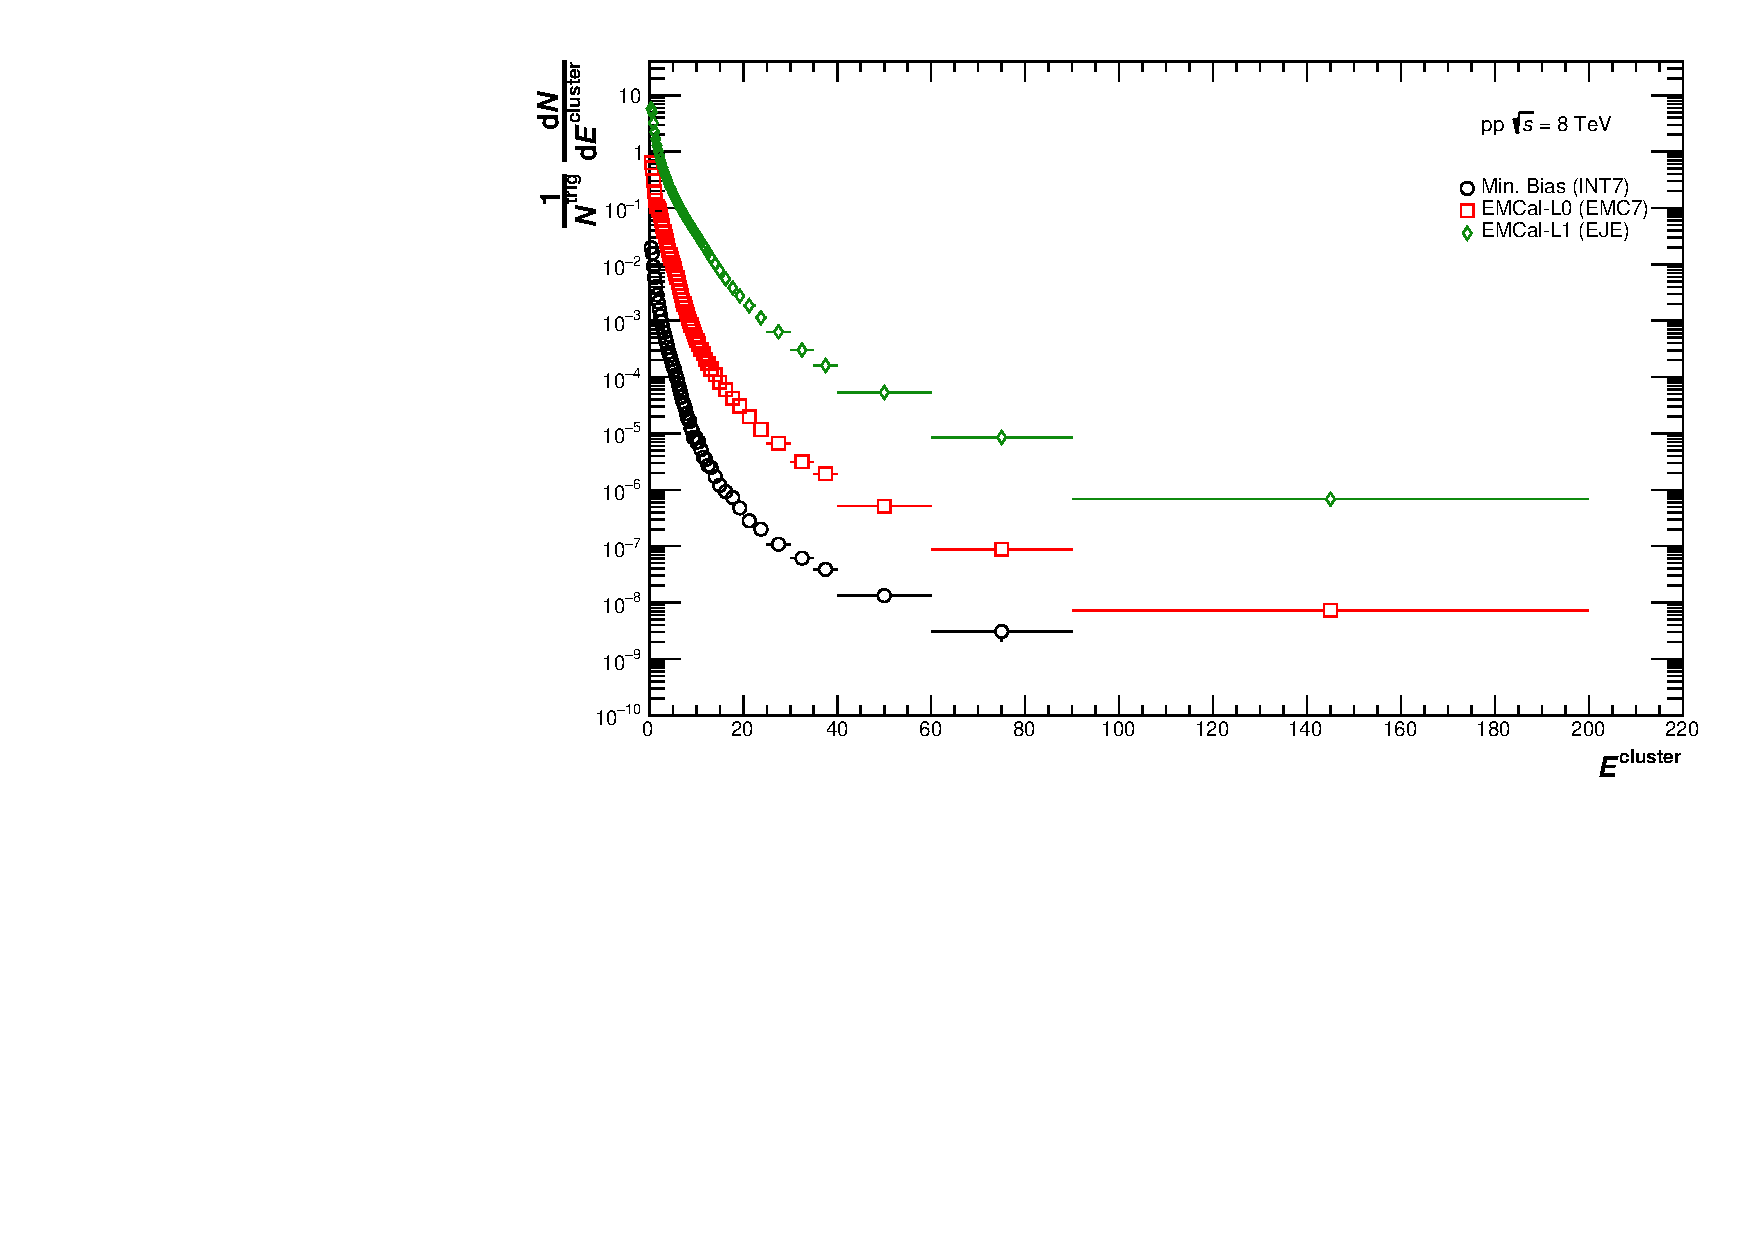
\includegraphics[width=15cm]{figures/TriggerClusters/clusters_R02.pdf}
    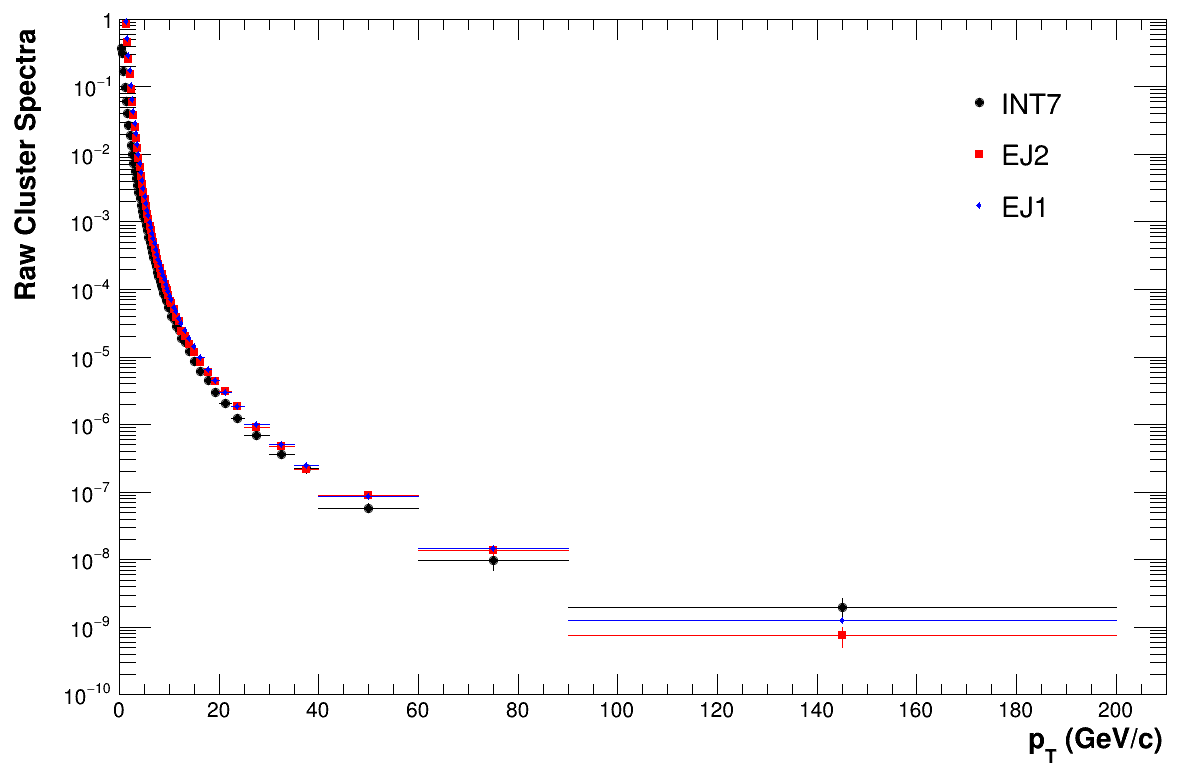
\includegraphics[width=15cm]{figures/pPbFigures/TriggerClusters/rawclusterspectra_alltriggers_R02.png}
    \caption{Trigger cluster yields for the INT7, EMC7, and EJE triggers in \pp (left), and for INT7, EJ2, and EJ1 triggers in \pPb (right). Scaling is required in order for the spectra to overlap.}
    \label{fig:triggerClusters}
\end{figure}

In the 2012 dataset, the downscale factors for the INT7 and EMC7 triggers were not recorded. For this reason, the triggered data must be corrected by the use of rejection factors. These trigger rejection factors are calculated by taking the ratio of the cluster yield between triggers with neighboring thresholds after correction for the trigger efficiency. In this case, the ratio of the EMC7 to INT7 triggers and the ratio of the EJE to EMC7 triggers are taken. A correction must be made for the trigger efficiency. This is done by taking the ratio of the EMCal trigger to minimum bias cluster yields in Monte Carlo. The ratio of cluster yields for different triggers without correction for the cluster trigger efficiency is shown in figure \ref{fig:RejectionFactorsUnscaled}. The plateaus are fit with an error function, and the flat region of the function is taken as the constant rejection factor. The ratios of the cluster yields for different triggers in data after the trigger efficiency correction are shown in Figure~\ref{fig:RejectionFactors}. The low-\pT region shows the range in which the trigger has not yet reached maximum efficiency and the behavior of the cluster spectra is not described by the Monte Carlo. The measurement is reliable at momenta in the region where the ratios reach a plateau. These plateaus are fit with a constant to find the rejection factor and its associated uncertainty. The jet spectrum for the EMC7 trigger is then divided by the rejection factor derived from the EMC7 to INT7 trigger cluster ratio, while the jet spectrum for the EJE trigger is divided by both rejection factors.

\begin{figure}
    \centering
    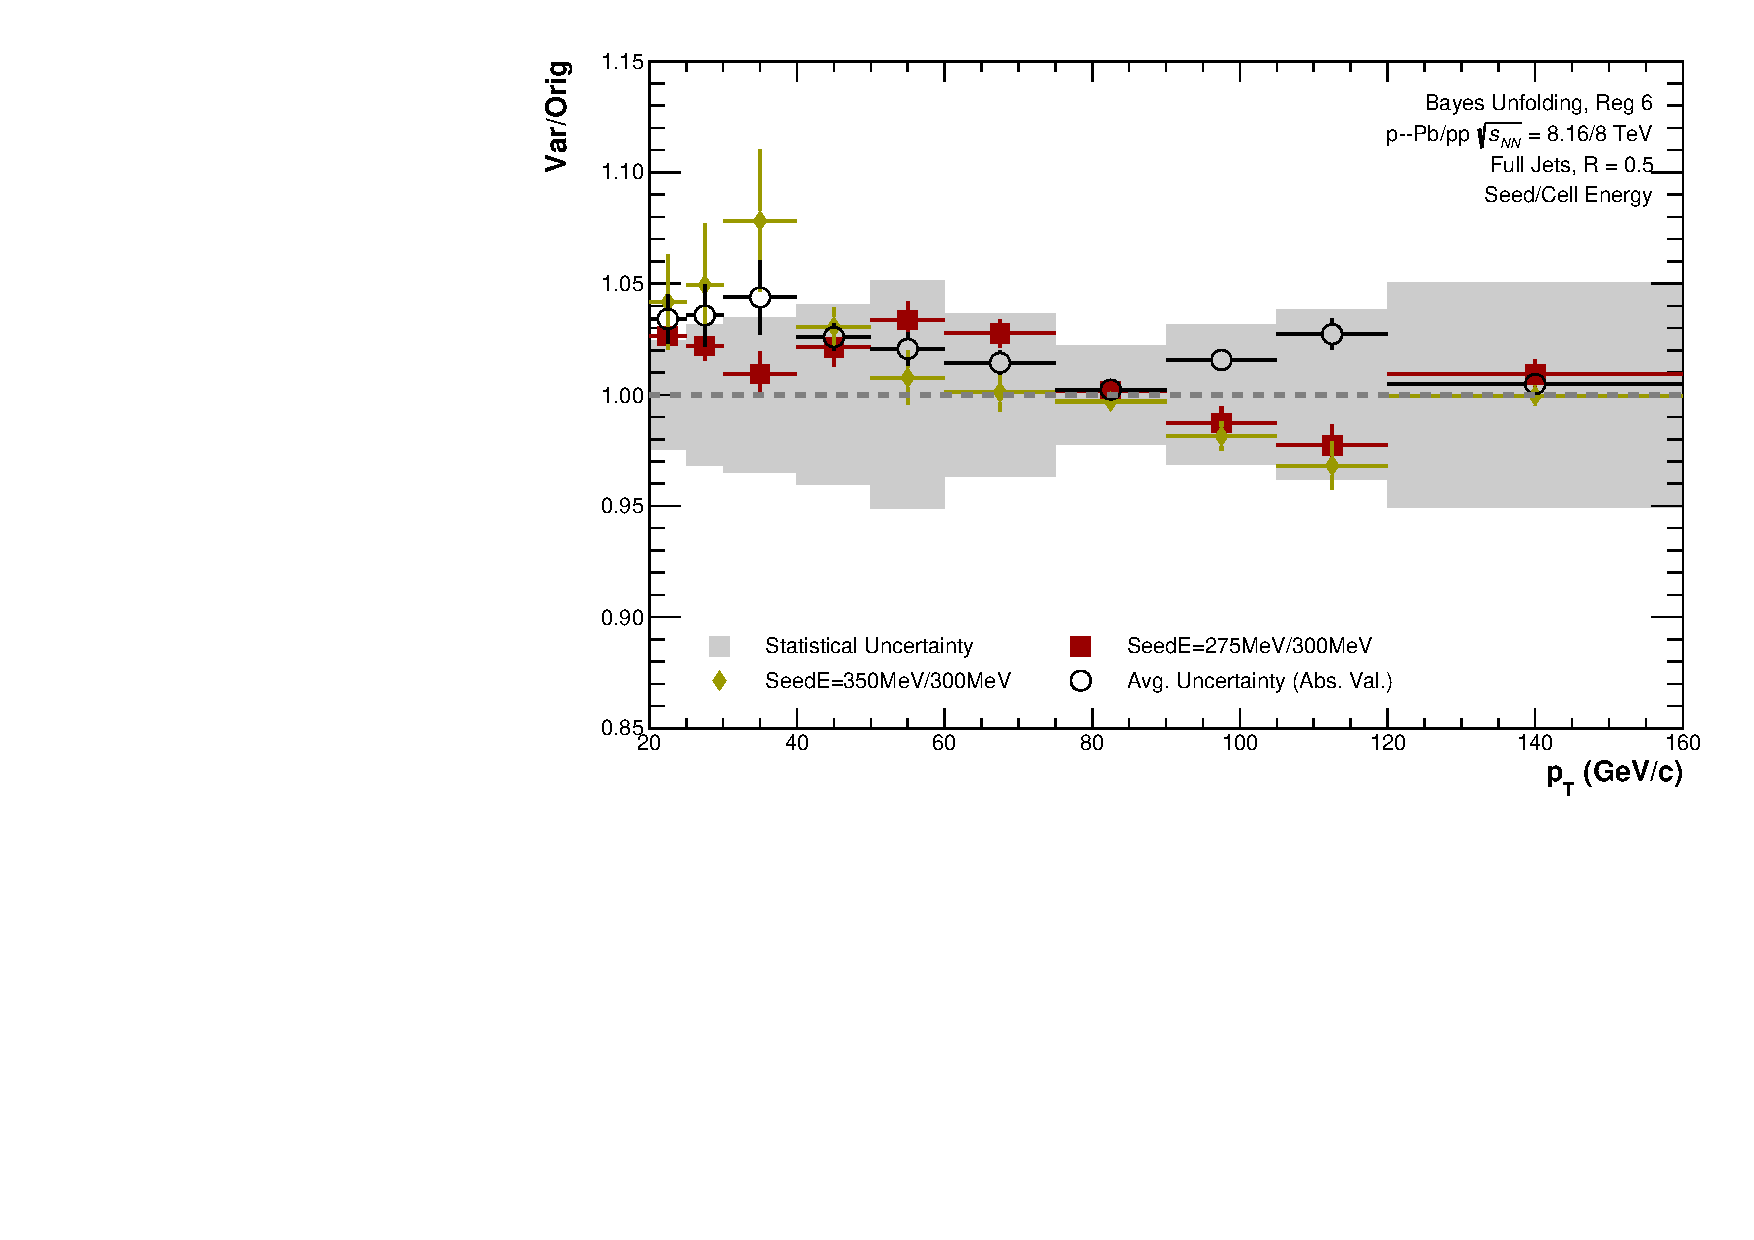
\includegraphics[width=15cm]{figures/RejectionFactors/RF_R02_Unscaled_Default.pdf}
    \caption{Rejection factors for the EMC7 trigger and the EJE trigger, found by taking the ratio of the event-normalized trigger yields of the EMC7/INT7 triggers and EJE/EMC7 triggers, respectively.}
    \label{fig:RejectionFactorsUnscaled}
\end{figure}


\begin{figure}[hbt!]
    \centering
    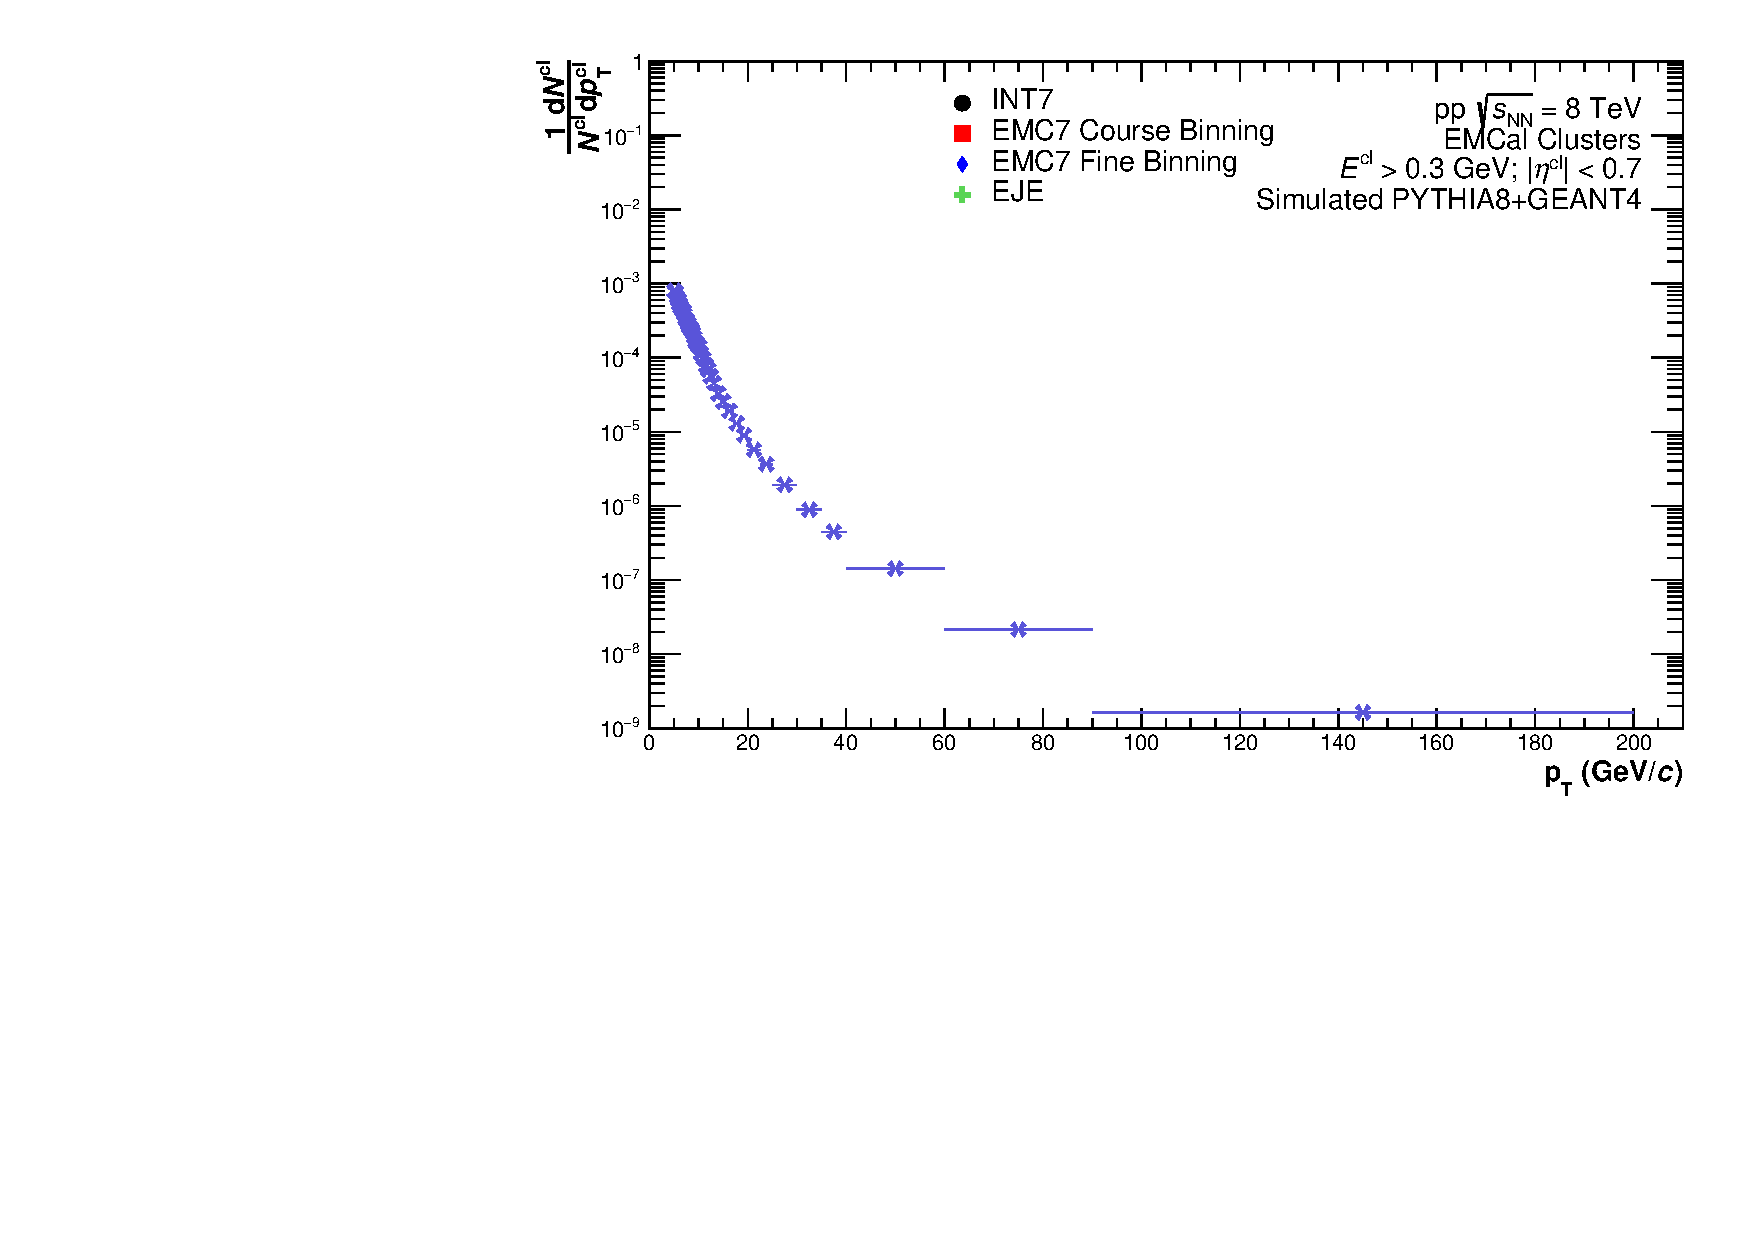
\includegraphics[width=15cm]{figures/RejectionFactors/RF_R02_Default.pdf}
    \caption{Rejection factors in \pp collisions for the EMC7 trigger and the EJE trigger. The ratio is taken of the event-normalized trigger yields of the EMC7/INT7 triggers and EJE/EMC7 triggers and scaled by the cluster trigger efficiency. The plateau is fit with a constant to find the rejection factor.}
    \label{fig:RejectionFactors}
\end{figure}

In the \pPb dataset, the observed integrated luminosity can be used to scale the spectra in place of the rejection factors. The detector readout speed is determined by the slowest detector in the trigger cluster. If that detector is removed from the cluster, more collisions can be recorded. If more than one trigger cluster is used in the analysis, the effective live time can be different. As there is typically at least one trigger shared by two clusters, this shared trigger can be used to compare the clusters and find the required scale corrections. Because the corrections factorize, the integrated luminosity of the trigger can be calculated based on the event count and the downscaling of the minimum bias trigger. In the \pp dataset, no overlap existed between the clusters, so the rejection factors were used instead.


\begin{figure}[hbt!]
    \centering
    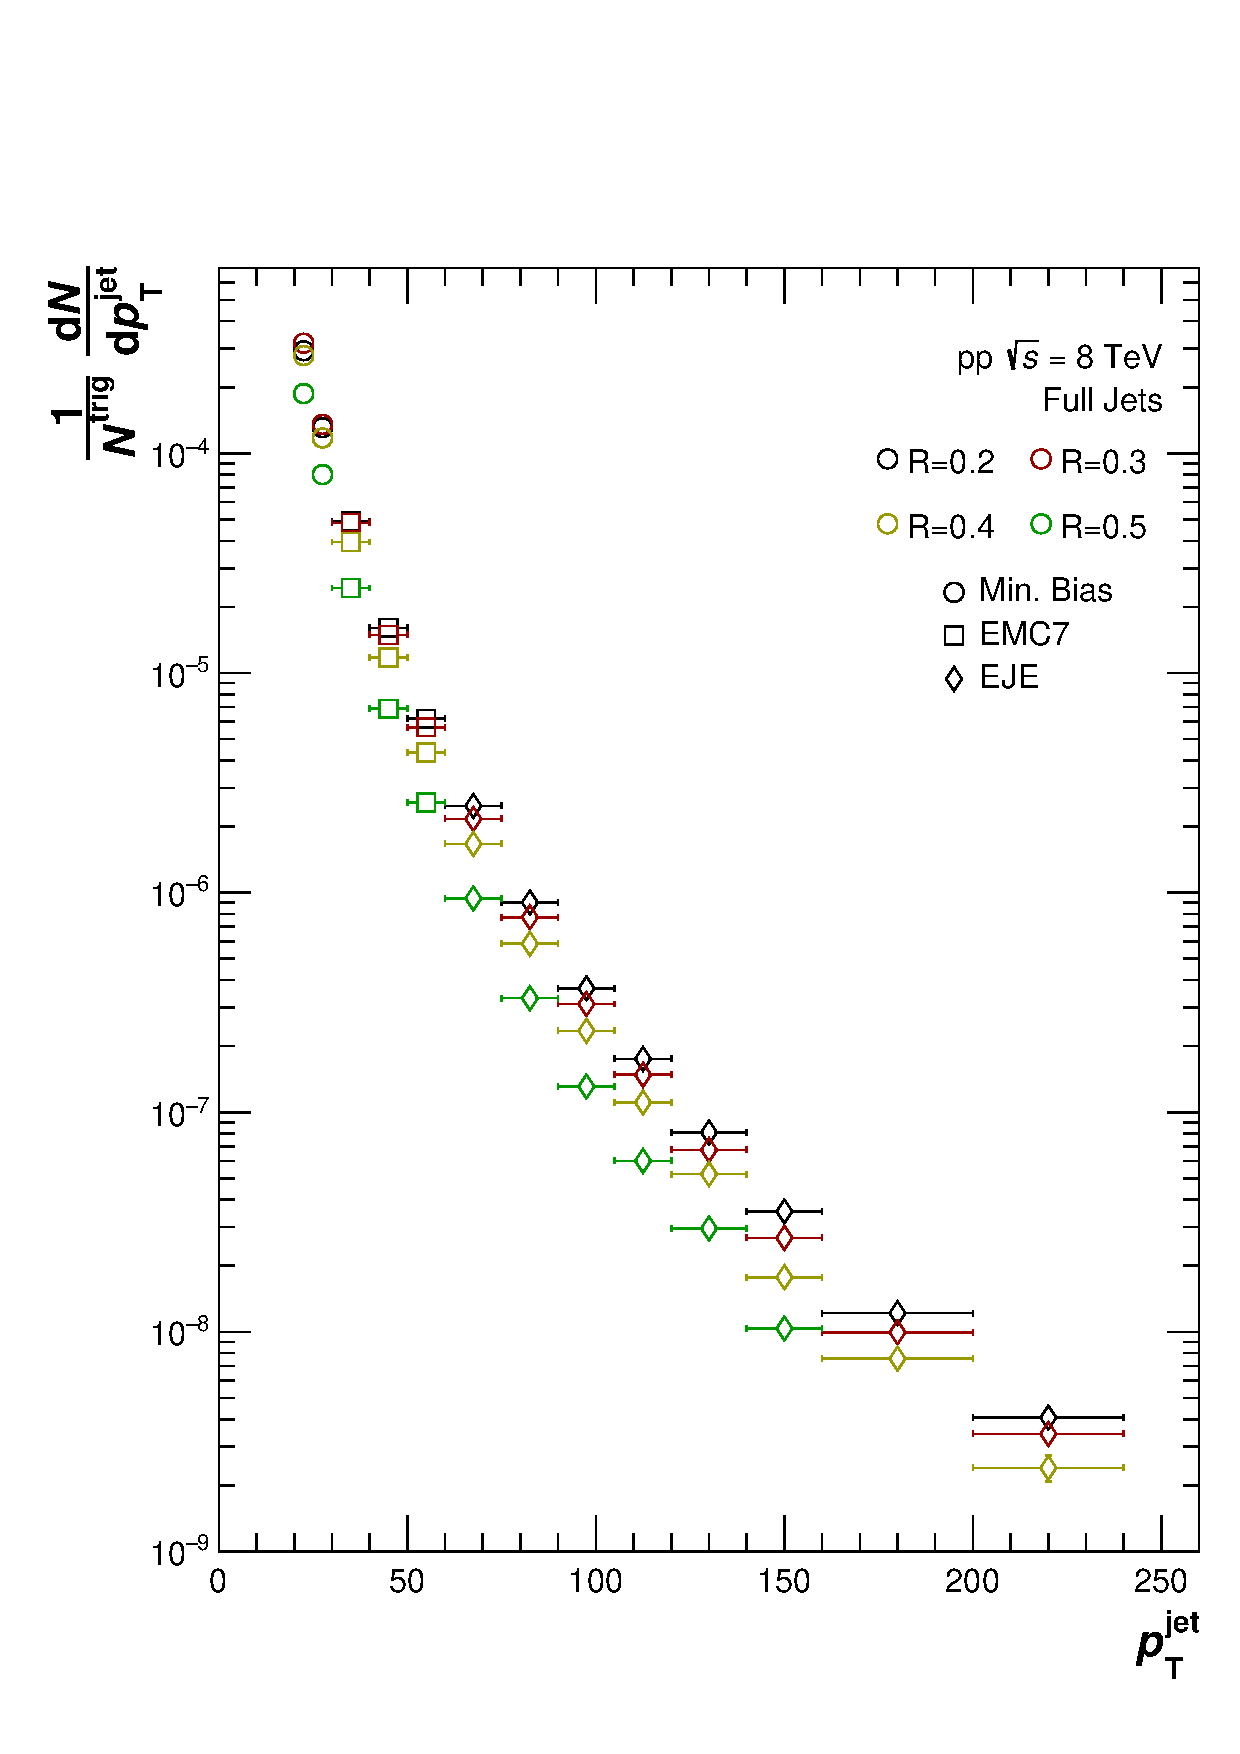
\includegraphics[width=0.49\textwidth]{figures/CorrRawSpec/corrRawSpec.pdf}
    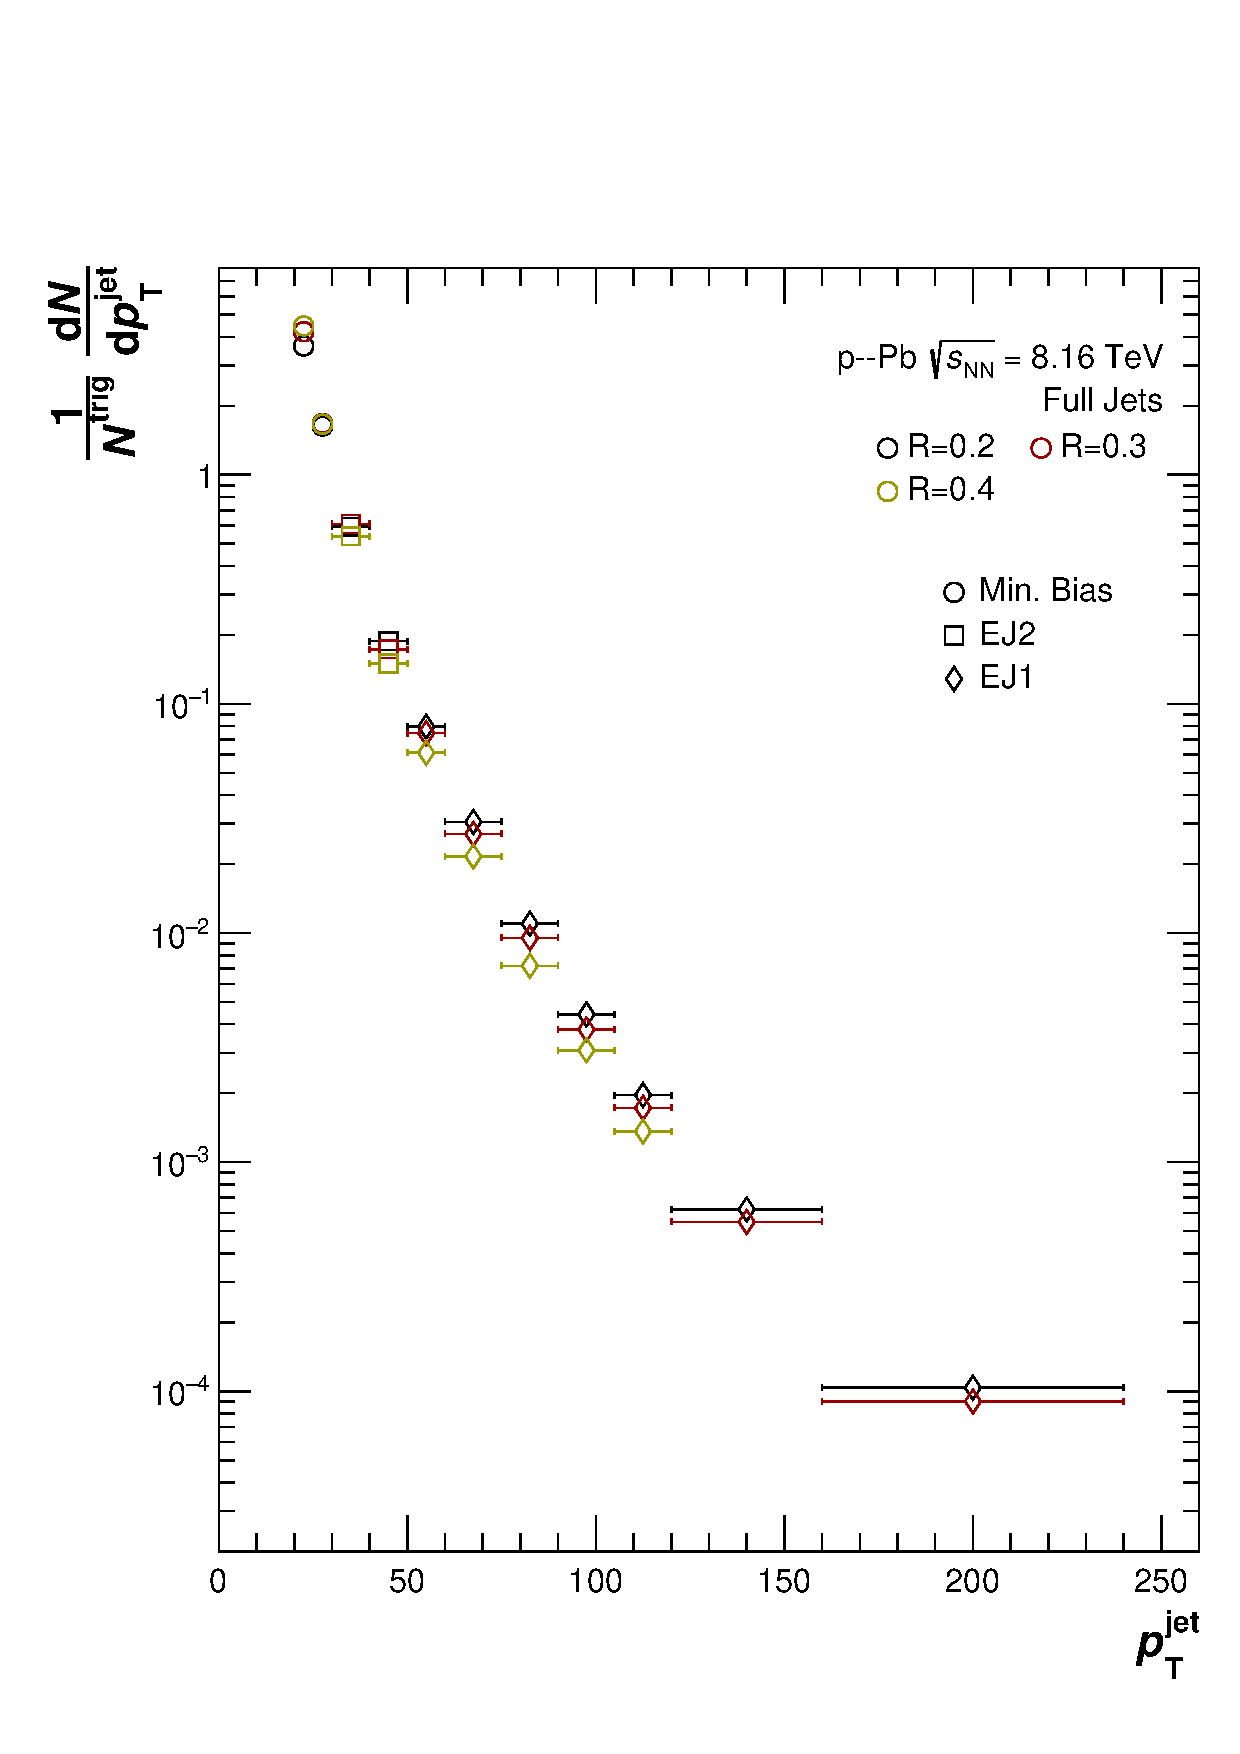
\includegraphics[width=0.49\textwidth]{figures/pPbFigures/CorrRawSpec/corrRawSpec.pdf}
    \caption{Jet spectra in \pp (left) and \pPb (right) collisions for the three triggers after corrections for various jet radii.}
    \label{fig:CorrRawSpec}
\end{figure}

The full spectrum before unfolding is constructed by combining the spectra from the three trigger classes after the application of the scaling factors. Figure~\ref{fig:CorrRawSpec} shows the comparison of the spectra from the three triggers in \pp for jets with different jet radii. 

\subsection{Scaling of the Jet Spectrum}
\label{sec:xsecNomalization}

Since the jet yield was measured only in the EMCal acceptance, a correction for the limited acceptance has to be applied. The acceptance correction is

\begin{equation}
    A = \frac{\Delta\eta \Delta\phi}{2\pi}
\end{equation}

where $\Delta\eta = 1.4 - 2R$ and $\Delta\phi = 1.745 - 2R$ for \pp, and $\Delta\eta = 1.4 - 2R$ and $\Delta\phi = 1.887 - 2R$ for
\pPb. The azimuthal correction is different for the \pPb dataset because extra EMCal modules were added during long shutdown 1, between run 1 and run 2.

The number of events has to be corrected for the vertex finding efficiency. This is done by dividing the spectrum by the efficiency, which is defined as the fraction of events before and after vertex selection and is evaluated before the vertex-z cut. The vertex finding efficiency has been determined from the event counters for accepted and rejected events to be 94.8$\%$ for INT7, 99.2$\%$ for EMC7, and 99.6$\%$ for EJE. EMCal triggered events have a higher multiplicity on average, so more tracks contribute to the vertex reconstruction, especially in pp-collisions. Since luminosity scaling is used in the \pPb dataset instead of the rejection factors, the vertex finding efficiency from the INT7 reference trigger is used for all triggers. In this case, the INT7 vertex finding efficiency is 98.6\%.

\subsection{Background subtraction}
\label{sec:backgroundSubtraction}

In hadronic collisions, reconstructed jets from hard scatterings are not the only particles in the event. Contributions from softer processes will sometimes get clustered together and reconstructed as a jet. Other than in high-multiplicity events, this contribution in \pp collisions is small, but in \pPb collisions, it is large enough that it must be corrected for.

The method used in this analysis to subtract the underlying event was developed by the CMS collaboration for sparse background environments and is termed the $\rho$-sparse method~\cite{CMS:2012rmf}. This method defines the transverse momentum background density as 

\begin{equation}
    \rho_{\text{CMS}} = median\{\frac{{\text{\pT}}_{jet}^{k_T}}{A_{jet}^{k_T}}\} \cdot C
\end{equation}

\noindent
where ${\text{\pT}}_{jet}^{k_T}$ is the transverse momentum of a jet clustered with the $k$\textsubscript{T} algorithm, $A_{jet}^{k_T}$ is the area of that jet, and $C$ is the particle occupancy factor, used to account for regions without any particles. It is defined as

\begin{equation}
    C = \frac{\Sigma_{\text{j}}A_{\text{j}}}{A_{\text{acc}}}
\end{equation}

\noindent
where $A_\text{j}$ is the area of each $k$\textsubscript{T} jet with at least one real track and $A_{\text{acc}}$ is the total particle acceptance. It can be thought of as the covered area divided by the total area, showing how full or empty the event is. The $\rho$ distribution for all three triggers is shown in Figure~\ref{fig:Rho_distribution} for jets with resolution parameter $R$ = 0.2, 0.3, and 0.4. The effect from background is greatest at low momenta and the effect decreases with increasing jet \pT. Since the INT7 trigger covers the low momentum range for this measurement, only the $\rho$ distribution for the INT7 trigger is used for this analysis. For $R$ = 0.2, the distribution is smoothly falling with a maximum at zero. With increasing jet resolution parameter, the distribution becomes more peaked at zero and has a longer tail at high $\rho$ values. This is due to the fact that the highest momentum (signal) jet is excluded from the background calculation, and larger radius jets become increasing difficult to fit inside the acceptance without overlapping with the highest momentum jet. For this reason, and because the background distribution is calculated per unit area, the calculation of $\rho$ at a $k$\textsubscript{T} jet resolution parameter of $R$ = 0.2 is used for all jet radii.

A possible alternative to this method bypasses the limitation of the EMCal acceptance~\cite{anaNoteMConnors}. Instead of calculating the background from a cone within the EMCal acceptance, the entire TPC acceptance is used to calculate the background. A scaling factor is then applied to $\rho$, defined as 

\begin{equation}
    S = \frac{E_{\text{EMC}}+\text{\pT}_\text{EMC}}{\text{\pT}_\text{TPC}}\frac{A_{\text{TPC}}}{A_{\text{EMC}}}
\end{equation}

\noindent
The first term is the ratio of the sum of the total energy from clusters in the EMCal after the hadronic correction is applied and the total momentum of all charged track pointing towards the EMCal acceptance to the total momentum of all charged tracks within the TPC acceptance. The second term is a normalization factor for the relative acceptances of the TPC and EMCal. As an extension of this thesis, this background subtraction technique will be applied to the \pPb data in order to compare these methods.


\begin{figure}[hbt!]
  \centering
  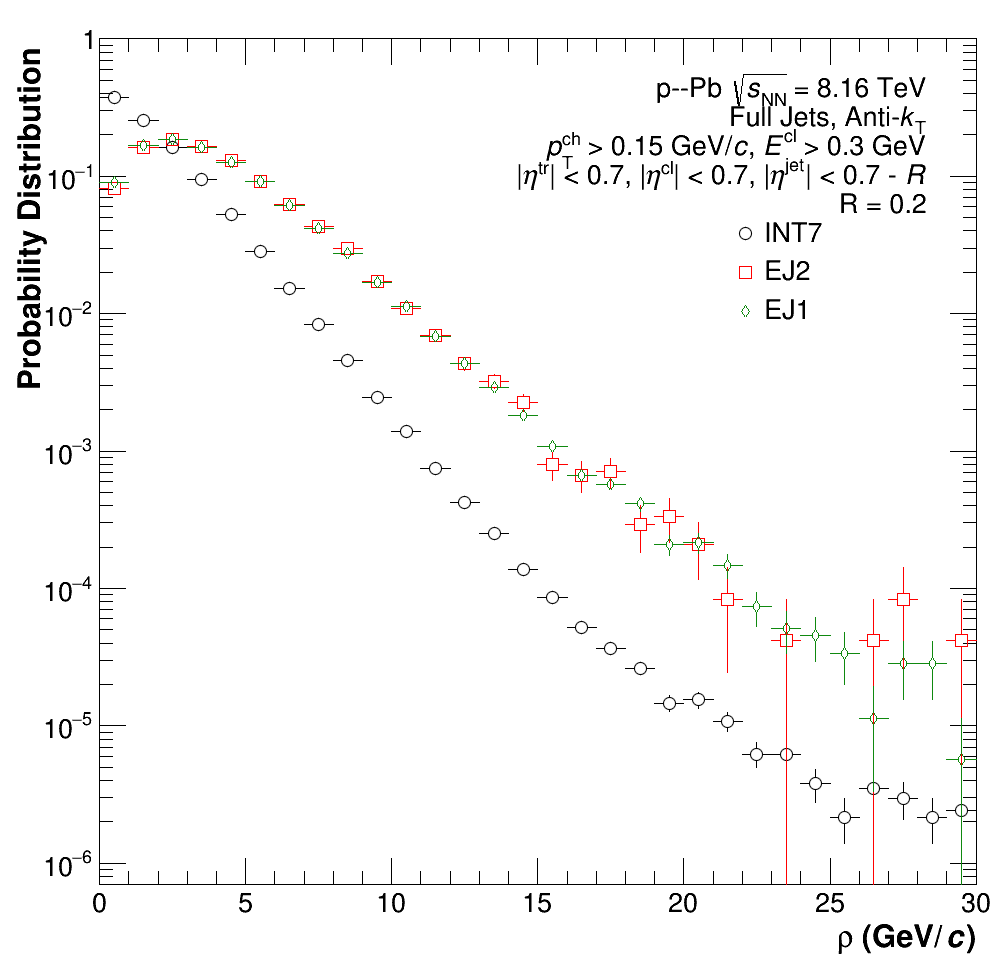
\includegraphics[width=0.49\textwidth]{figures/pPbFigures/BGSubtraction/plotRho_R02.png}
  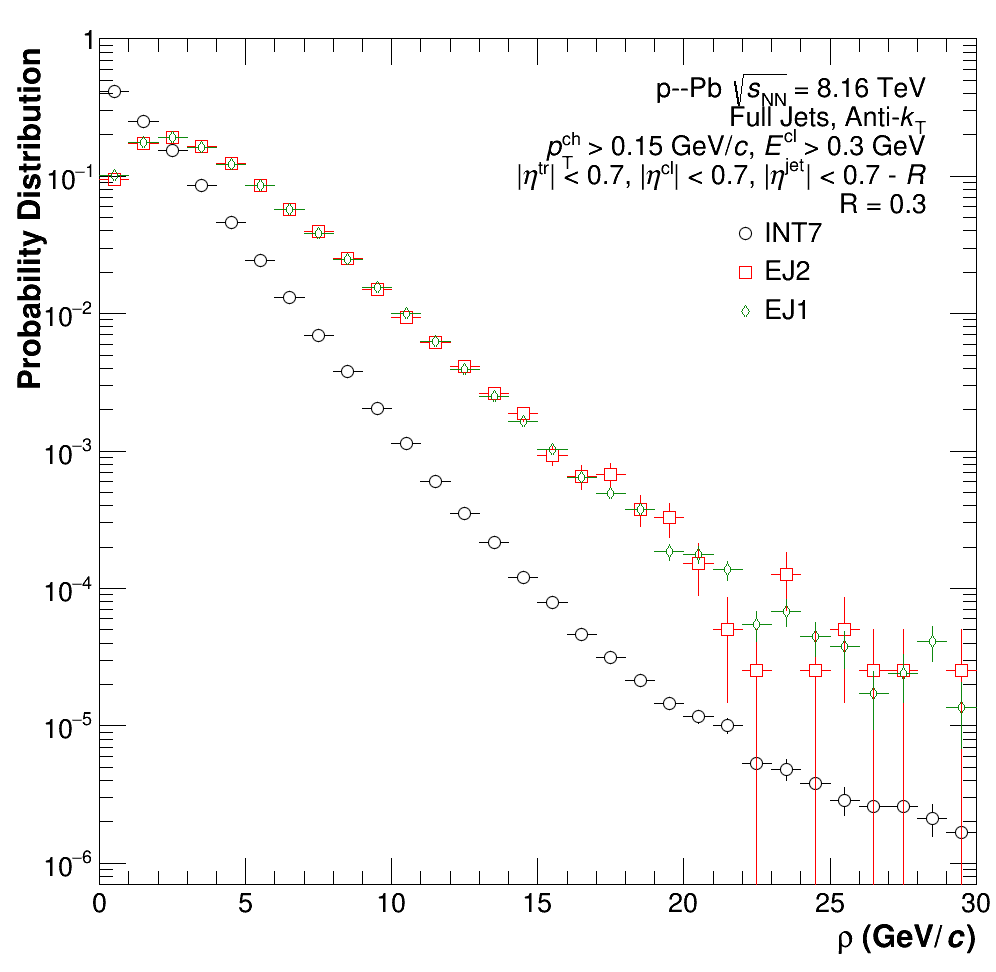
\includegraphics[width=0.49\textwidth]{figures/pPbFigures/BGSubtraction/plotRho_R03.png}
  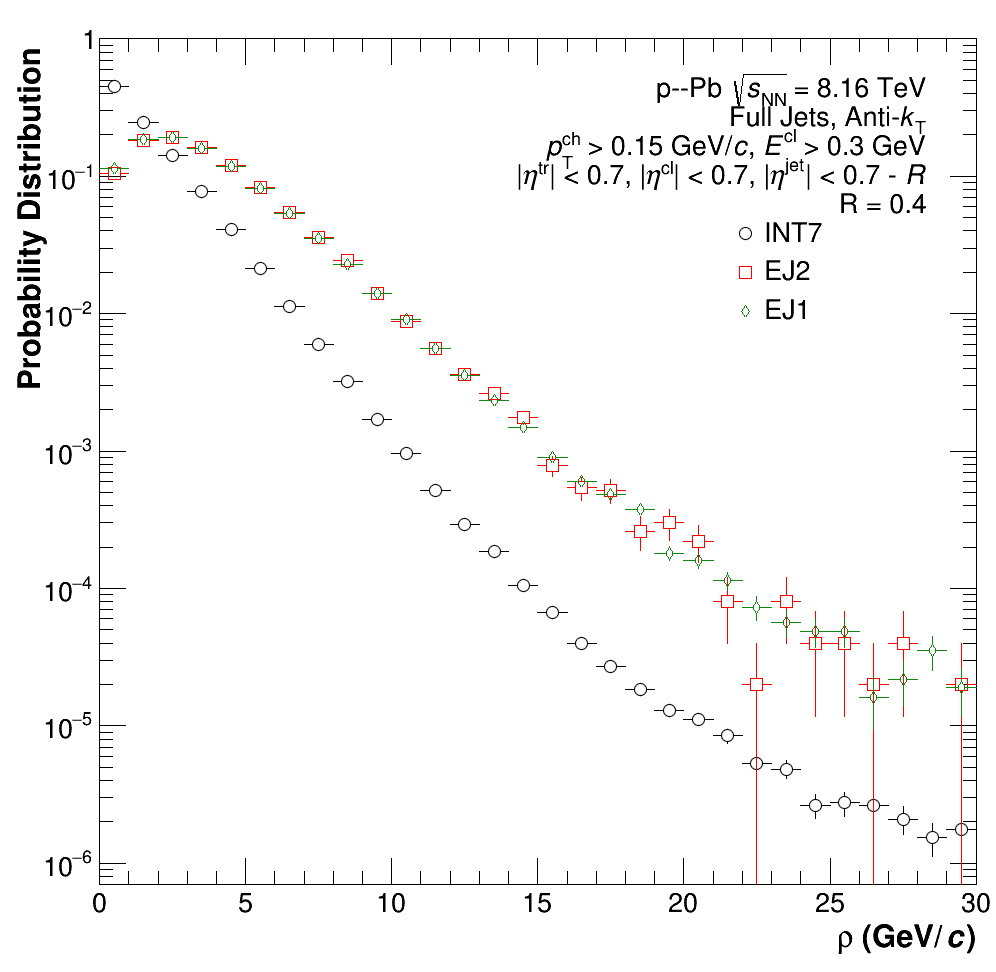
\includegraphics[width=0.49\textwidth]{figures/pPbFigures/BGSubtraction/plotRho_R04.png}
  \caption{Rho distribution for the INT7, EJ2, and EJ1 triggers in \pPb collisions for jets with resolution parameter $R$ = 0.2, 0.3, and 0.4.}
  \label{fig:Rho_distribution}
\end{figure}

The corrected jet momentum is then calculated as 

\begin{equation}
    \text{\pT}_{,jet}^{\text{corr}} = \text{\pT}_{,jet}^{\text{raw}} - \rho_{\text{CMS}} \cdot A_{\text{jet}}.
\end{equation}

\noindent
The background is calculated on an event-by-event basis using only particles within the jet acceptance and assumes a uniform background density. The true background density for each jet fluctuates around this average background density. This effect of background fluctuations is accounted for during the unfolding procedure by first using the random cones approach~\cite{ALICE:2012nbx} to find the $\delta$-\pT distribution. A cone with resolution parameter equivalent to the jet resolution parameter is randomly placed inside the $\eta-\phi$ acceptance of each event. The cone cannot overlap with the highest momentum jet and must be contained within the jet acceptance. The background fluctuations are then defined as 

\begin{equation}
    \delta \text{\pT} = \text{\pT}_\text{,RC} - \rho_{\text{CMS}} \pi R_{\text{cone}}^2
\end{equation}

\noindent
where $\text{\pT}_\text{,RC}$ is the \pT of the random cone and $R_{\text{cone}}$ is its resolution parameter. The $\delta$-\pT distribution for all three triggers is shown in Figure~\ref{fig:DeltaPt_distribution} for jets with resolution parameter $R$ = 0.2, 0.3, and 0.4. The distribution for INT7 is used since this is where the background dominates. The distribution is centered at zero with a steep tail toward negative values caused by fluctuations from soft processes. The longer tail toward positive values originates from both background fluctuations and signal.


\begin{figure}[hbt!]
  \centering
  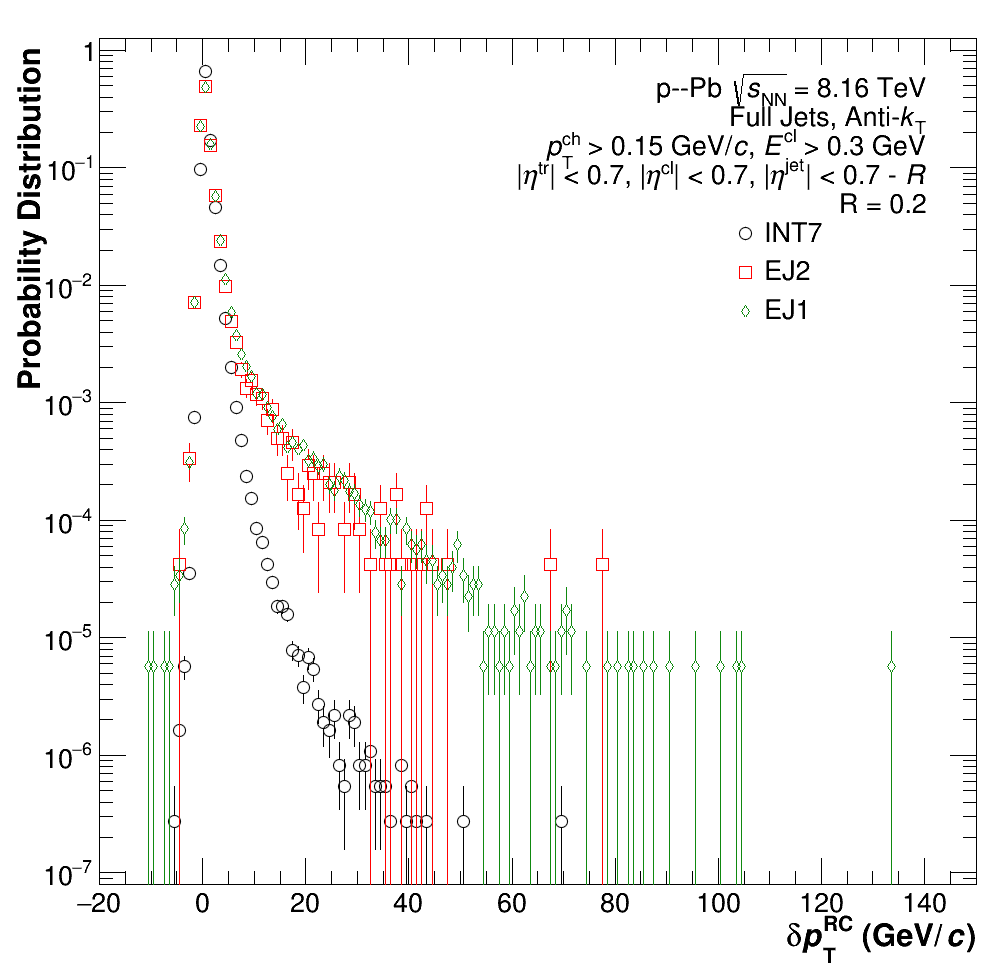
\includegraphics[width=0.49\textwidth]{figures/pPbFigures/BGSubtraction/plotDpT_R02.png}
  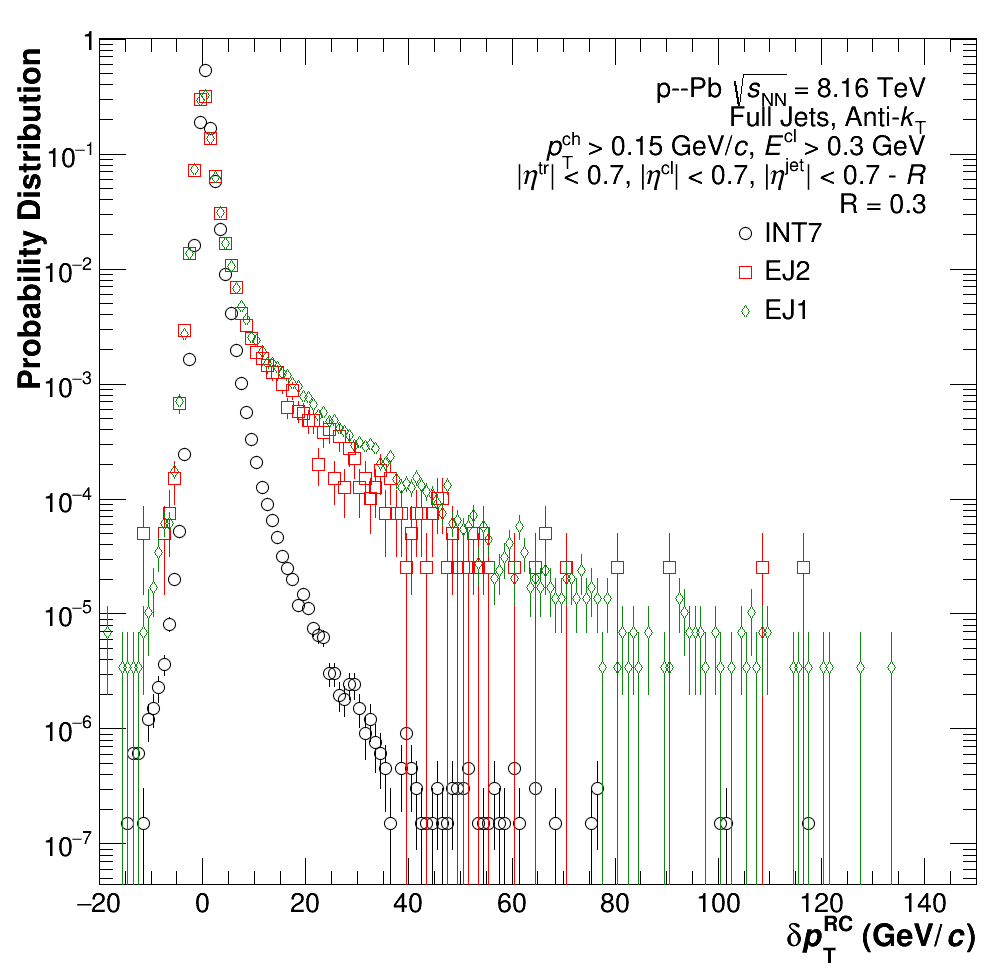
\includegraphics[width=0.49\textwidth]{figures/pPbFigures/BGSubtraction/plotDpT_R03.png}
  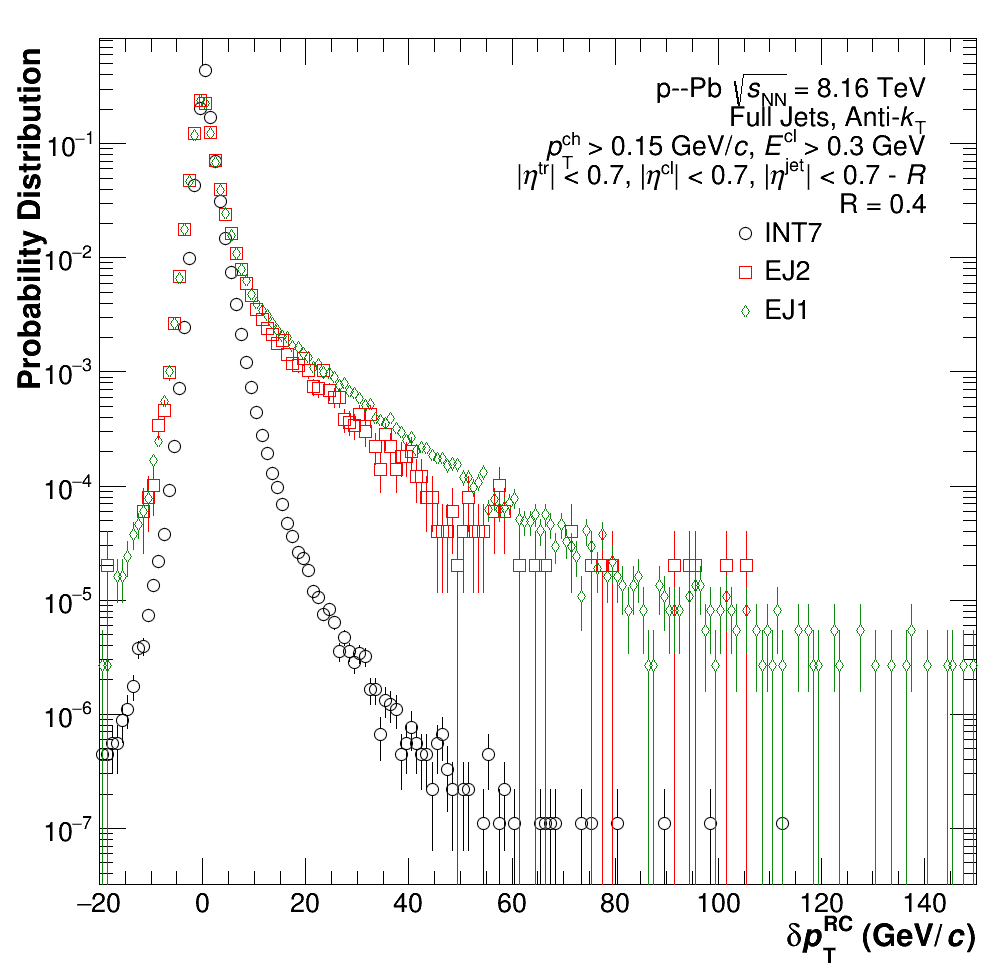
\includegraphics[width=0.49\textwidth]{figures/pPbFigures/BGSubtraction/plotDpT_R04.png}
  \caption{$\delta$-\pT distribution for the INT7, EJ2, and EJ1 triggers in \pPb collisions for jets with resolution parameter $R$ = 0.2, 0.3, and 0.4.}
  \label{fig:DeltaPt_distribution}
\end{figure}

\subsection{Instrumental Response}
\label{sec:InstResponse}


\begin{figure}[hbt!]
    \centering
    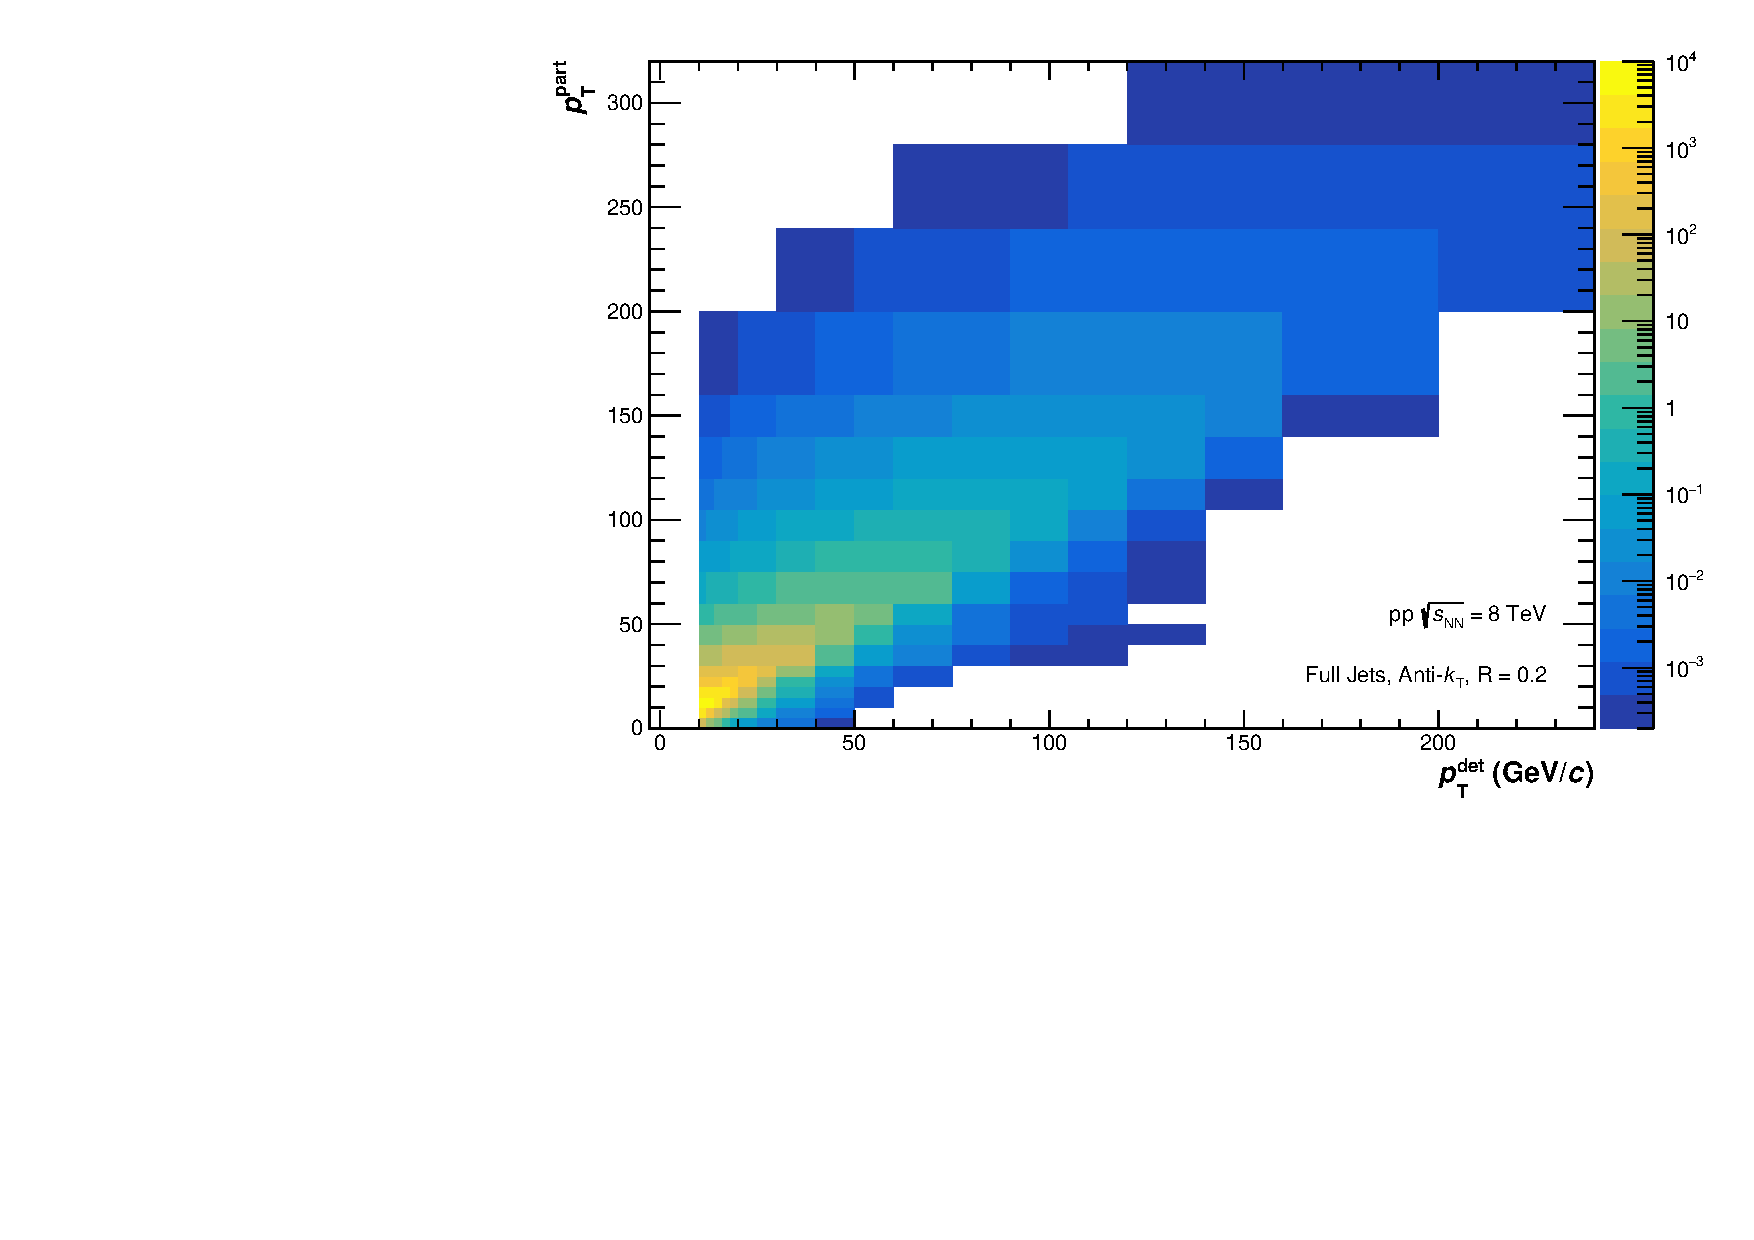
\includegraphics[width=0.95\textwidth]{figures/Response/Response_R02.pdf}
    \caption{Response matrix for \pp collisions for jets with resolution parameter $R$ = 0.2.}
    \label{fig:ResponseMatrix}
\end{figure}

PYTHIA8 events were fully propagated through a simulation of the ALICE detector using GEANT3~\cite{Brun:1987ma} to form a detector response matrix. GEANT is a software package used to simulate particle interactions with detector materials. This response matrix compares jets at generator level (i.e. PYTHIA), typically referred to as "particle level" or "truth level" jets, to jets after propagation through GEANT and reconstruction, typically referred to as "detector level" or "reconstructed level" jets. Detector or reconstructed level is also used to describe data that have not yet been corrected with the response matrix, while particle or truth level is also used to describe data that have been corrected by the response matrix. The response matrix is shown in Figure~\ref{fig:ResponseMatrix} for \pp collisions, which is used to correct the measured jet distributions during unfolding. PYTHIA8 is referred to as the "prior," because by using these simulated events to form the response matrix, an assumption is made that the true jet spectrum looks similar to the jet spectrum produced by PYTHIA8. In order to account for background fluctuations in \pPb events, the response matrix from simulated \pp events at 8.16 TeV was smeared by the $\delta$-\pT distribution from random cones. The residual distribution can be derived in order to characterize the response matrix, which is defined as

\begin{equation}
    \frac{p_\mathrm{T,jet}^{\text{det}} - p_\mathrm{T,jet}^{\text{part}}}{p_\mathrm{T,jet}^{\text{part}}}
\end{equation}

\noindent
where "det" indicates the detector/reconstructed level and "part" indicates the particle/truth level. The residual distribution is used to form the jet energy scale and the jet energy resolution, seen in Figure~\ref{fig:EnergyScale} for \pp and Figure~\ref{fig:EnergyScalepPb} for \pPb. The left plot shows the jet energy scale shift, quantified as the mean of the residual distribution as a function of the true jet \pT. If all jets at particle level were properly reconstructed at detector level, the jet energy scale would be zero. We see a mild $R$ dependence, indicating that jets with a smaller resolution parameter are reconstructed correctly less often than large-$R$ jets. A relative negative shift of around 30\% at $p_\mathrm{T}^\mathrm{jet}$ = 100 GeV/$c$ is present due to finite tracking efficiency. At roughly 60 GeV/$c$, jets are reconstructed correctly more often than at any other \pT. Below this value, the energy scale falls steeply. Above this value, the energy scale decreases gradually toward higher \pT. The right plot shows the jet energy resolution which is quantified as the root mean squared of the distribution of residuals. We observe that the jet energy resolution is relatively flat for fully reconstructed jets at higher \pT due to the contribution from the EMCal. At low \pT, before the EMCal reaches maximum efficiency, the jet energy resolution rises quickly.


\begin{figure}[hbt!]
    \centering
    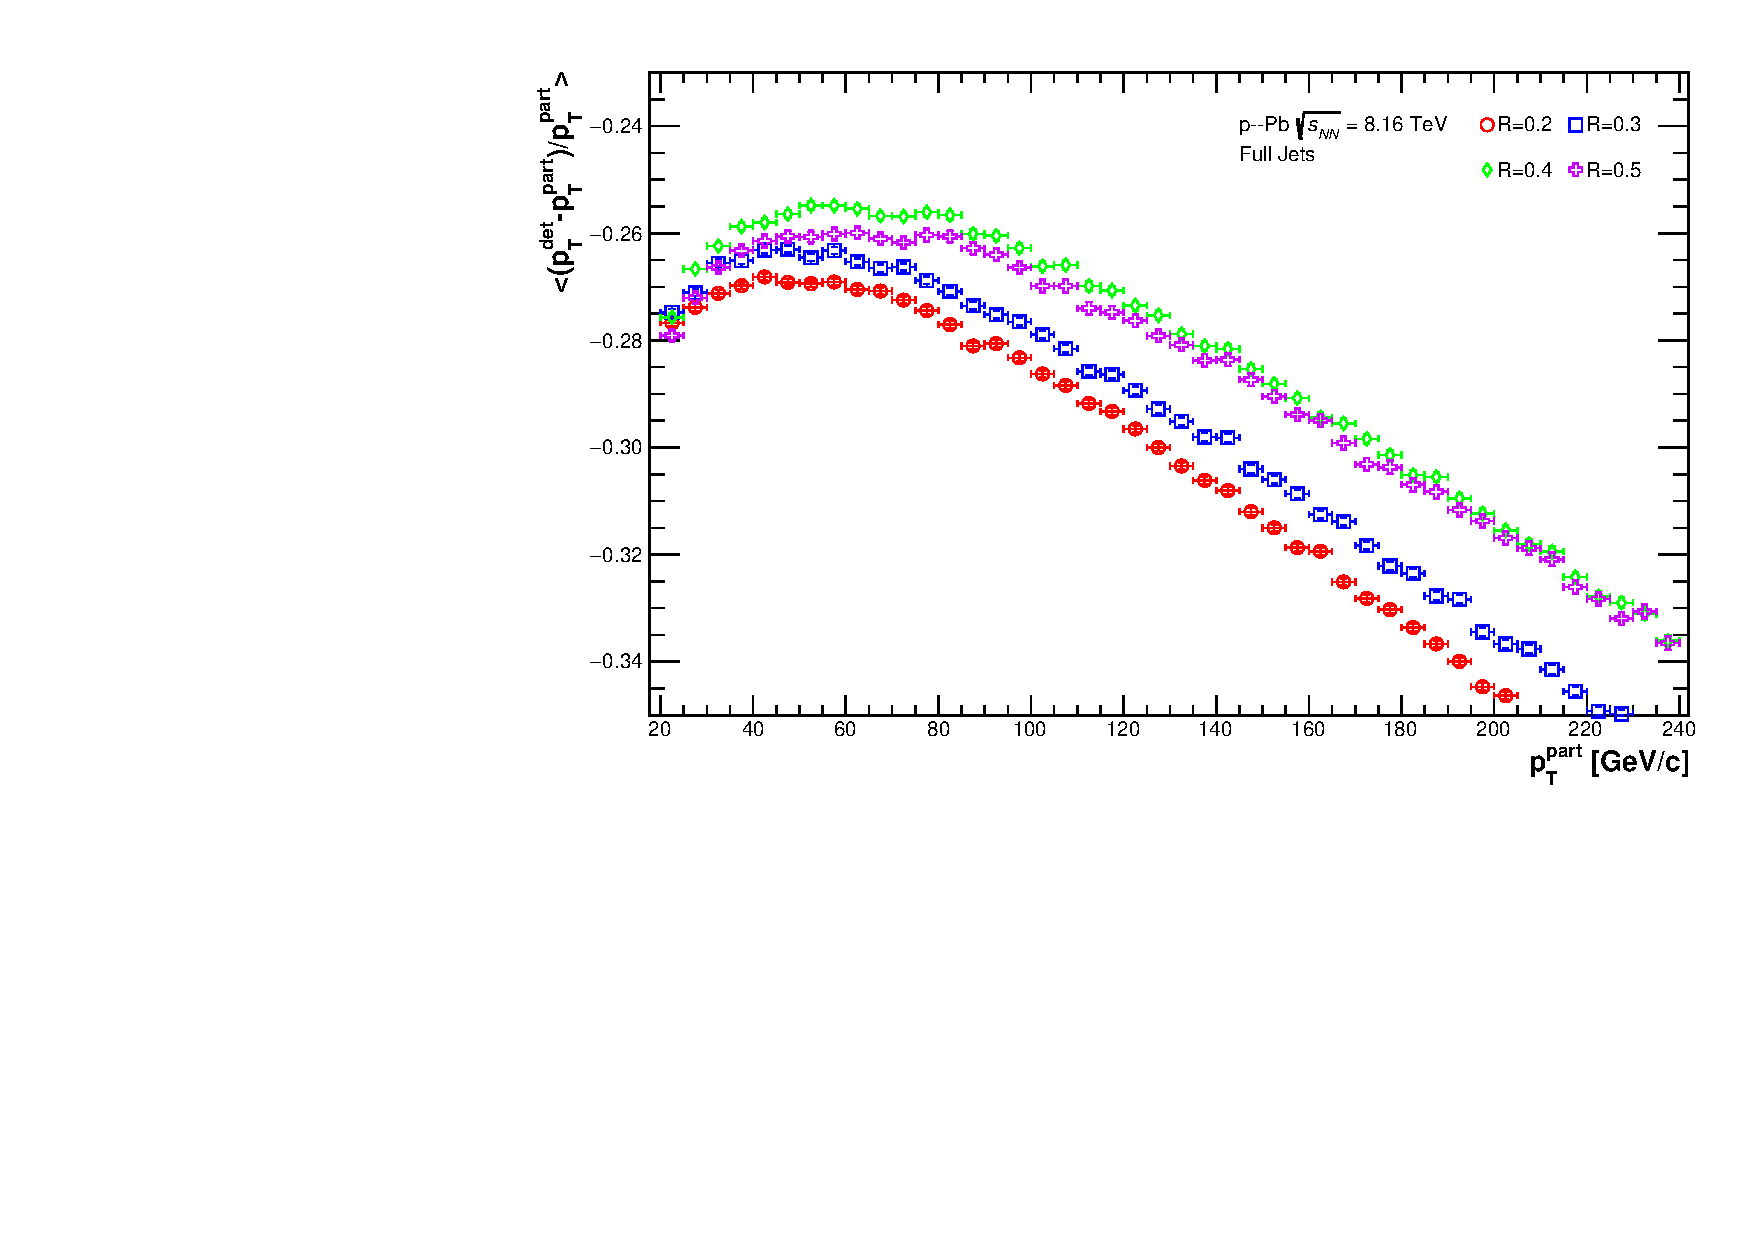
\includegraphics[width=0.49\textwidth]{figures/EnergyScale/EnergyScaleMean.pdf}
    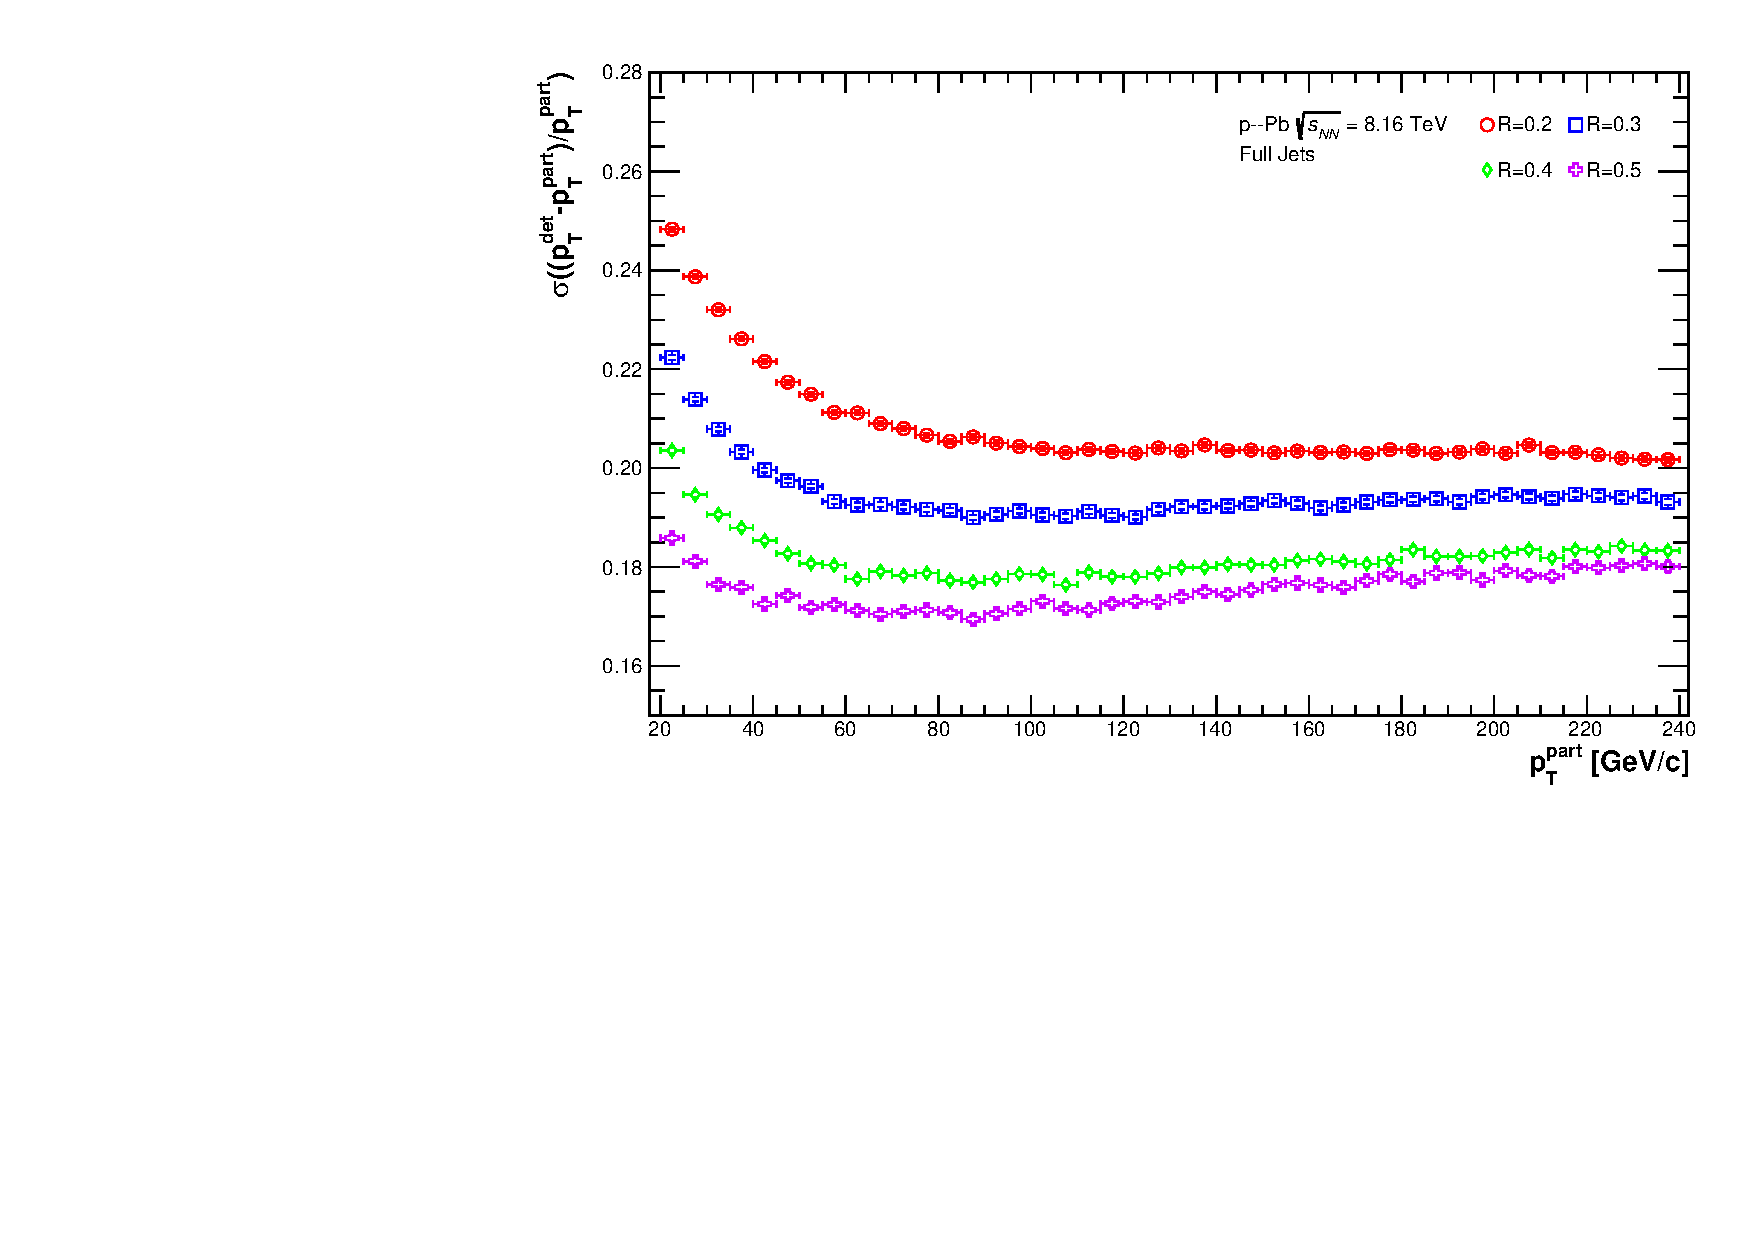
\includegraphics[width=0.49\textwidth]{figures/EnergyScale/EnergyScaleWidth.pdf}
    \caption{Jet energy scale (left) and jet energy resolution (right) showing the instrumental response to jets in \pp collisions.}
    \label{fig:EnergyScale}
\end{figure}

\begin{figure}[hbt!]
    \centering
    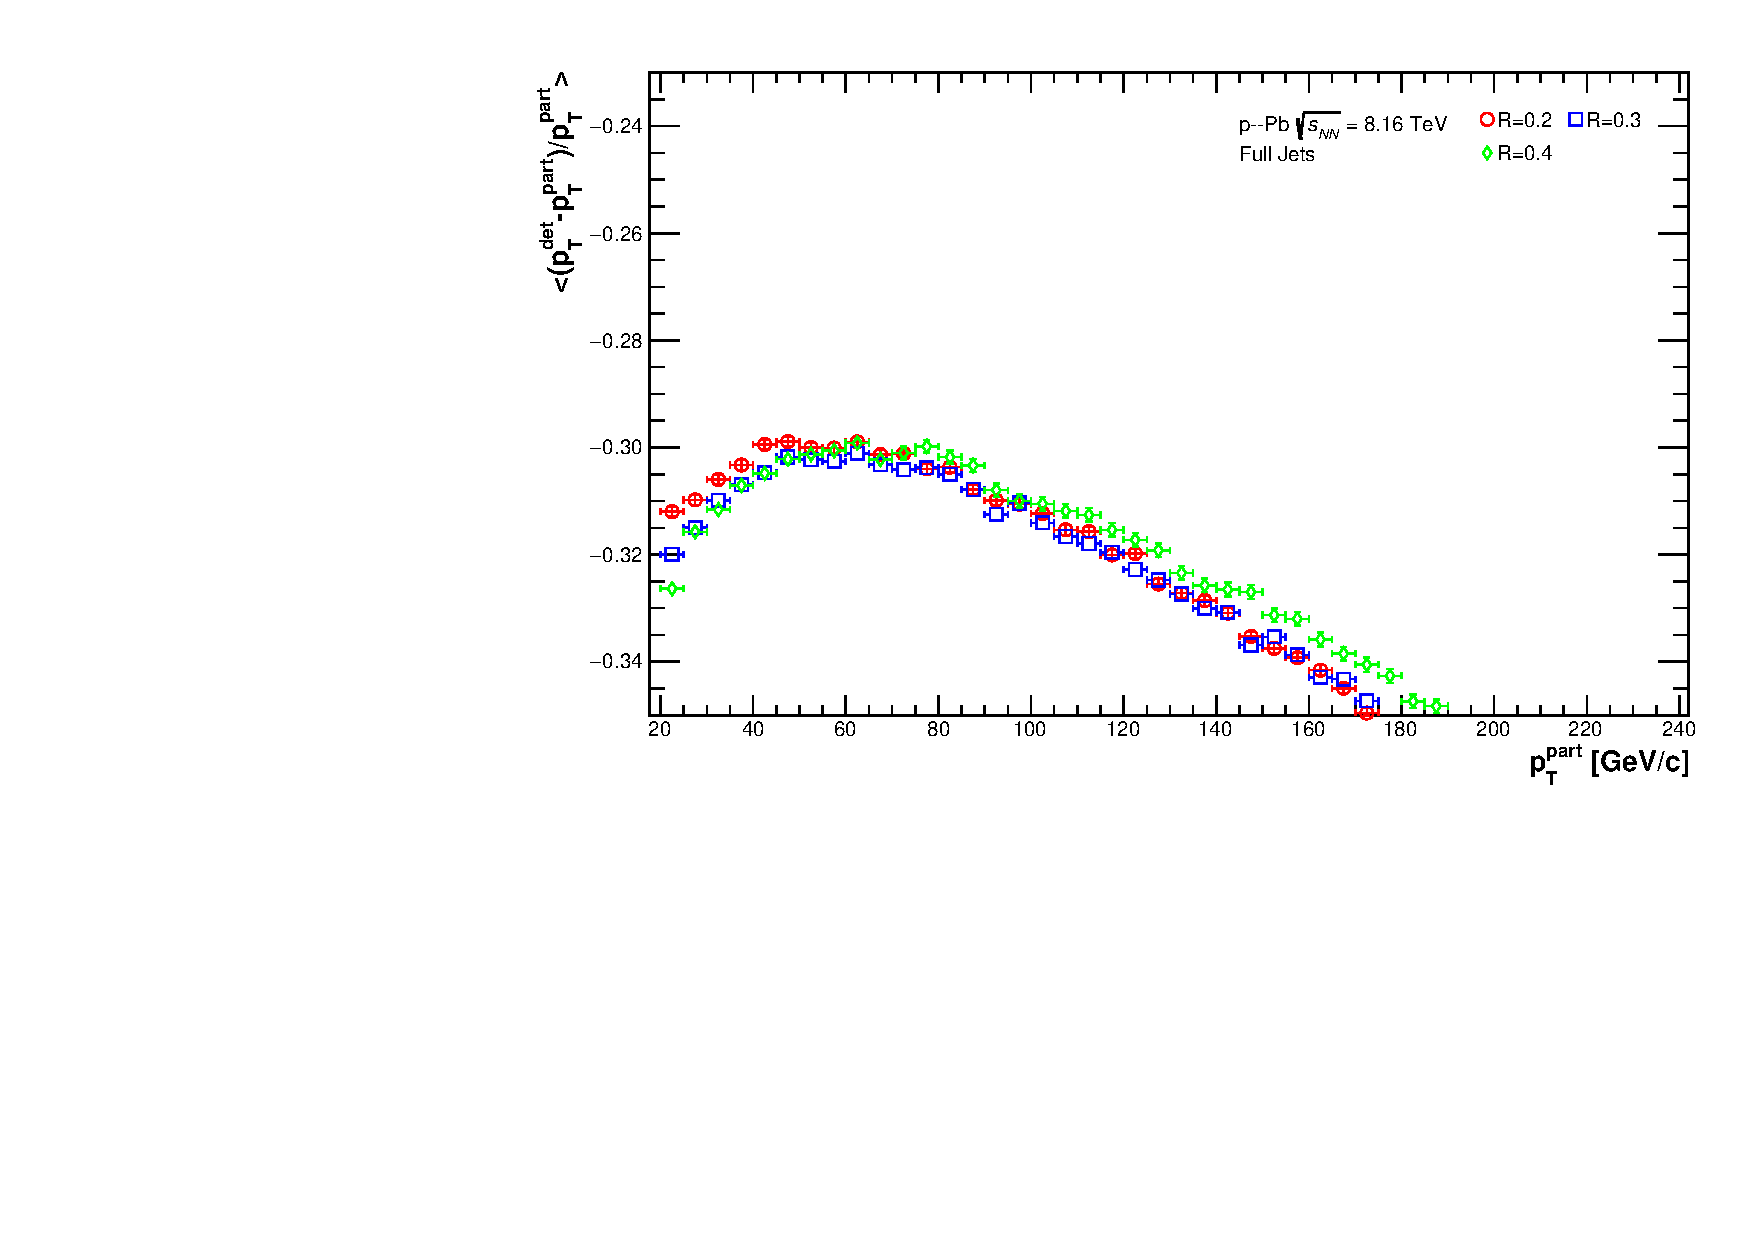
\includegraphics[width=0.49\textwidth]{figures/pPbFigures/EnergyScale/EnergyScaleMean.pdf}
    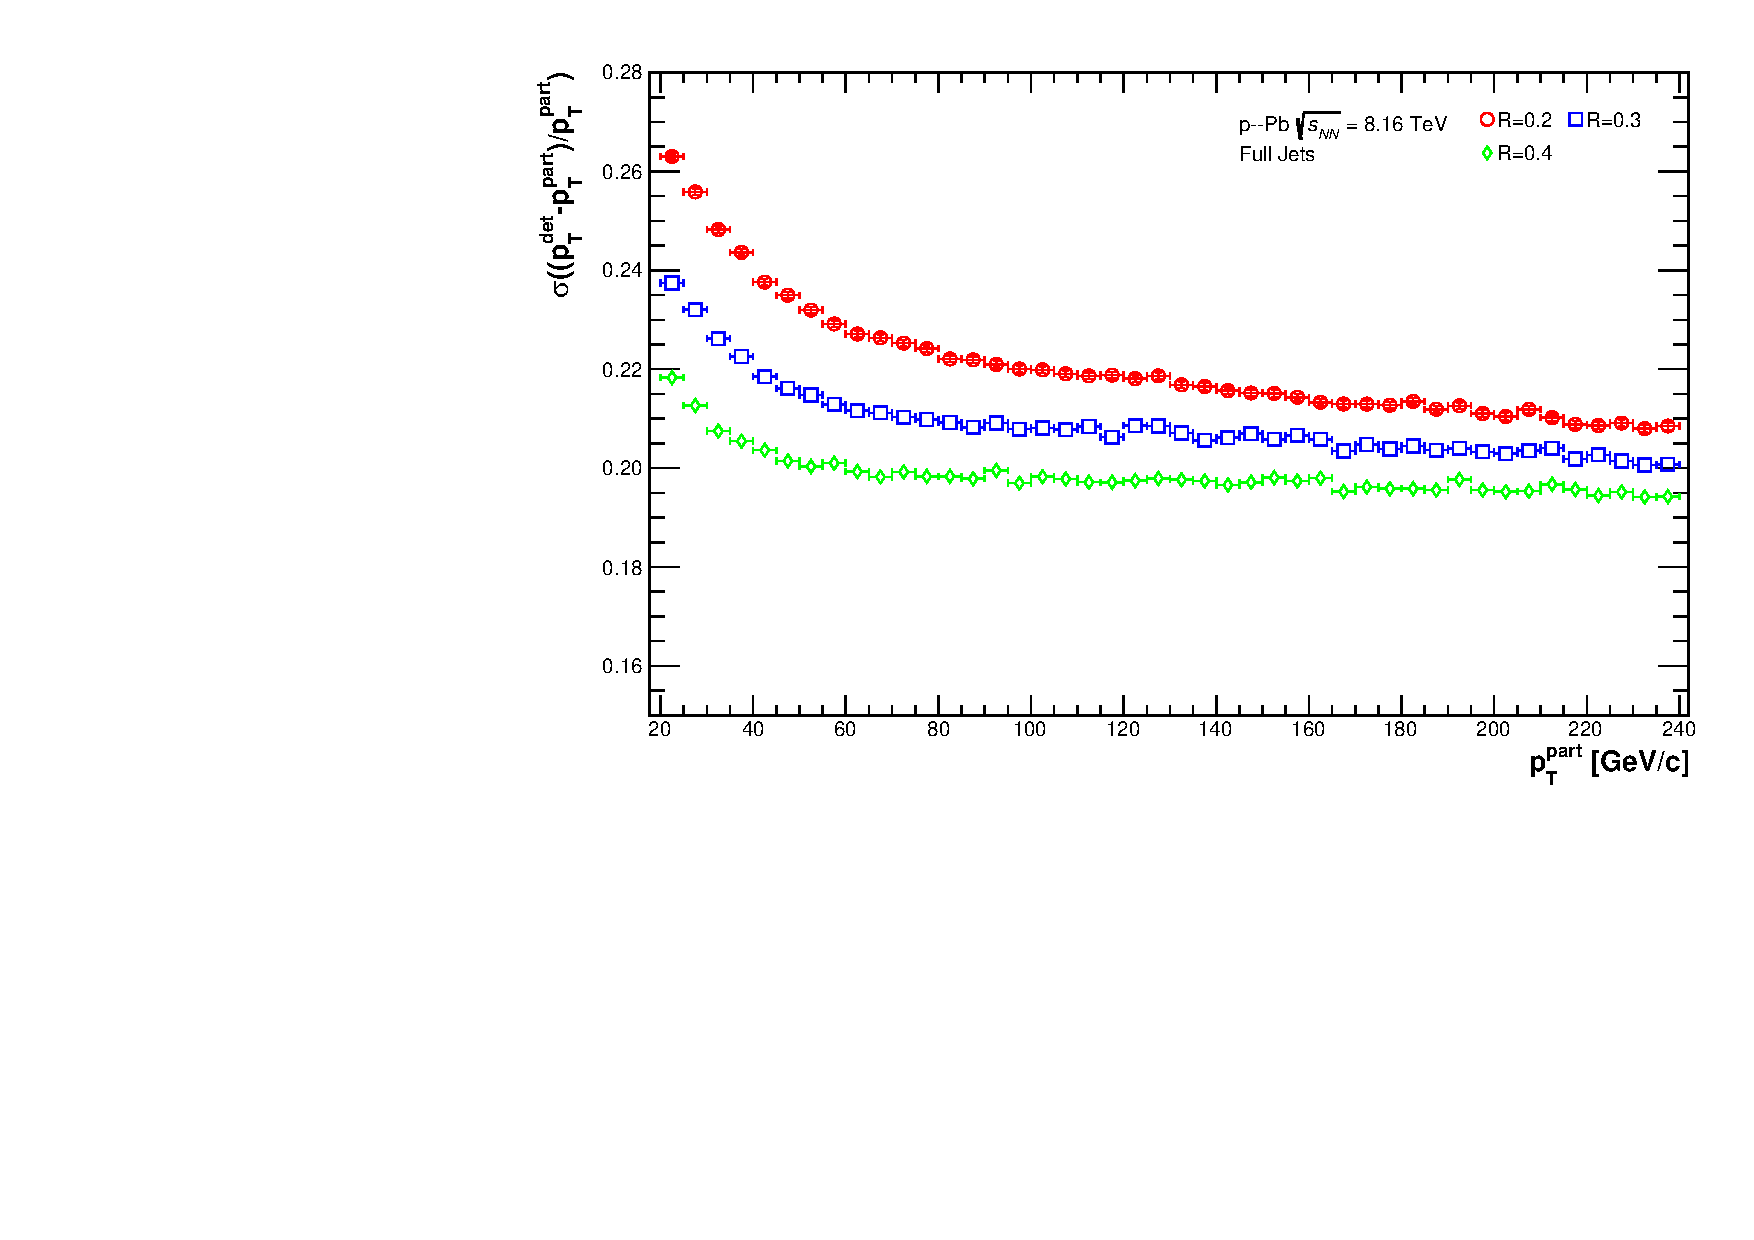
\includegraphics[width=0.49\textwidth]{figures/pPbFigures/EnergyScale/EnergyScaleWidth.pdf}
    \caption{Jet energy scale (left) and jet energy resolution (right) showing the instrumental response to jets in \pPb collisions.}
    \label{fig:EnergyScalepPb}
\end{figure}

For \pp, a comparison to the energy scale results from 13 TeV is also included and can be seen in Figure~\ref{fig:EnergyScaleComp}. The larger the jet resolution parameter, the larger the difference compared to 13 TeV. This is likely due to detector performance effects. The performance during collection of the 13 TeV dataset was significantly different in part from a better resolution due to the inclusion of TRD tracking in approximately 50\% of events. Additionally, there was a smaller fraction of bad channels in the EMCal for run 2. The improvement in jet energy resolution in 13 TeV is greatest at high-\pT. At low-\pT, the resolution overlaps between the two datasets other than in the largest resolution parameter reported.


\begin{figure}[hbt!]
    \centering
    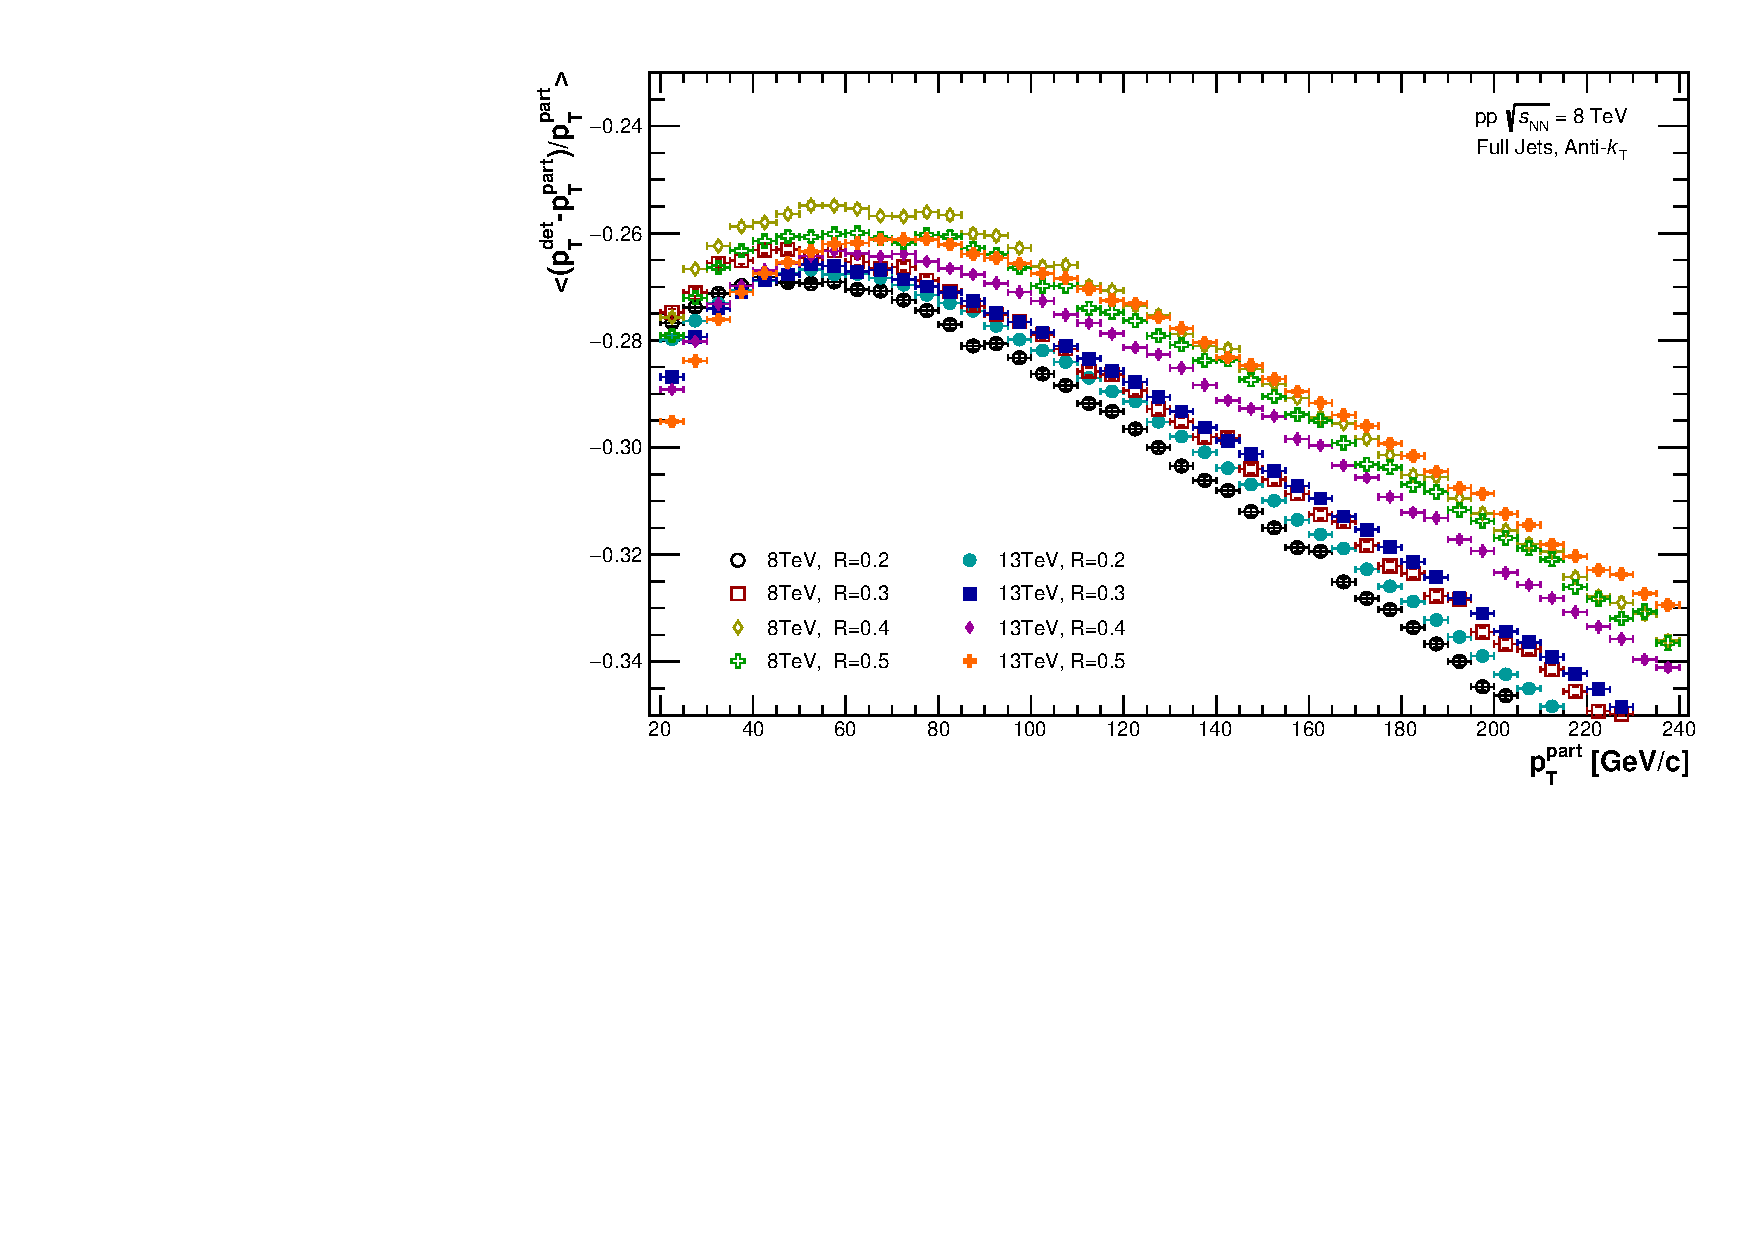
\includegraphics[width=0.49\textwidth]{figures/EnergyScale/EnergyScaleMean_Comparison.pdf}
    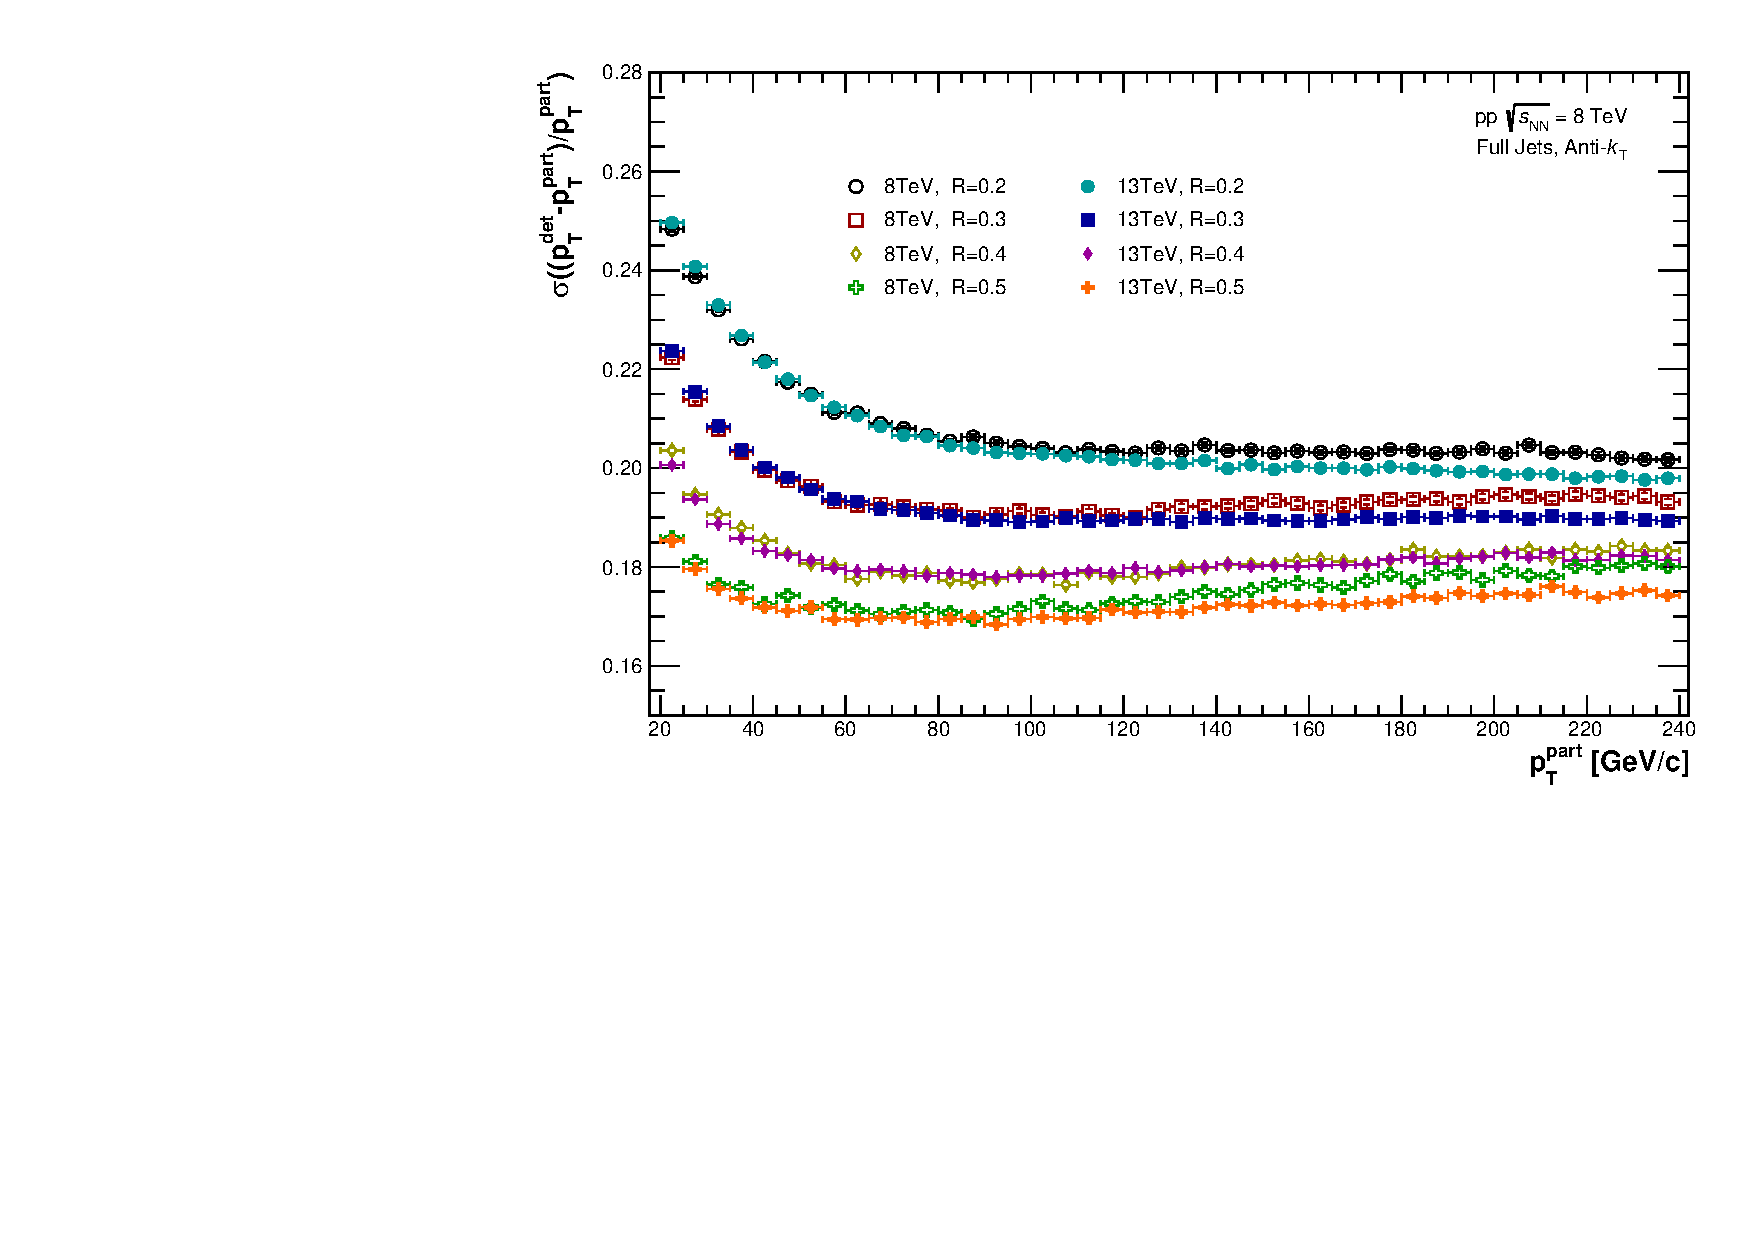
\includegraphics[width=0.49\textwidth]{figures/EnergyScale/EnergyScaleWidth_Comparison.pdf}
    \caption{Jet energy scale (left) and jet energy resolution (right) from the results of this analysis (\pp 8 TeV) compared to those of this analysis of data from \pp collisions at \s = 8 TeV compared to the analysis of jets from \pp collisions at \s = 13 TeV.}
    \label{fig:EnergyScaleComp}
\end{figure}

A different R-ordering can also be seen when comparing the jet energy scale from 8 TeV to that of 13 TeV. For 13 TeV, the energy scale increases with increasing radii from R = 0.2 to 0.6. In 8 TeV, the energy scale increases from R = 0.2 to 0.4, then decreases again for R = 0.5 and R = 0.6. Although the jet energy scale ordering is different, Figure~\ref{fig:eScaleShapeWidth} shows that the shape of the distributions is comparable, but energy resolution is slightly worse for 8 TeV.


\begin{figure}[hbt!]
    \centering
    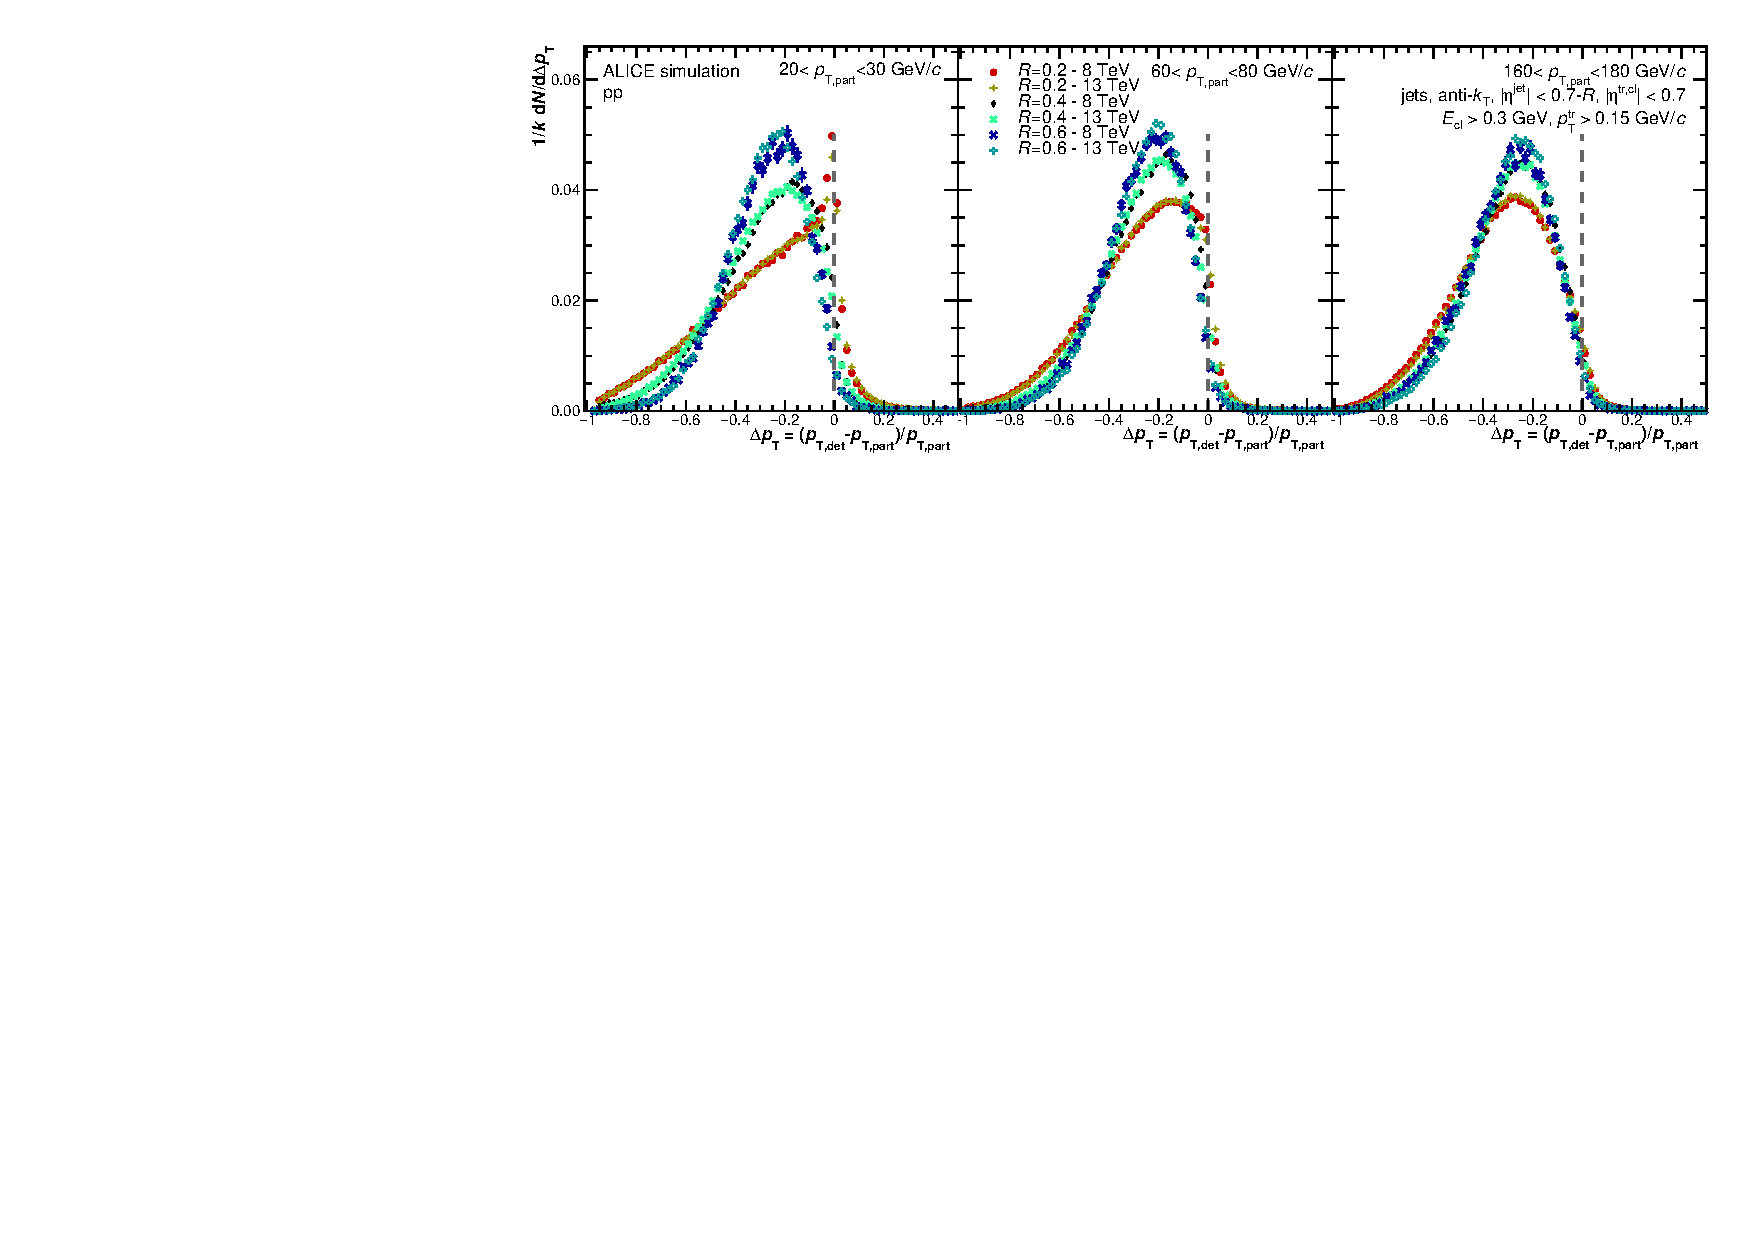
\includegraphics[width=\textwidth]{figures/EnergyScale/ROrdering/JetEscaleProj_3_EnergyComp.pdf}
    \caption{Jet energy scale projections showing the shape of the distributions for 8 and 13 TeV in \pp collisions.}
    \label{fig:eScaleShapeWidth}
\end{figure}

To explore the discrepancy, the jet energy scale is broken down into its charged track and EMCal cluster components, which will be referred to as the charged and neutral components, seen in Figure~\ref{fig:eScaleChNe}. The R-ordering difference is seen for both components, but is greater for the neutral component. In 2012, there was acceptance loss for the charged component due to dead areas in the SPD tracking, and the ITS-TPC track matching was different as a function of $\phi$. Charged particles that pass through these areas will not result in SPD clusters, and thus will not produce an SPD tracklet. The larger the jet resolution parameter, the more likely it is for tracks contained within the jet cone to overlap with these dead areas. The more a jet overlaps with dead areas, the greater the difference between particle and detector level. This effect was not present for the majority of the runs, which is evident by the smaller impact compared to the neutral component. The neutral component is also impacted by the partially installed TRD in 2012. Some of the EMCal supermodules had TRD material in front of them, while others did not. The larger the jet resolution parameter, the more likely it was to cross boundaries in the EMCal between where there was and was not TRD material. As is the case for the dead areas of the SPD, jets overlapping with the TRD will have less of the jet energy reconstructed at detector level. Example plots showing tracking and EMCal occupancy as a function of $\eta$ and $\phi$ can be seen in Figure~\ref{fig:eScaleTracksClusters}. The R-ordering effect observed for \pp collisions at 8 TeV is not seen for \pPb collisions at 8.16 TeV. The \pPb data were recorded during run 2 and benefit from the same improved detector conditions as \pp collisions at 13 TeV.


\begin{figure}[hbt!]
    \centering
    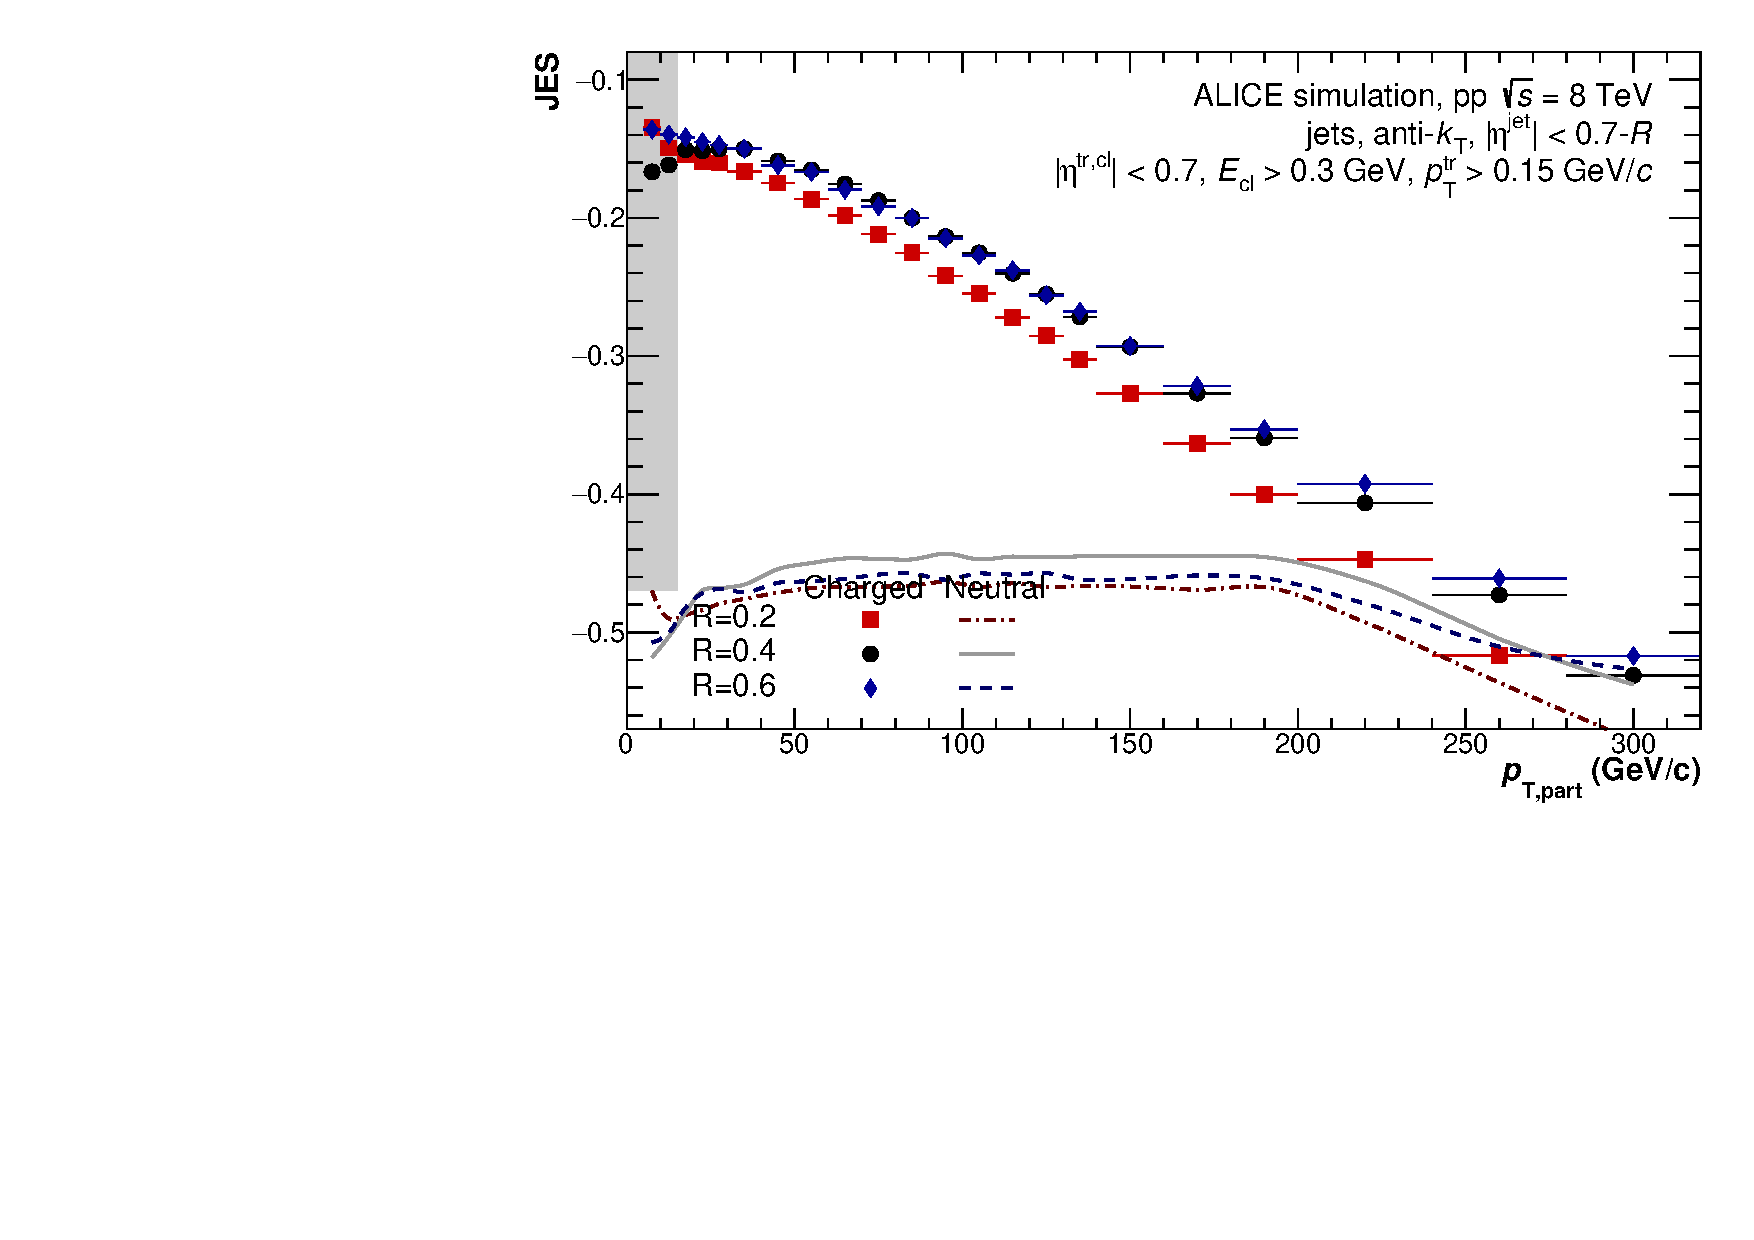
\includegraphics[width=0.75\textwidth]{figures/EnergyScale/ROrdering/JES_8_3_ChNe.pdf}
    \caption{Jet energy scale broken up into its charged and neutral components.}
    \label{fig:eScaleChNe}
\end{figure}


\begin{figure}[hbt!]
    \centering
    %\subfigure{
        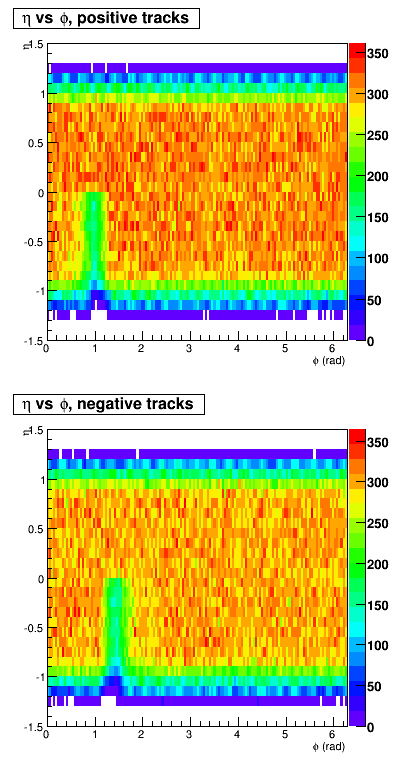
\includegraphics[width=0.35\textwidth]{figures/EnergyScale/ROrdering/spd_holes.png}
    %}
    %\subfigure{
        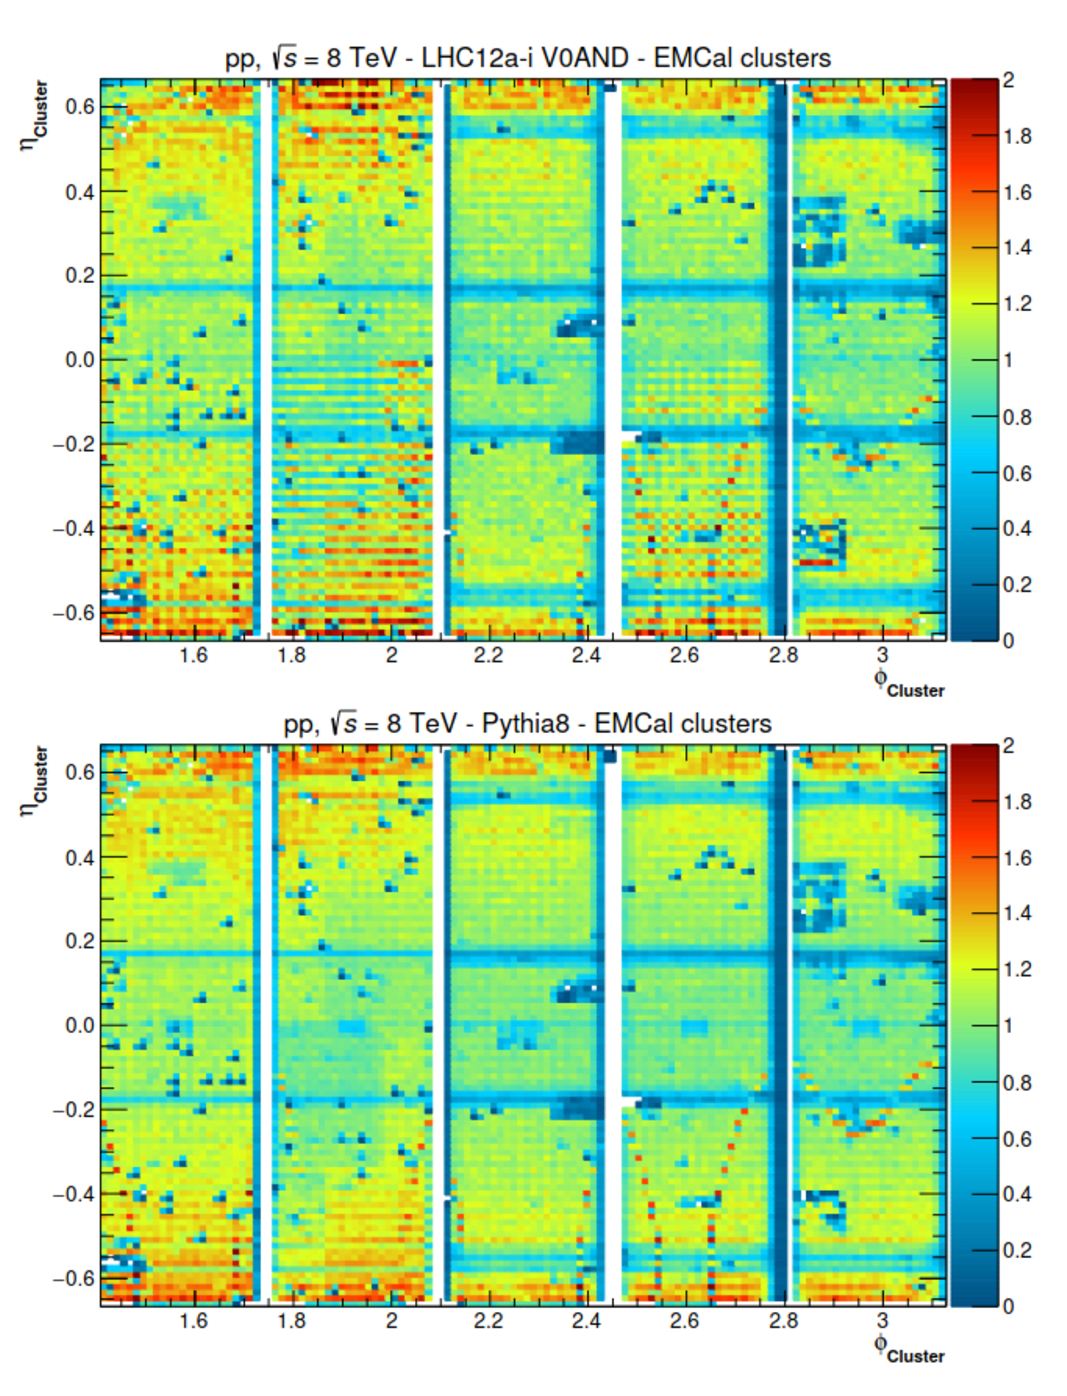
\includegraphics[width=0.5\textwidth]{figures/EnergyScale/ROrdering/emcal_occupancy_cropped.eps}
    %}
    \caption{TPC-ITS track distribution (left) and EMCal cluster distribution (right) as a function of $\eta$ and $\phi$. The top right plot shows the EMCal cluster distribution for the V0AND minimum bias trigger in the 2012 dataset, while the bottom right plot shows the EMCal cluster distribution for the same dataset modeled by PYTHIA8 propagated though a GEANT simulation of the detector.}
    \label{fig:eScaleTracksClusters}
\end{figure}

\subsection{Kinematic efficiency}
\label{sec:kinEff}


\begin{figure}[hbt!]
    \centering
    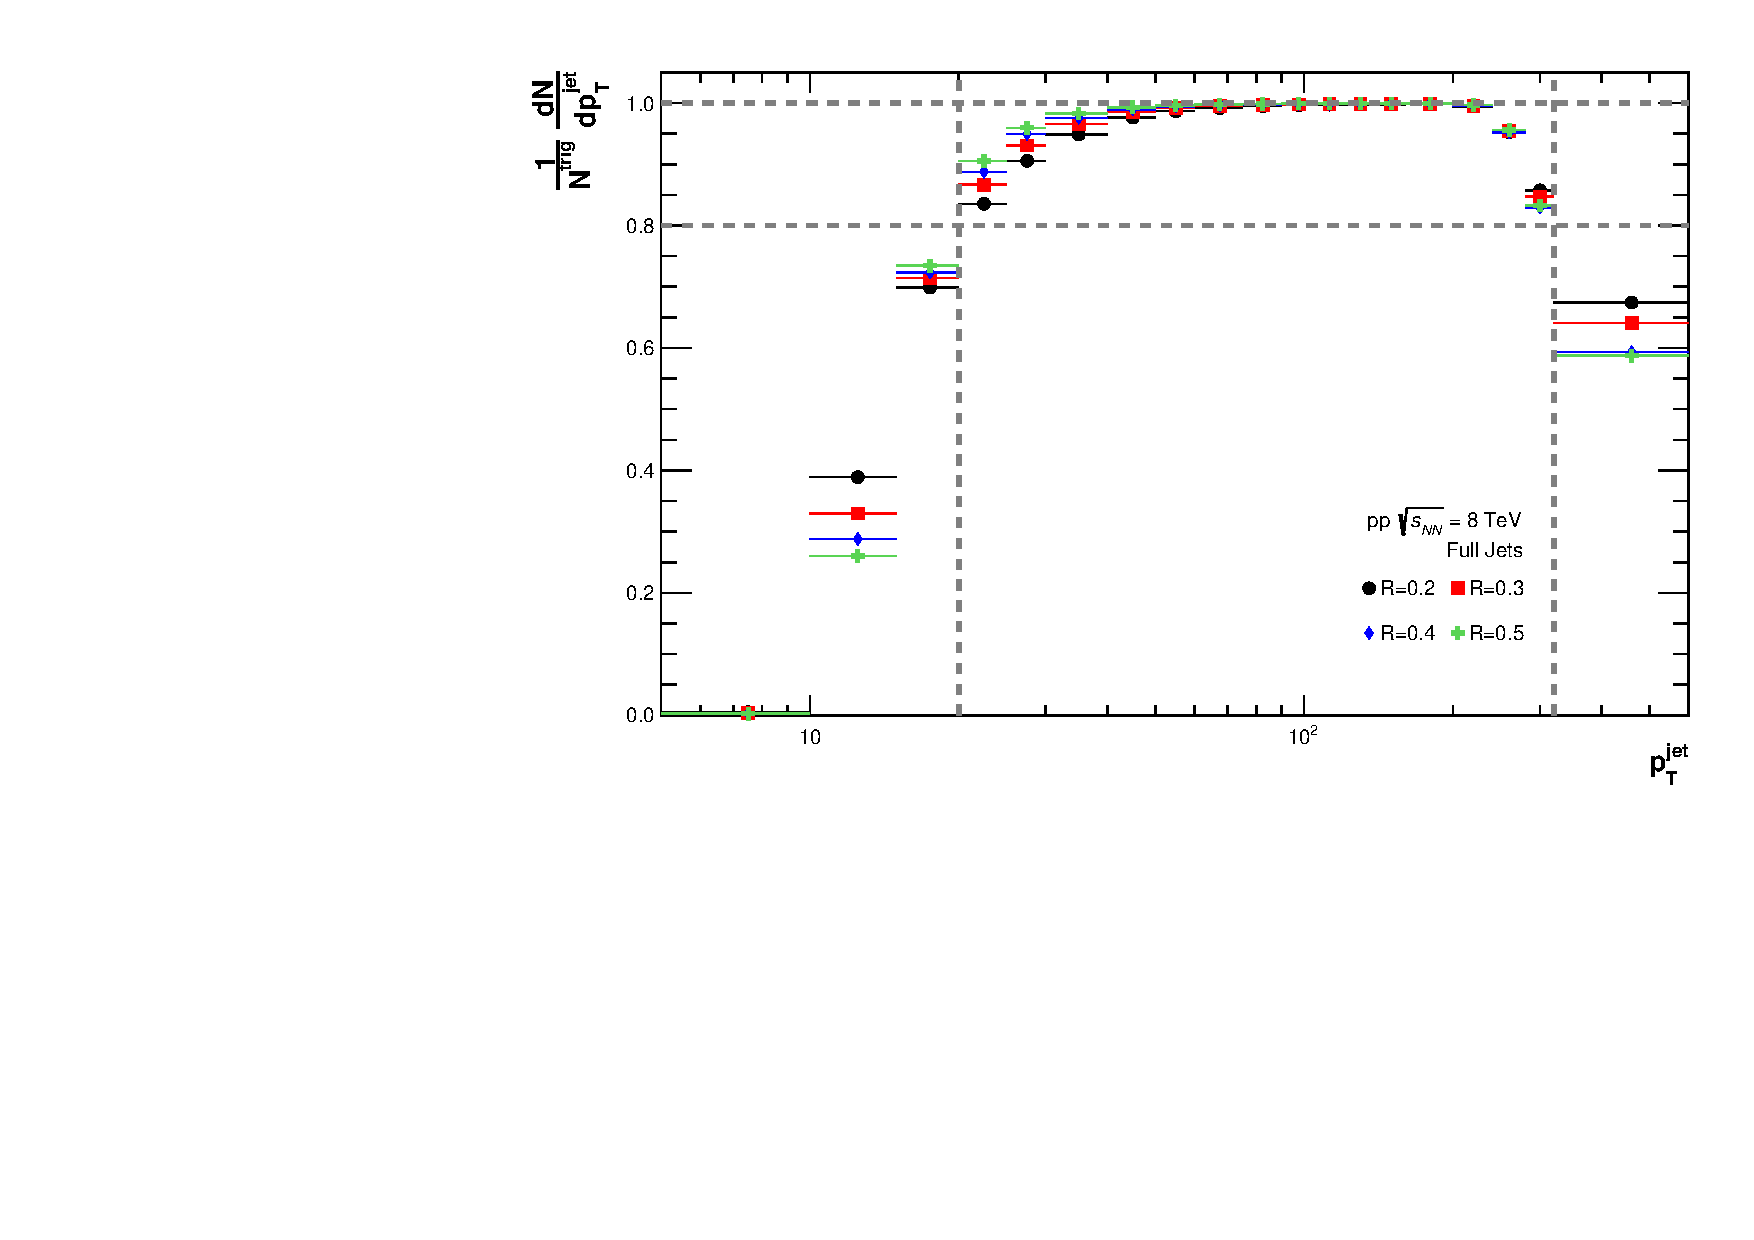
\includegraphics[width=15cm]{figures/KinematicEfficiency/EffKine.pdf}
    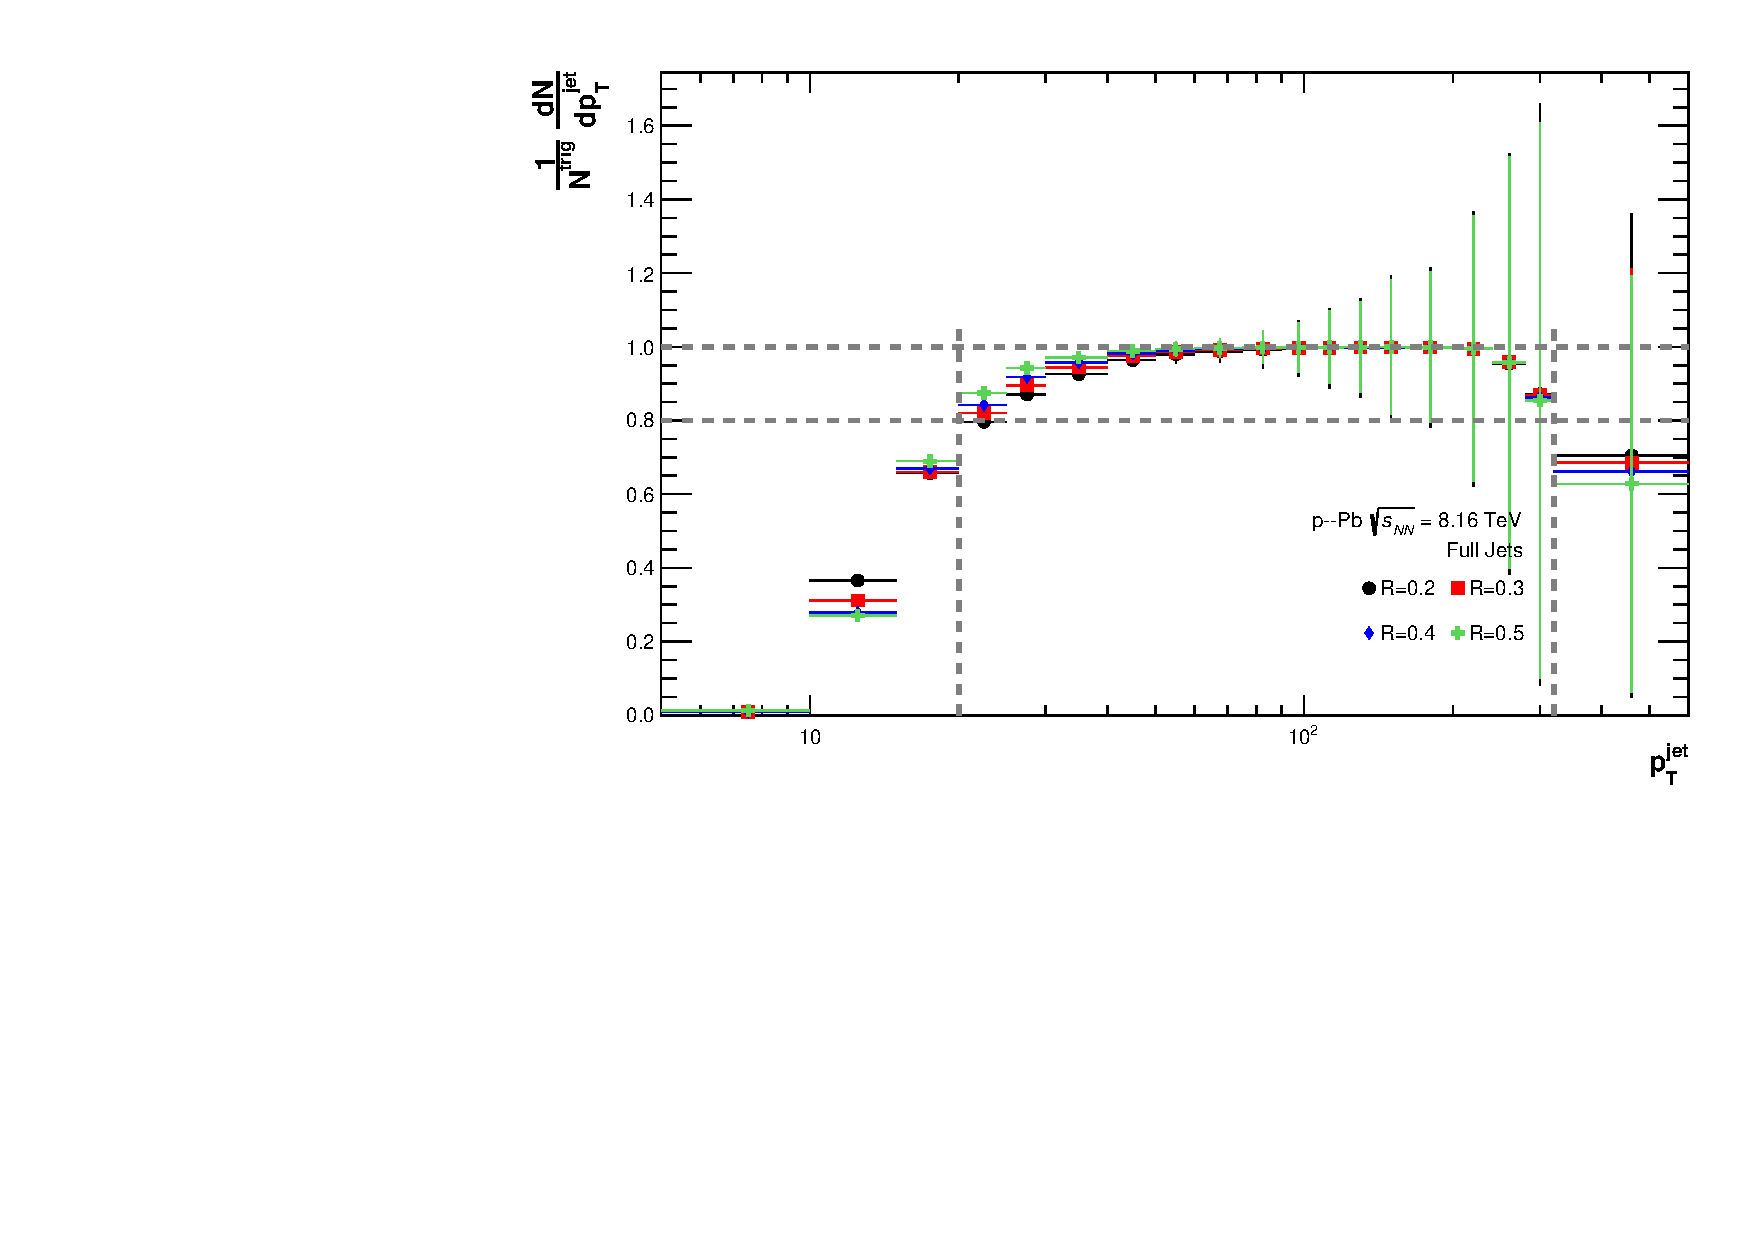
\includegraphics[width=15cm]{figures/pPbFigures/KinematicEfficiency/EffKine.pdf}
    \caption{Kinematic efficiency for various jet radii in \pp (top) and \pPb (bottom).}
    \label{fig:KinematicEfficiency}
\end{figure}

The kinematic efficiency is the fraction of particle level jets matched to jets which are reconstructed at detector level. Truncating the response matrix at low and high \pT at detector level causes some jets at particle level to be lost because they fall outside the chosen range. By dividing by the kinematic efficiency, the spectrum is corrected for jets that were reconstructed but did not pass the matching criteria, i.e. jets that were not matched between particle and detector level because they fell outside the selected \pT range or detector acceptance. The kinematic efficiency is found by taking a projection of the response matrix over the selected detector range relative to the full range. The kinematic efficiency must be at least 80$\%$ in order to ensure each bin is well constrained by data. Low percentages suggest that the jets in that kinematic range would need to be heavily corrected by unfolding and are thus highly dependent on PYTHIA. The choice of 80$\%$ was determined by ALICE to be within a range that is constrained sufficiently by data.

Figure~\ref{fig:KinematicEfficiency} shows the kinematic efficiency for jets with R = 0.2 to R = 0.6 for \pp and R = 0.2 to R = 0.5 for \pPb. Jets are selected at detector level to have a \pT within 10 and 240 GeV/$c$. The efficiency is 80$\%$ beyond 20 GeV/$c$, and stays around this value in the whole region covered by the measurement. At lower \pT, the turn-on is sharper for jets with larger jet radii. A measurement is feasible for 20 GeV /c $<$ \pT $<$ 320 GeV/$c$ where the kinematic efficiency is larger than 80$\%$.

\subsection{Unfolding of the jet spectrum}
\label{sec:unfolding}

For this measurement, both Bayesian unfolding and unfolding based on singular value decomposition (SVD) are used to correct the spectrum. Both methods were implemented in the RooUnfold framework \cite{roounfold}. The Bayesian method is used as the standard method, while SVD unfolding is used to test the sensitivity with respect to different unfolding methods. The unfolding process must be dealt with carefully due to several assumptions made. First, it is assumed that the true spectrum has a similar shape to the Monte Carlo spectrum used to create the detector response. Second, the assumption is made that a jet reconstructed at detector level corresponds to a jet reconstructed at truth level. These assumptions can lead to biases in the results. Several tests are performed to minimize the impact of these biases on the final spectrum.

Bayesian unfolding, introduced by D'Agostini~\cite{D'Agostini:265717}, is an iterative process to find the best estimate for true spectrum from the raw spectrum. The raw spectrum refers to the jet spectrum after scaling correction but before unfolding, as in Equation~\ref{eq:corrraweq}. This process can be expressed in terms of causes C, representing the true spectrum, and effects E, representing the raw spectrum. Each cause can impact multiple effects, and the exact cause for a given effect is not known. Bayes theorem is then given by the equation

\begin{equation}
    P(C_i|E_j) = \frac{P(E_j|C_i)\cdot P_0(C_i)}{\Sigma_l^{n_C}P(E_j|C_l)\cdot P_0(C_l)}
\end{equation}

\noindent
where $P(C_i|E_j)$ is the probability that a cause is responsible for a specific effect, $P(E_j|C_i)$ is the probability of having an effect produced from a defined cause, and $P_0(C_i)$ is the prior or initial probability of causes. $P(E_j|C_i)$ can also be thought of as the distribution of migration probabilities, or the probability of a cause migrating to a given effect. This can be thought of as a jet of a certain true momentum being reconstructed at some other momentum. The expected number of events for a given cause representing the true spectrum is then given by

\begin{equation}
    \hat{n}(C_i) = \frac{1}{\epsilon_i}\Sigma_{j=1}^{n_E}n(E_j)\cdot P(C_i|E_j), \; \epsilon_i \neq 0
\end{equation}

\noindent
where $\epsilon_i$ is the efficiency of a cause producing an effect, and $n(E_j)$ is the number of events for a given effect representing the measured or smeared spectrum. This equation can be rewritten in terms of the response matrix as

\begin{equation}
    \hat{n}(C_i) = \Sigma_{j=1}^{n_E}M_{ij}\cdot n(E_j)
\end{equation}

\noindent
where the response matrix is

\begin{equation}
    M_{ij} = \frac{P(E_j|C_i)\cdot P_0(C_i)}{[\Sigma_{l=1}^{n_E}P(E_l|C_i)] \cdot [\Sigma_{l=1}^{n_C}P(E_j|C_l)\cdot P_0(C_l)]}
\end{equation}

\noindent
Due to the iterative nature of the Bayesian process, a perfect prior knowledge of the behavior of the true spectrum is not required. The prior can be chosen to be flat or uniform, and a satisfactory result can still be reached. The prior is typically taken from Monte Carlo simulations and is taken from PYTHIA in this instance because it gets most aspects of the spectrum correct. The closer the prior is to the true spectrum, the better the outcome will be. To iterate using the Bayesian process, the prior is replaced by the new "true" spectrum, and the process is repeated until the spectrum converges. 

Unfolding using the SVD method was first introduced by Hocker and Kartvelishvili~\cite{Hocker:1995kb}. This method again begins with the relationship between the true spectrum x and the raw spectrum b, given by

\begin{equation}
    \hat{A}x = b
\end{equation}

\noindent
where $\hat{A}$ is the response matrix. The response matrix is then decomposed into three matrices, $U$, $S$, and $V$ as 

\begin{equation}
    \hat{A} = U \cdot S \cdot V^T
\end{equation}

\noindent 
where U is an $m \times m$ orthogonal matrix, V is an $n \times n$ orthogonal matrix, and S is an $m \times n$ diagonal matrix of singular values. By swapping rows of the orthogonal matrices, the singular values can be ordered from largest to smallest. The inverse of the response matrix is easier to perform on the decomposed matrix, since S is diagonal, and the inverse of an orthogonal matrix is its transpose. The original system is 

\begin{equation}
    USV^Tx = b
\end{equation}

\noindent
Introducing vectors $z = V^Tx$ and $d = U^Tb$, the solution is given by

\begin{equation}
    z_i = \frac{d_i}{s_i}, \; x = Vz
\end{equation}

\noindent 
Two issues can arise with this solution. The first is that the singular values can be very small or zero, which can lead to large fluctuations in the solution. The second is that $d_i$ can be poorly known or insignificant. Inspecting the exact solution $z_i$ as a function of $|d_i|$, also known as the D-vector, shows that at high enough i values of $|d_i|$, changes to the solution are insignificant. A regularization parameter $k$ is introduced to the solution in the form 

\begin{equation}
    z_i^{(k)} = \frac{d_i}{s_i}\cdot \frac{s_i^2}{s_i^2 + s_k^2}
\end{equation}

\noindent
where k should be chosen to be the index of the last significant d. If k is chosen to be too small, the solution will be dominated by the prior. If it is too large, the solution will be dominated by high frequency statistical fluctuations.

The following figures contain unfolding test results for jet resolution parameter R = 0.2 for SVD and Bayesian unfolding to ensure stability of the unfolding process (for the remaining jet radii, see Appendix~\ref{sec:AppendixUnfoldingTests}). The goal of performing these tests is to find convergence of the jet spectra with increasing regularizations or iterations of the unfolding procedure.


\begin{figure}[hbt!]
    \centering
    \begin{multicols}{2}
            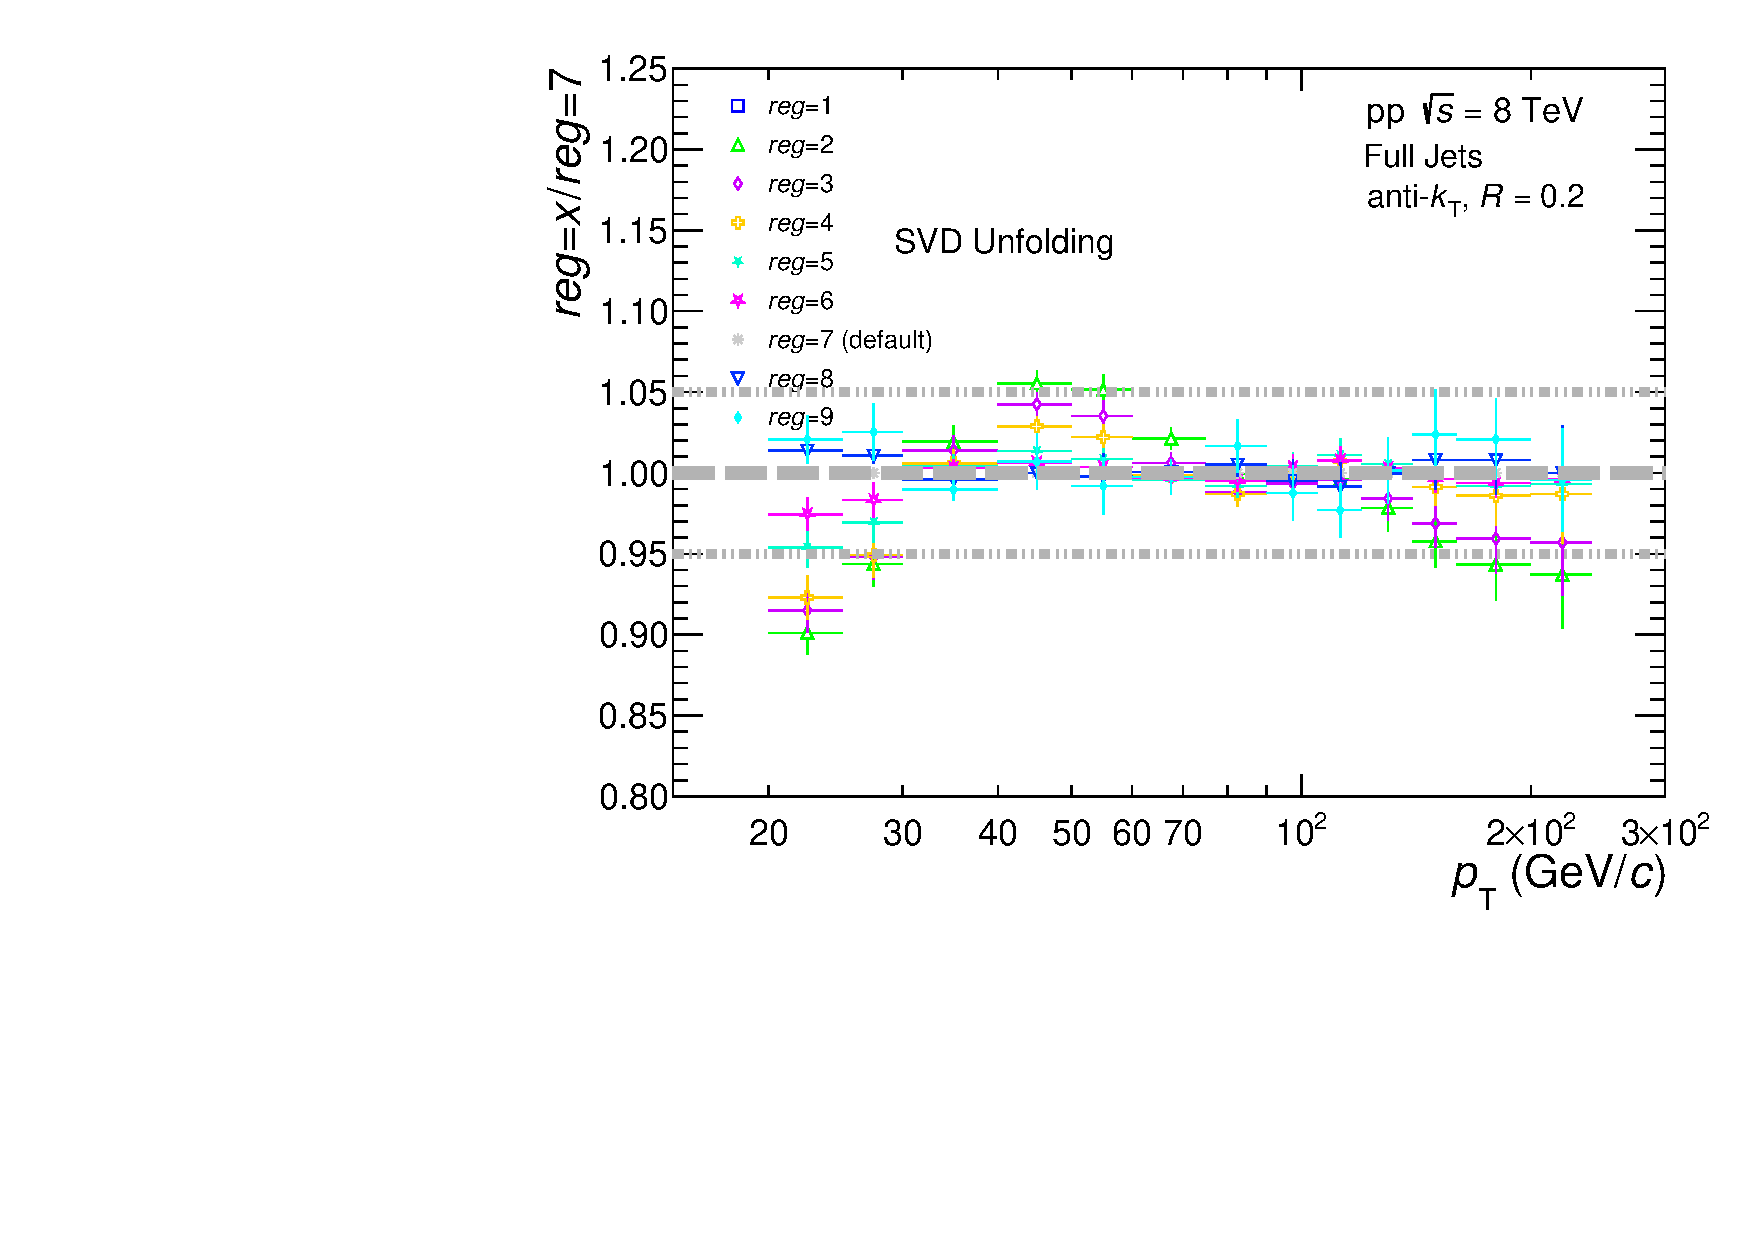
\includegraphics[width=0.49\textwidth]{figures/UnfoldingComparisons/Regularizations/RatioRegularizationSvd_R02.pdf}
        \vfill\null 
        \columnbreak
            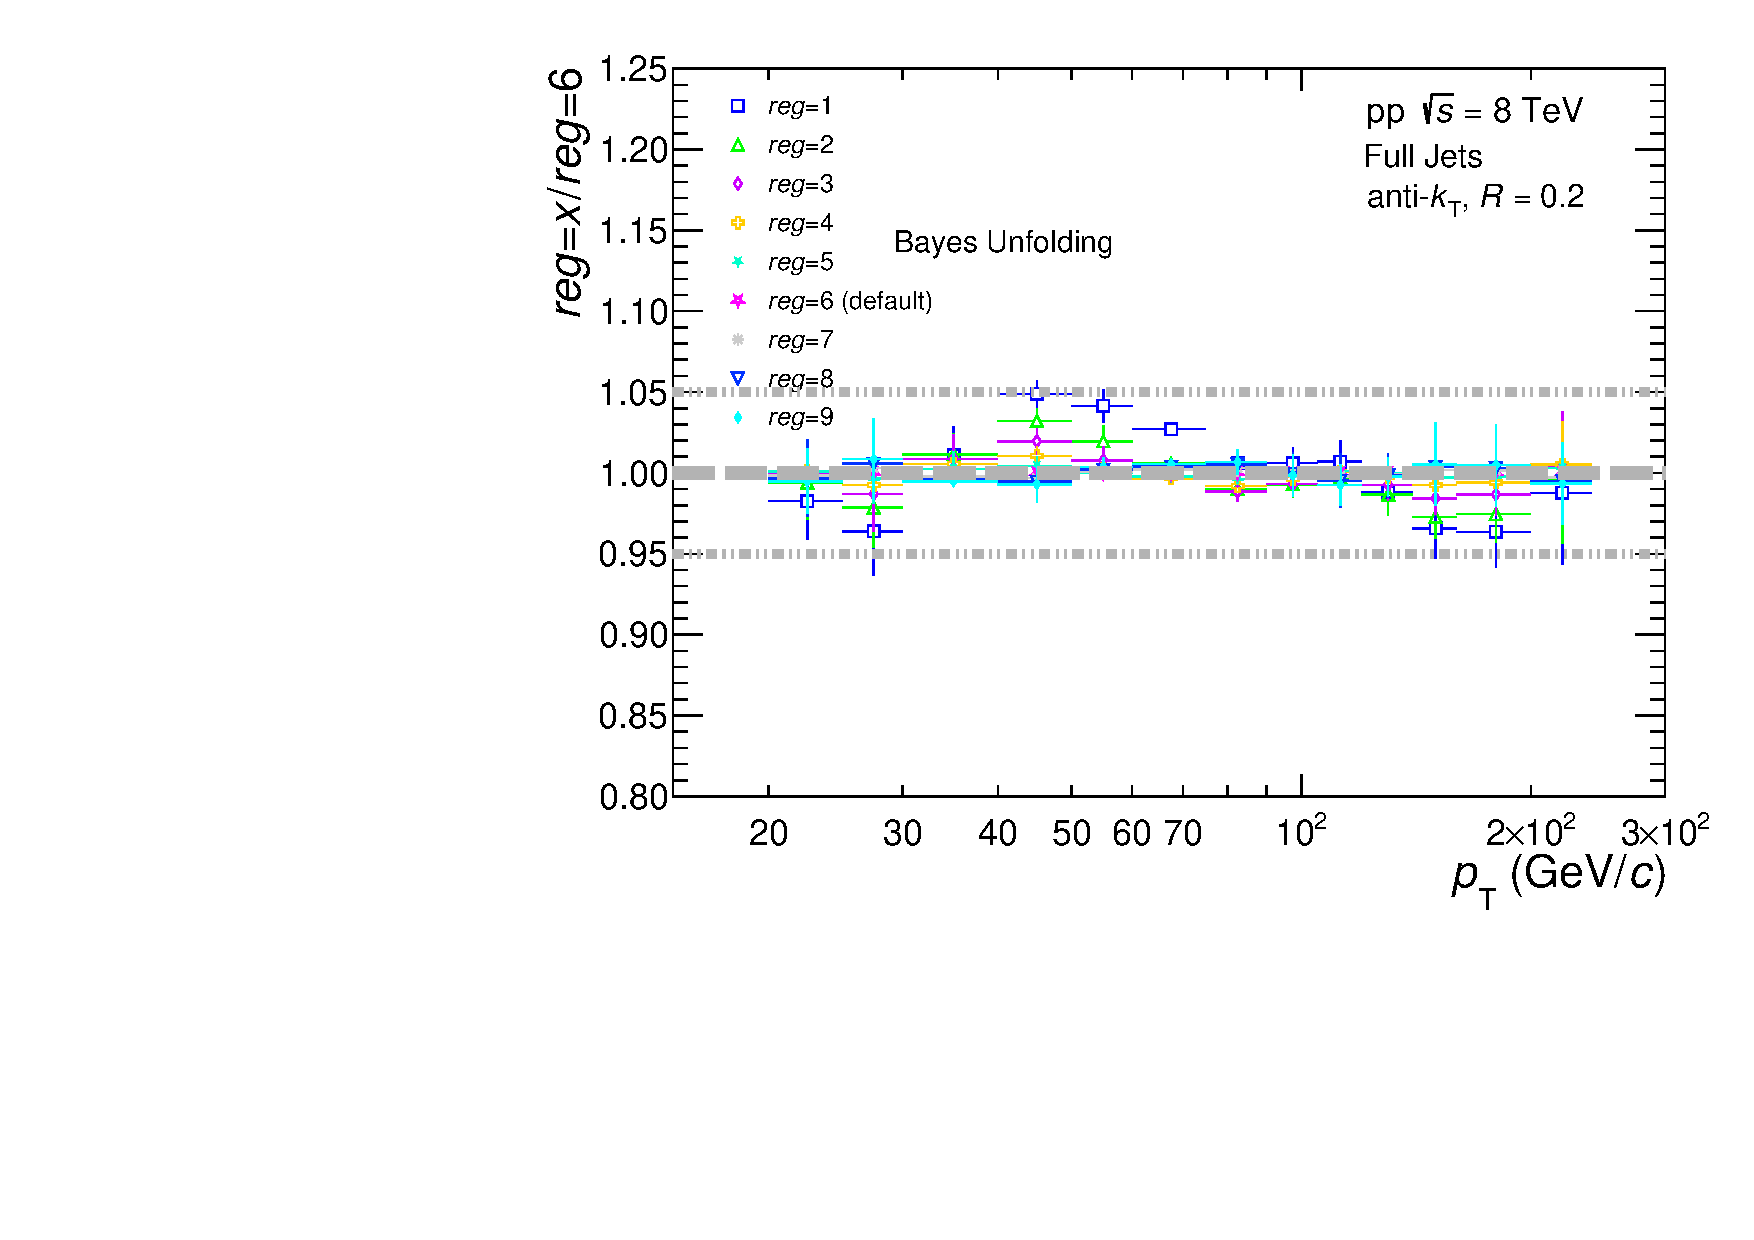
\includegraphics[width=0.49\textwidth]{figures/UnfoldingComparisons/Regularizations/RatioRegularizationBayes_R02.pdf}
        \vfill\null
    \end{multicols}
    \caption{Regularization dependence for SVD (left) and iterations of Bayesian (right) unfolding of jets in \pp collisions. Iterations are also labeled as "reg" in this plot for visual comparison between the methods.}
    \label{fig:RegIter}
\end{figure}


Figure~\ref{fig:RegIter} shows the dependence of the SVD and Bayesian unfolded solutions on the regularization parameter and number of iterations, respectively. A regularization parameter of 7 is selected as default for the SVD unfolding, while 6 iterations are chosen as default for Bayesian unfolding with 4 and 9 iterations as variations. The choice of the regularization parameter for SVD of 7 is also motivated by the D-vector, shown in Figure~\ref{fig:DVector}. At low values of regularization parameter, the D-vector falls steeply. Changes in this regime are statistically significant. When the D-vector reaches a plateau, the spectrum no longer changes significantly with further regularizations. The default solution is chosen in this region. With increasing regularizations or number of iterations, the spectrum must at some point no longer change significantly and converge on a default solution.


\begin{figure}[hbt!]
    \centering
    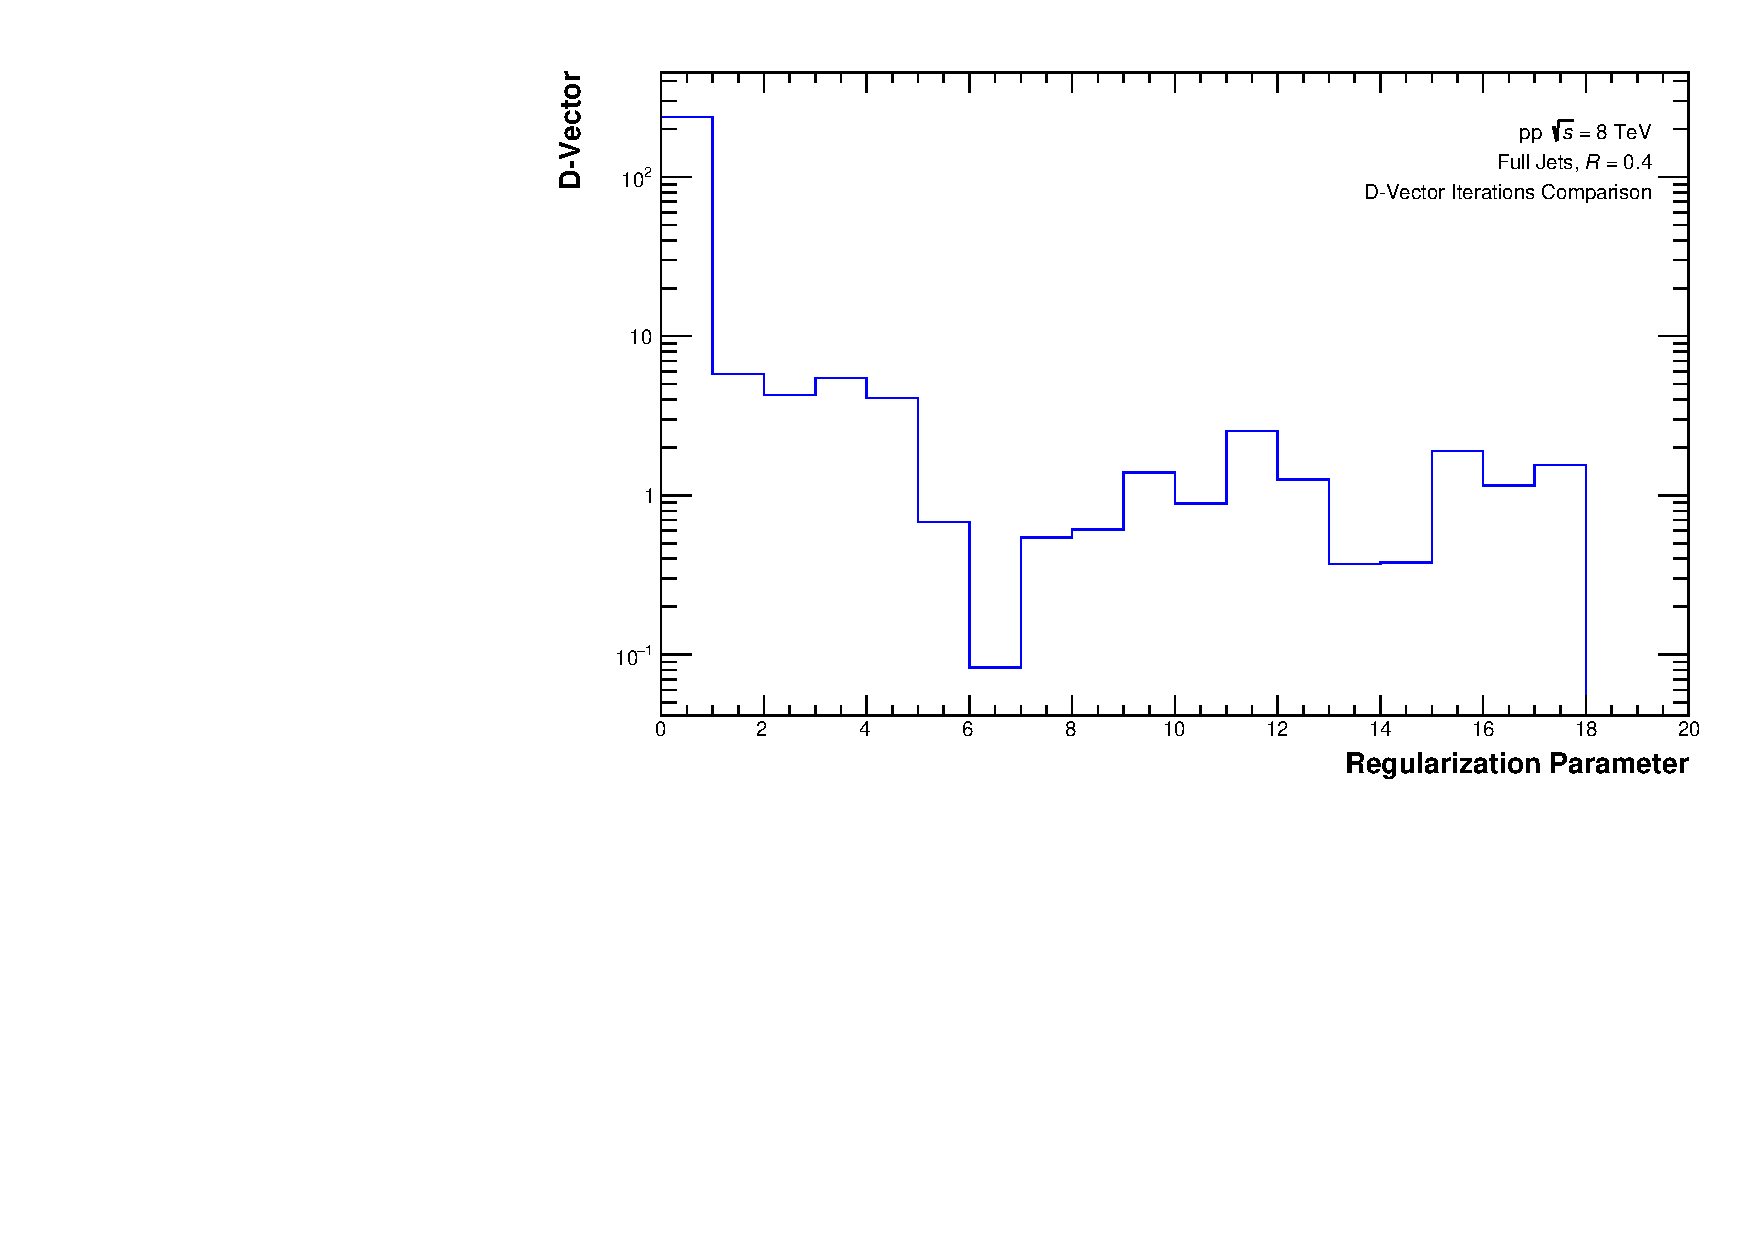
\includegraphics[width=15cm]{figures/DVector/DVector_R04.pdf}
    \caption{D-Vector comparison for multiple regularizations of SVD unfolding of the jet spectrum for $R$ = 0.4 in \pp collisions.}
    \label{fig:DVector}
\end{figure}


\begin{figure}[hbt!]
    \centering
    \begin{multicols}{2}
        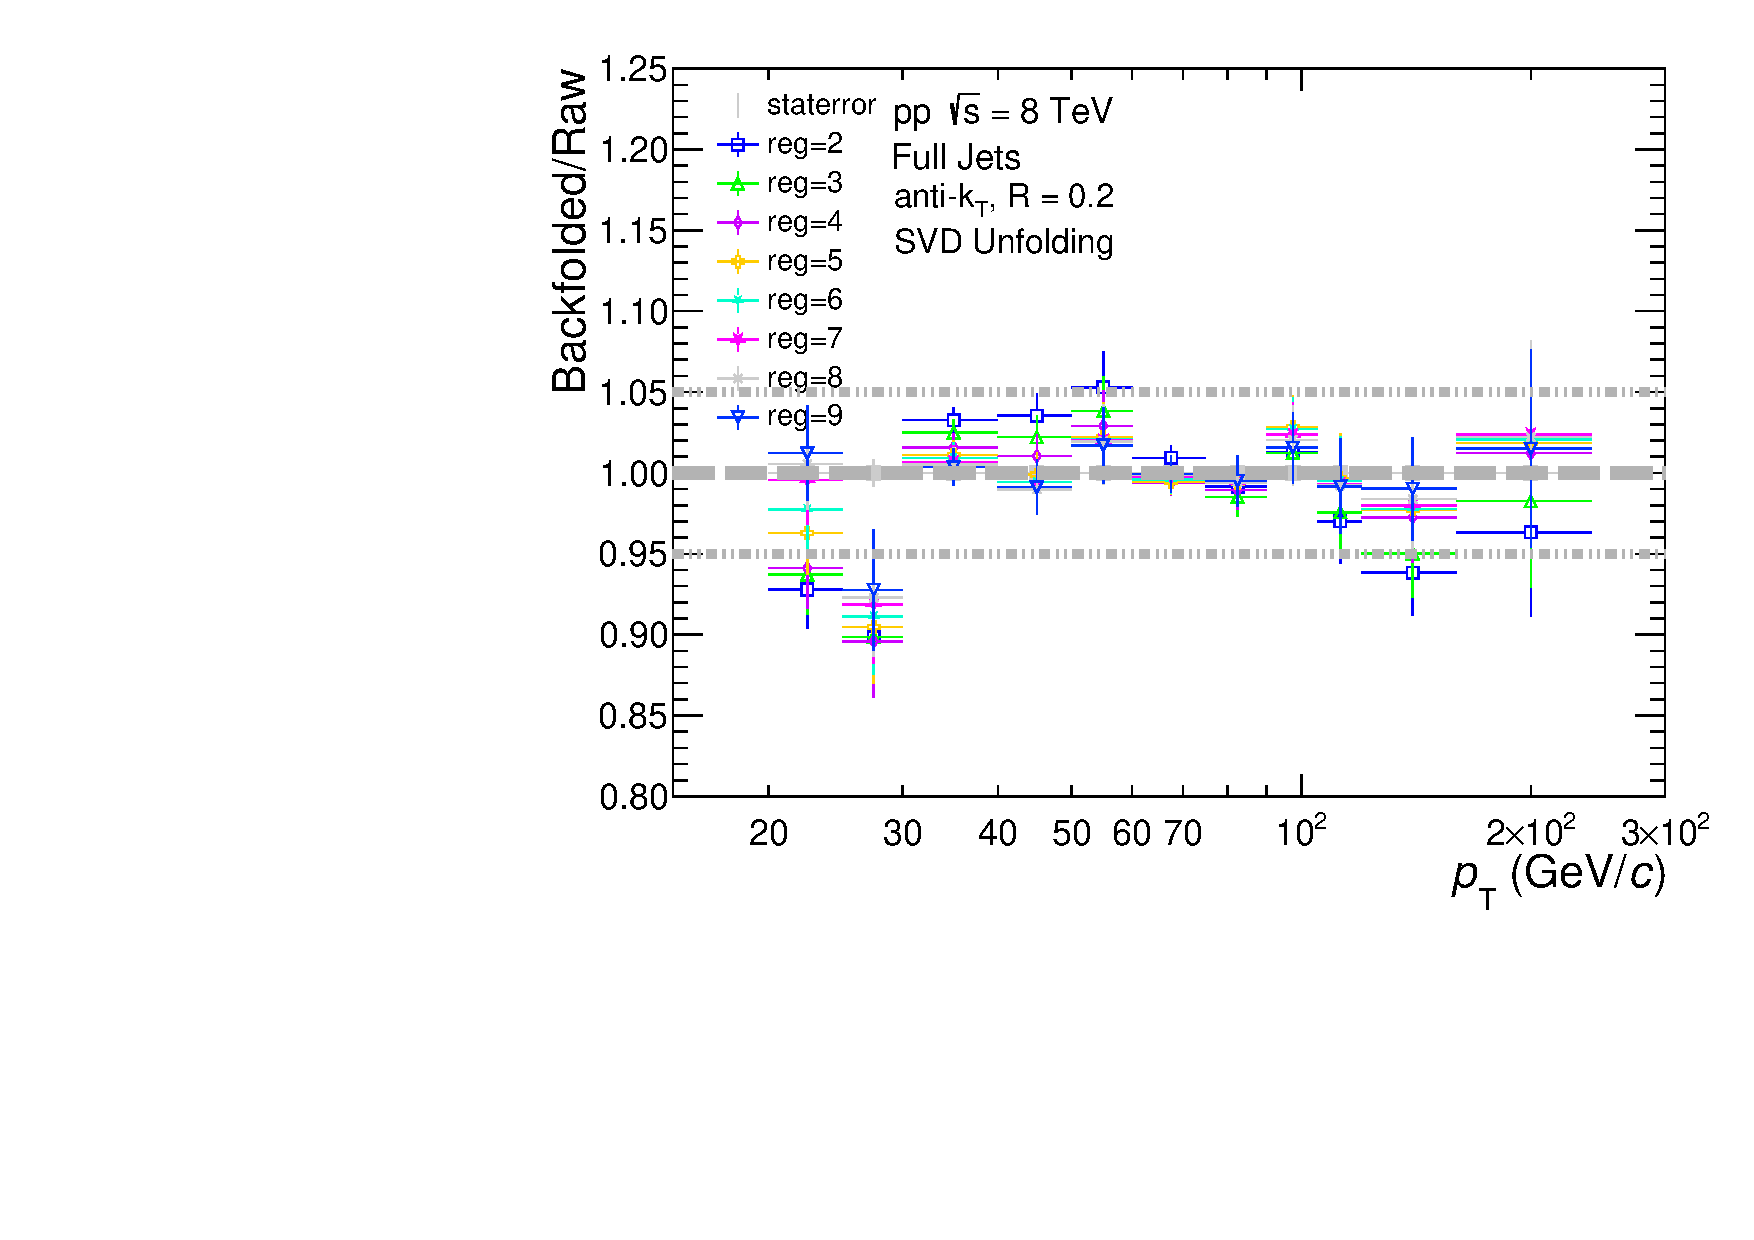
\includegraphics[width=0.49\textwidth]{figures/UnfoldingComparisons/BackfoldedVsRaw/RatioFoldRawSvd_R02.pdf}
    \vfill\null
    \columnbreak
        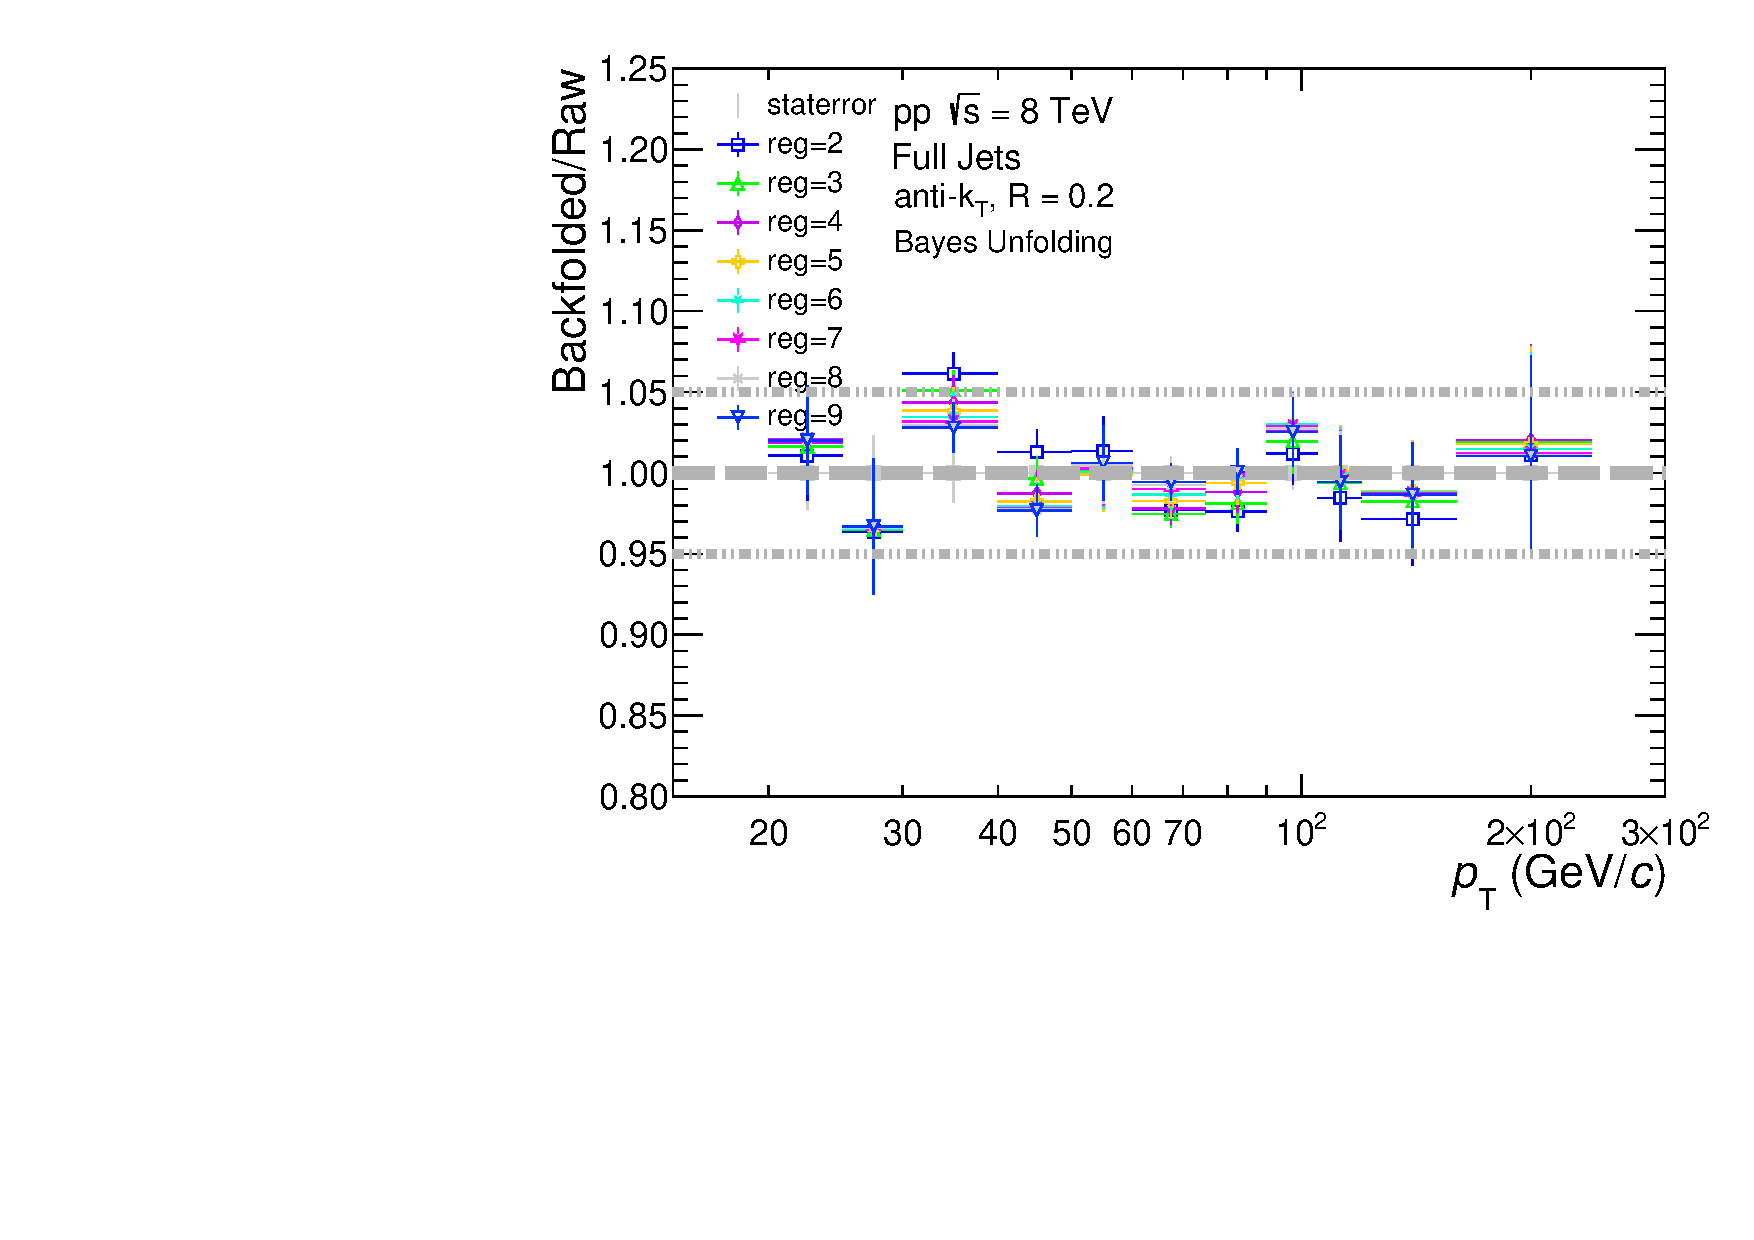
\includegraphics[width=0.49\textwidth]{figures/UnfoldingComparisons/BackfoldedVsRaw/RatioFoldRawBayes_R02.pdf}
        \vfill\null
    \end{multicols}
    \caption{Backfolded spectrum for multiple iterations vs. the raw spectrum for R=0.2 in jets from \pp collisions.}
    \label{fig:BackfoldedRaw}
\end{figure}


Figure~\ref{fig:BackfoldedRaw} shows the comparison of the backfolded spectrum to the uncorrected spectrum for several regularizations for SVD and Bayesian unfolding. This test attempts to re-fold the results by re-applying the response matrix to undo the original process and makes a comparison to the original raw spectrum. The backfolded spectrum should ideally match the raw spectrum as closely as possible.


\begin{figure}[hbt!]
    \centering
    \begin{multicols}{2}
            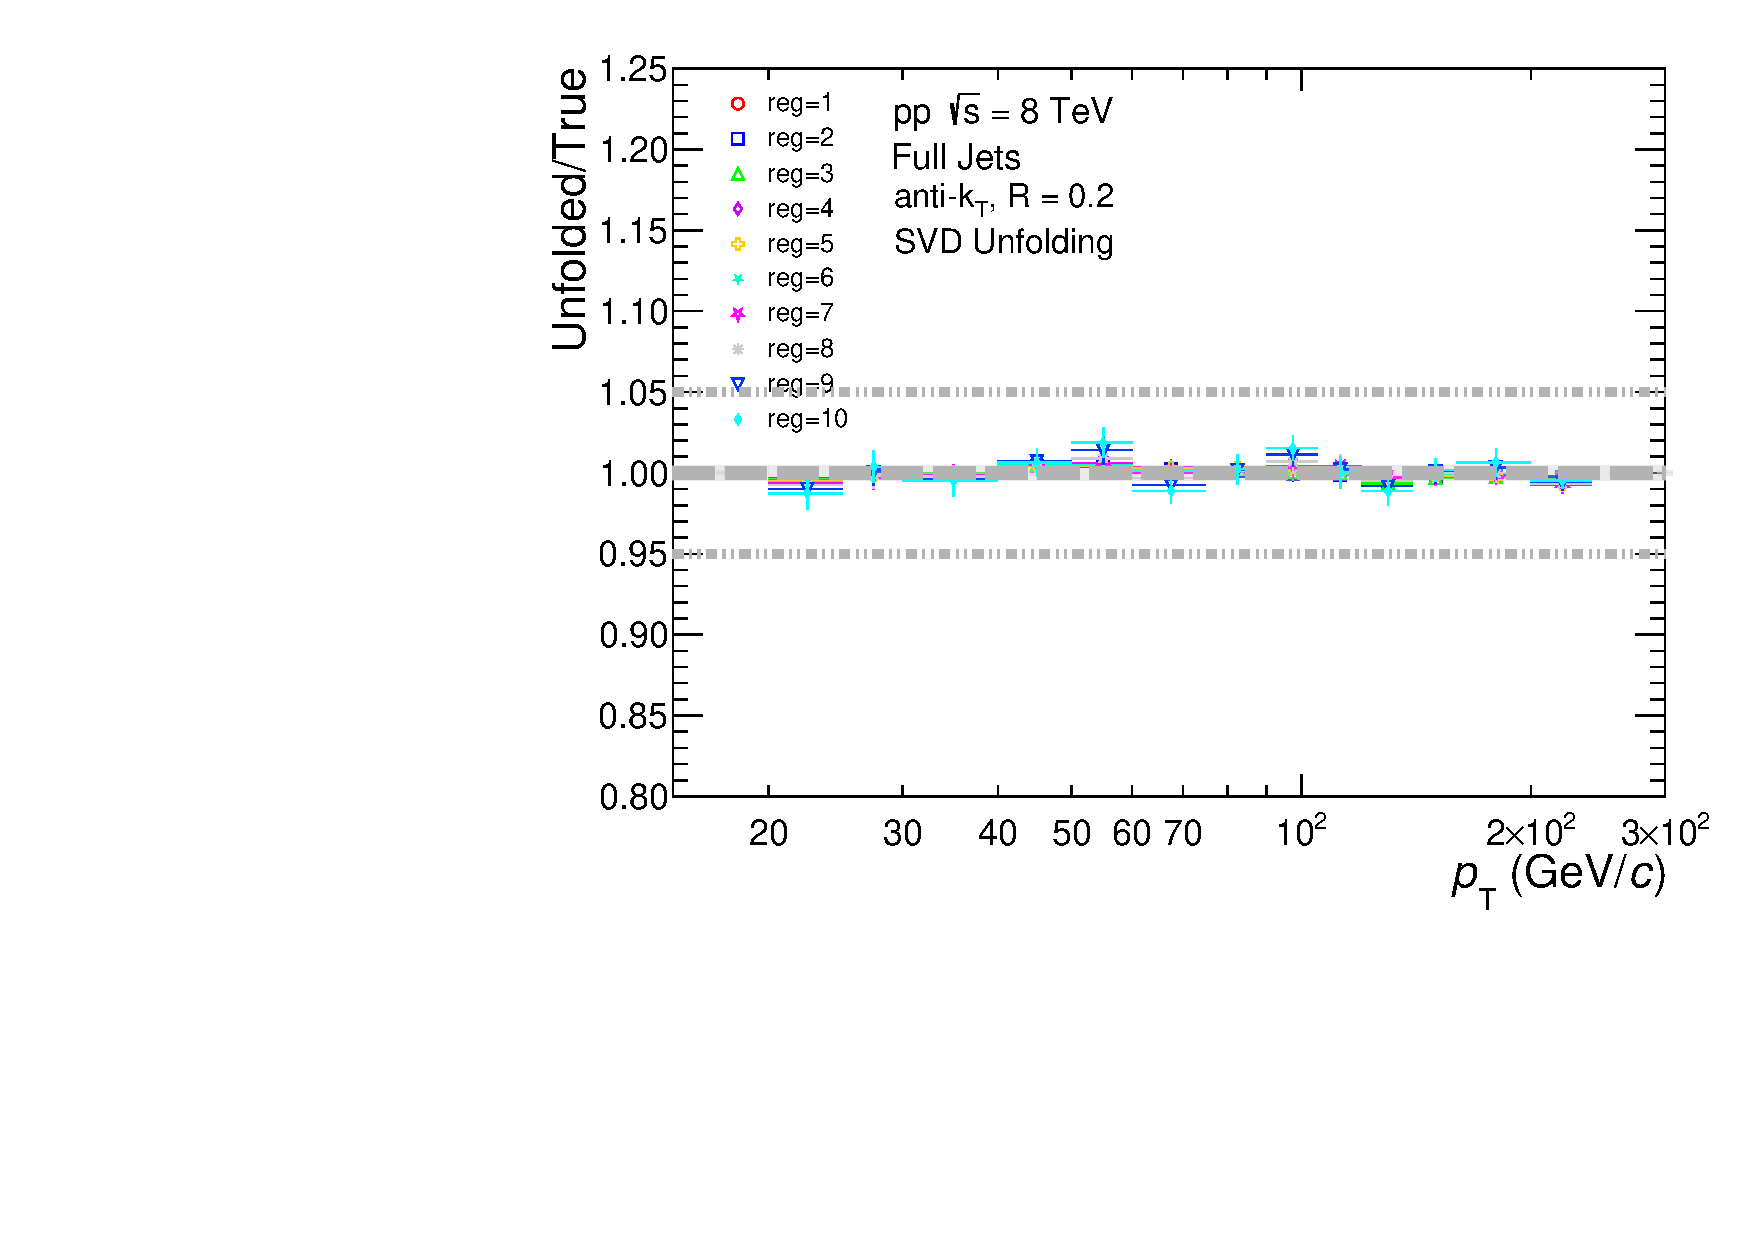
\includegraphics[width=0.49\textwidth]{figures/UnfoldingComparisons/Closure/RatioClosure1DSvd_R02.pdf}
        \vfill\null
        \columnbreak
            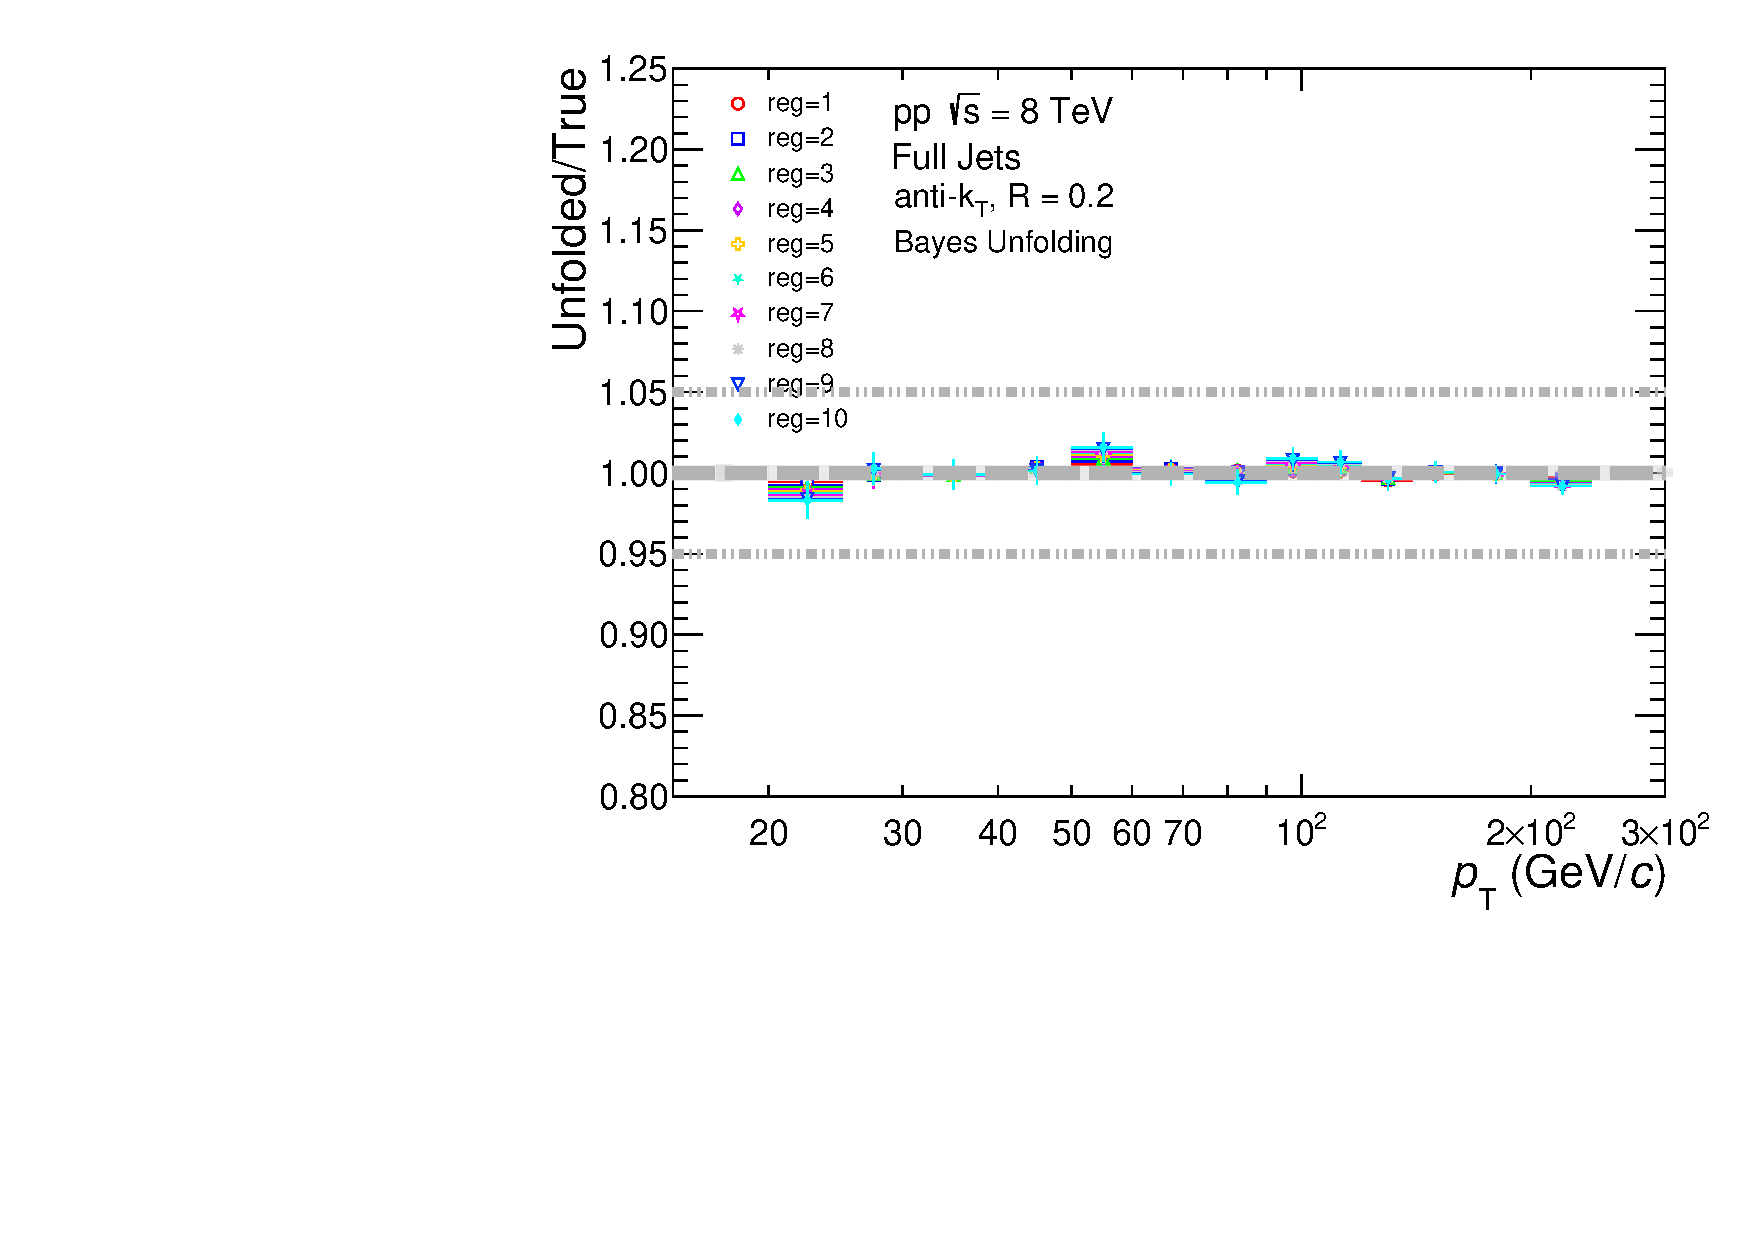
\includegraphics[width=0.49\textwidth]{figures/UnfoldingComparisons/Closure/RatioClosure1DBayes_R02.pdf}
        \vfill\null
    \end{multicols}
    \caption{Closure test for the unfolding of jet resolution parameter R=0.2 in jets from \pp collisions.}
    \label{fig:Closure}
\end{figure}


Figure~\ref{fig:Closure} shows the Monte Carlo closure test for SVD and Bayesian unfolding, where the Monte Carlo sample is split randomly with 20$\%$ used for the smeared spectrum and 80$\%$ used for the response matrix. The test shows agreement between the true spectrum and the unfolded solution.

The same unfolding tests were performed to check the stability of the unfolding process for jets reconstructed in the \pPb dataset. Figure~\ref{fig:RegIterpPb} shows the ratio of the spectra for several regularizations or iterations to the chosen default solution. Convergence is not achieved as quickly as in \pp collisions, but the solution stabilizes with increasing iterations or regularizations. Convergence is not reached as quickly due to low statistics in the trigger transition region causing unfolding instabilities. Figure~\ref{fig:BackfoldedRawpPb} shows the comparison of the backfolded to the raw spectrum. Just as in \pp collisions, the final bins have large uncertainties with central points lying further from unity, but the solution still converges on itself with increasing iterations or regularizations. Figure~\ref{fig:ClosurepPb} shows the Monte Carlo closure tests, which show good convergence at unity within very few iterations or regularizations. Figure~\ref{fig:DVectorpPb} shows the D-vector analysis, which reaches a plateau in a similar range to \pp collisions. All tests show convergence in final \pT range reported. Appendix~\ref{sec:AppendixUnfoldingTestspPb} contains the remaining jet radii.


\begin{figure}[hbt!]
    \centering
    \begin{multicols}{2}
            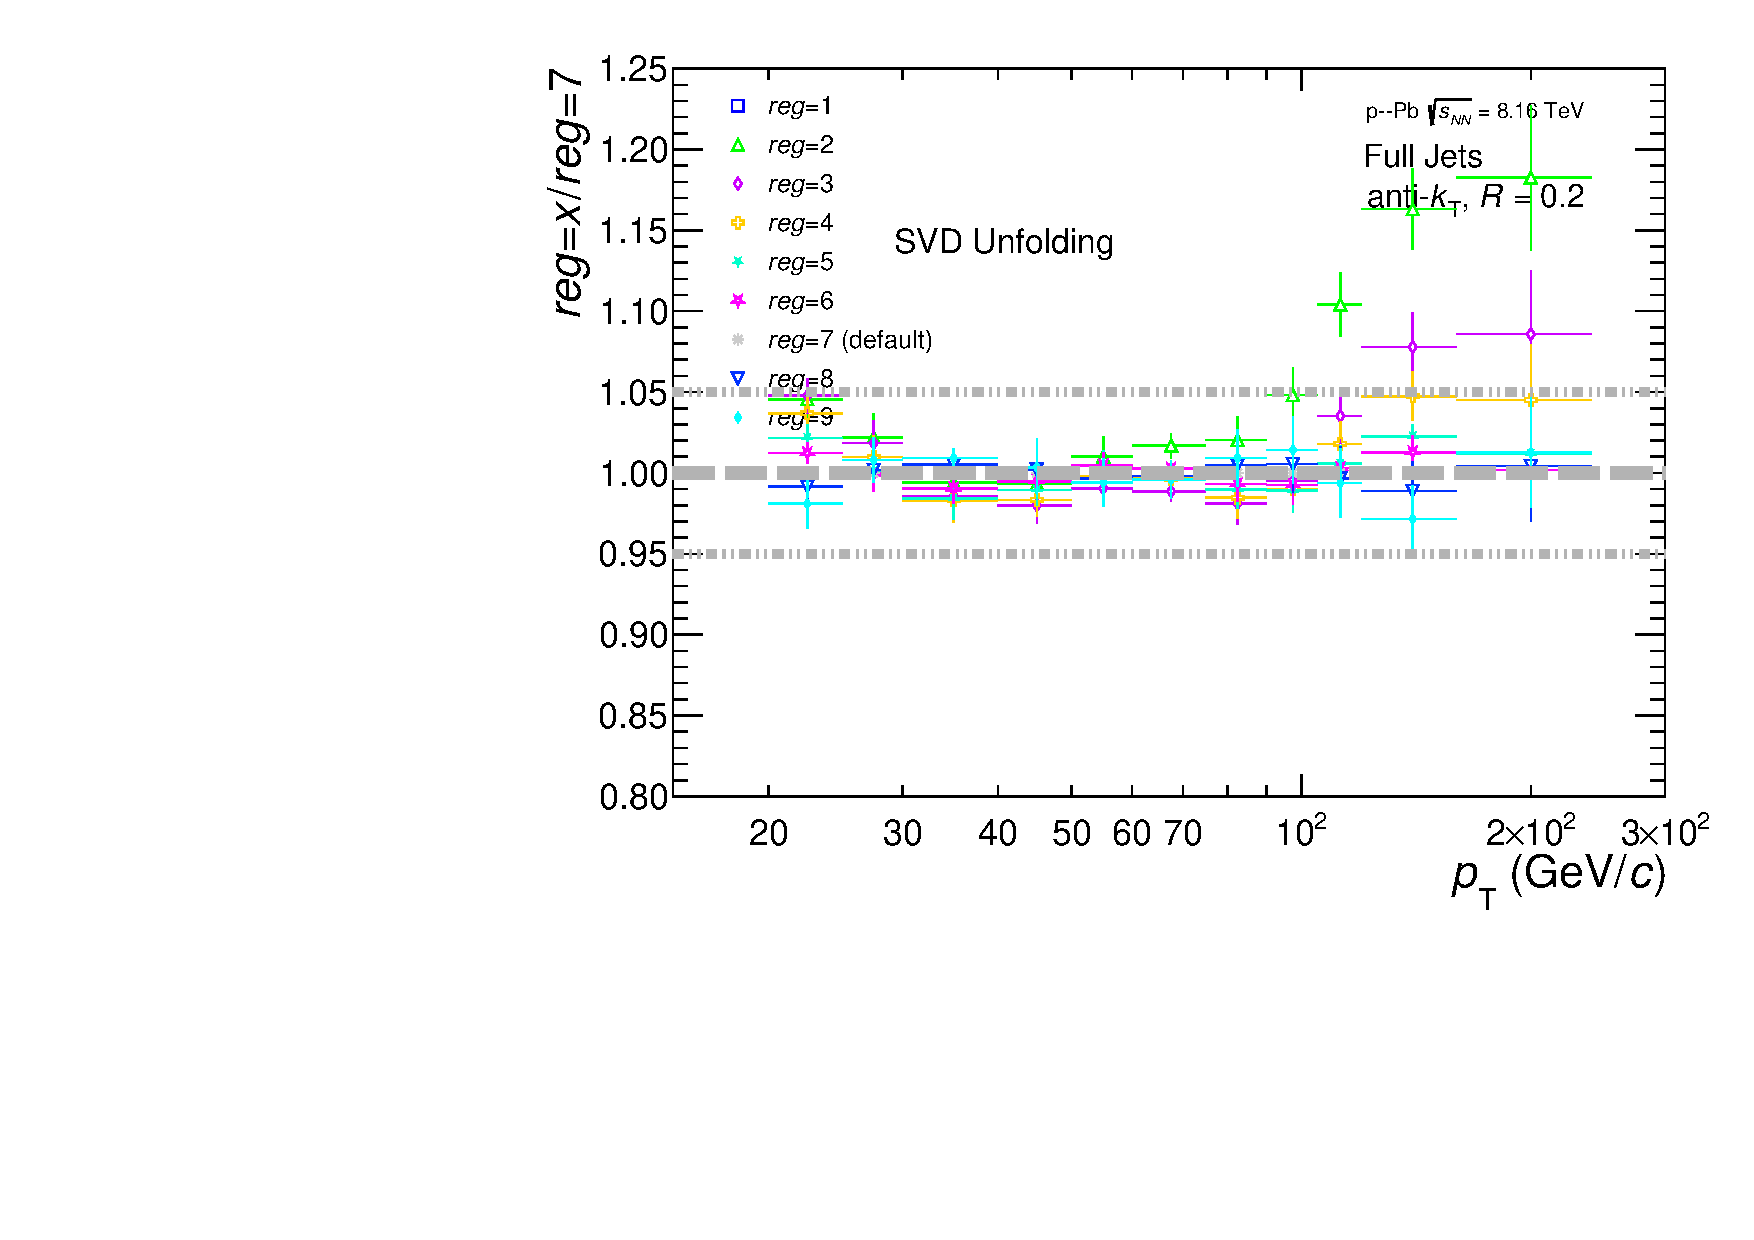
\includegraphics[width=0.49\textwidth]{figures/pPbFigures/UnfoldingComparisons/Regularizations/RatioRegularizationSvd_R02.pdf}
        \vfill\null 
        \columnbreak
            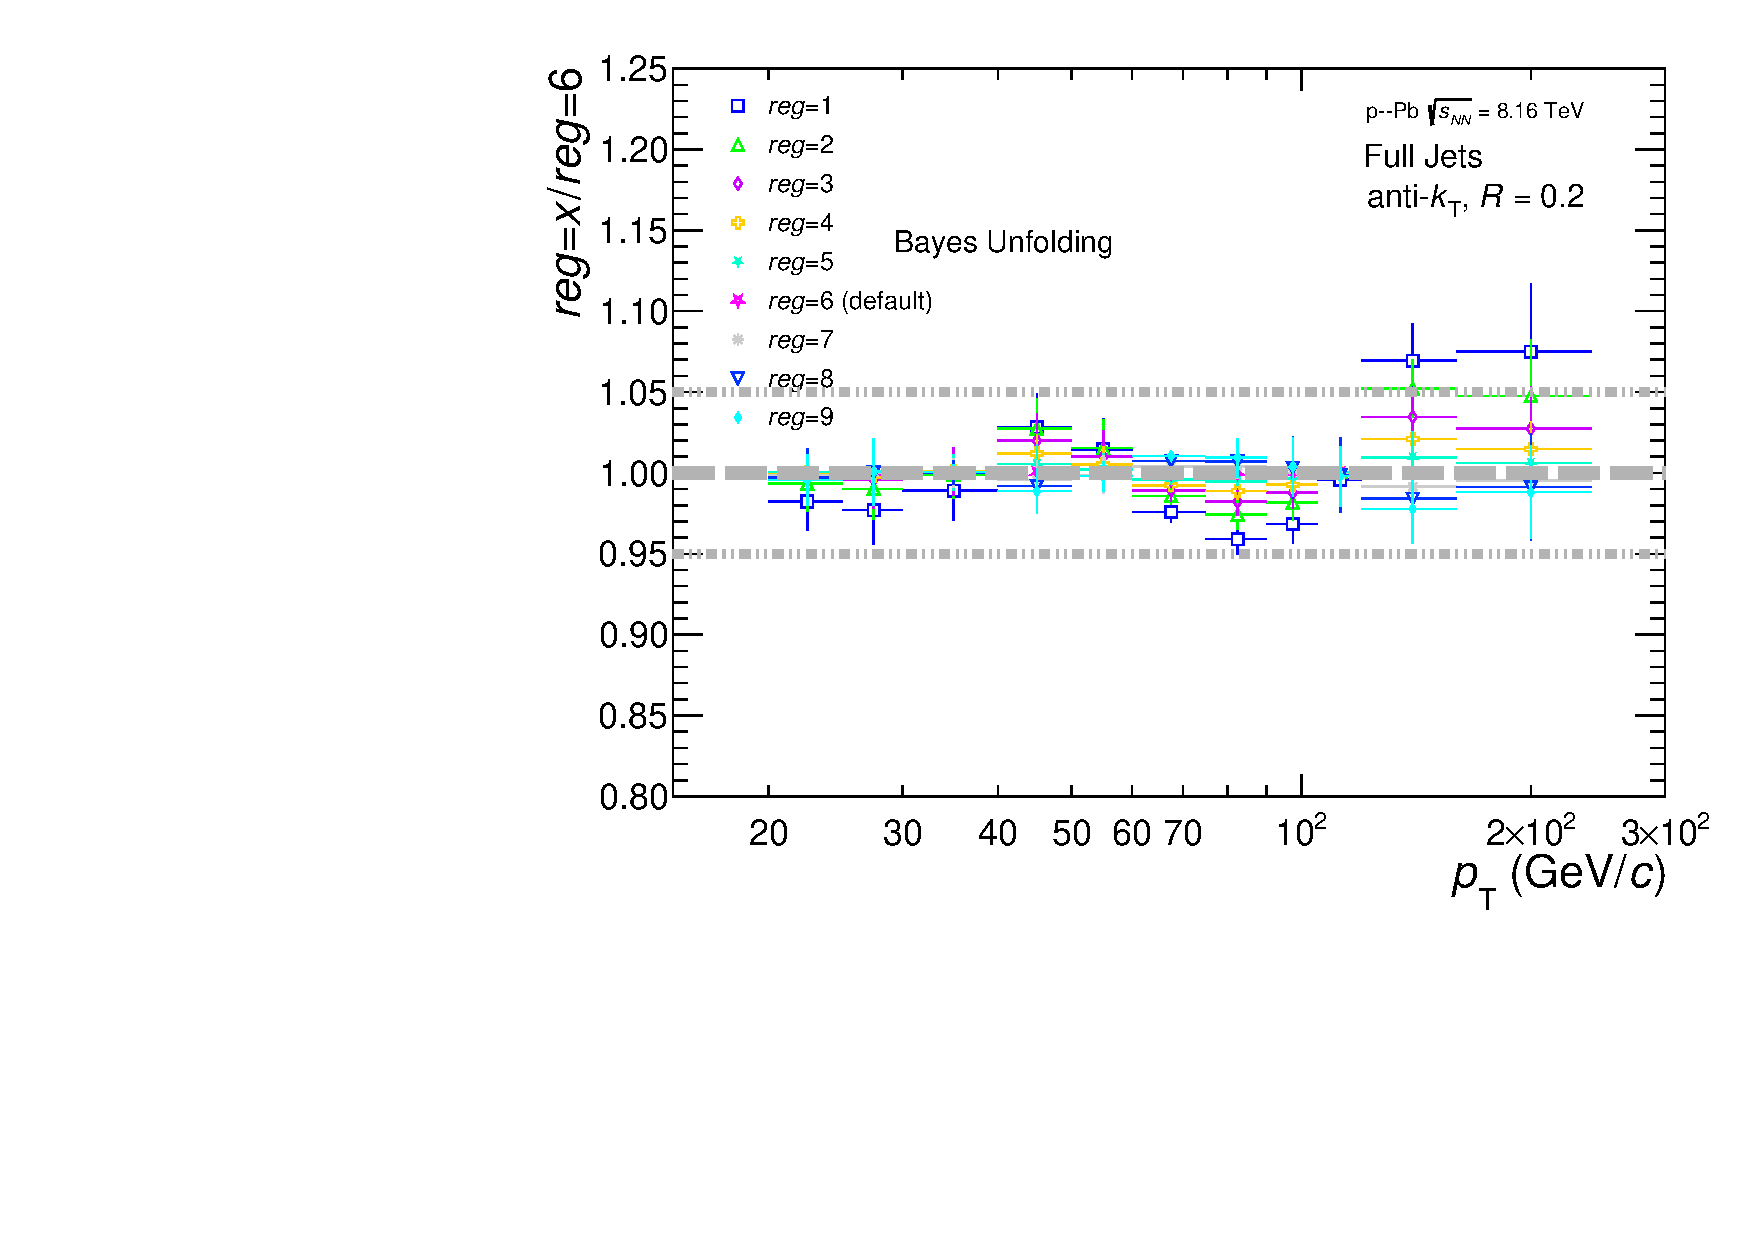
\includegraphics[width=0.49\textwidth]{figures/pPbFigures/UnfoldingComparisons/Regularizations/RatioRegularizationBayes_R02.pdf}
        \vfill\null
    \end{multicols}
    \caption{Regularization dependence for SVD (left) and Bayesian (right) unfolding of jets in \pPb collisions. Iterations are also labeled as "reg" in this plot for visual comparison between the methods.}
    \label{fig:RegIterpPb}
\end{figure}



\begin{figure}[hbt!]
    \centering
    \begin{multicols}{2}
        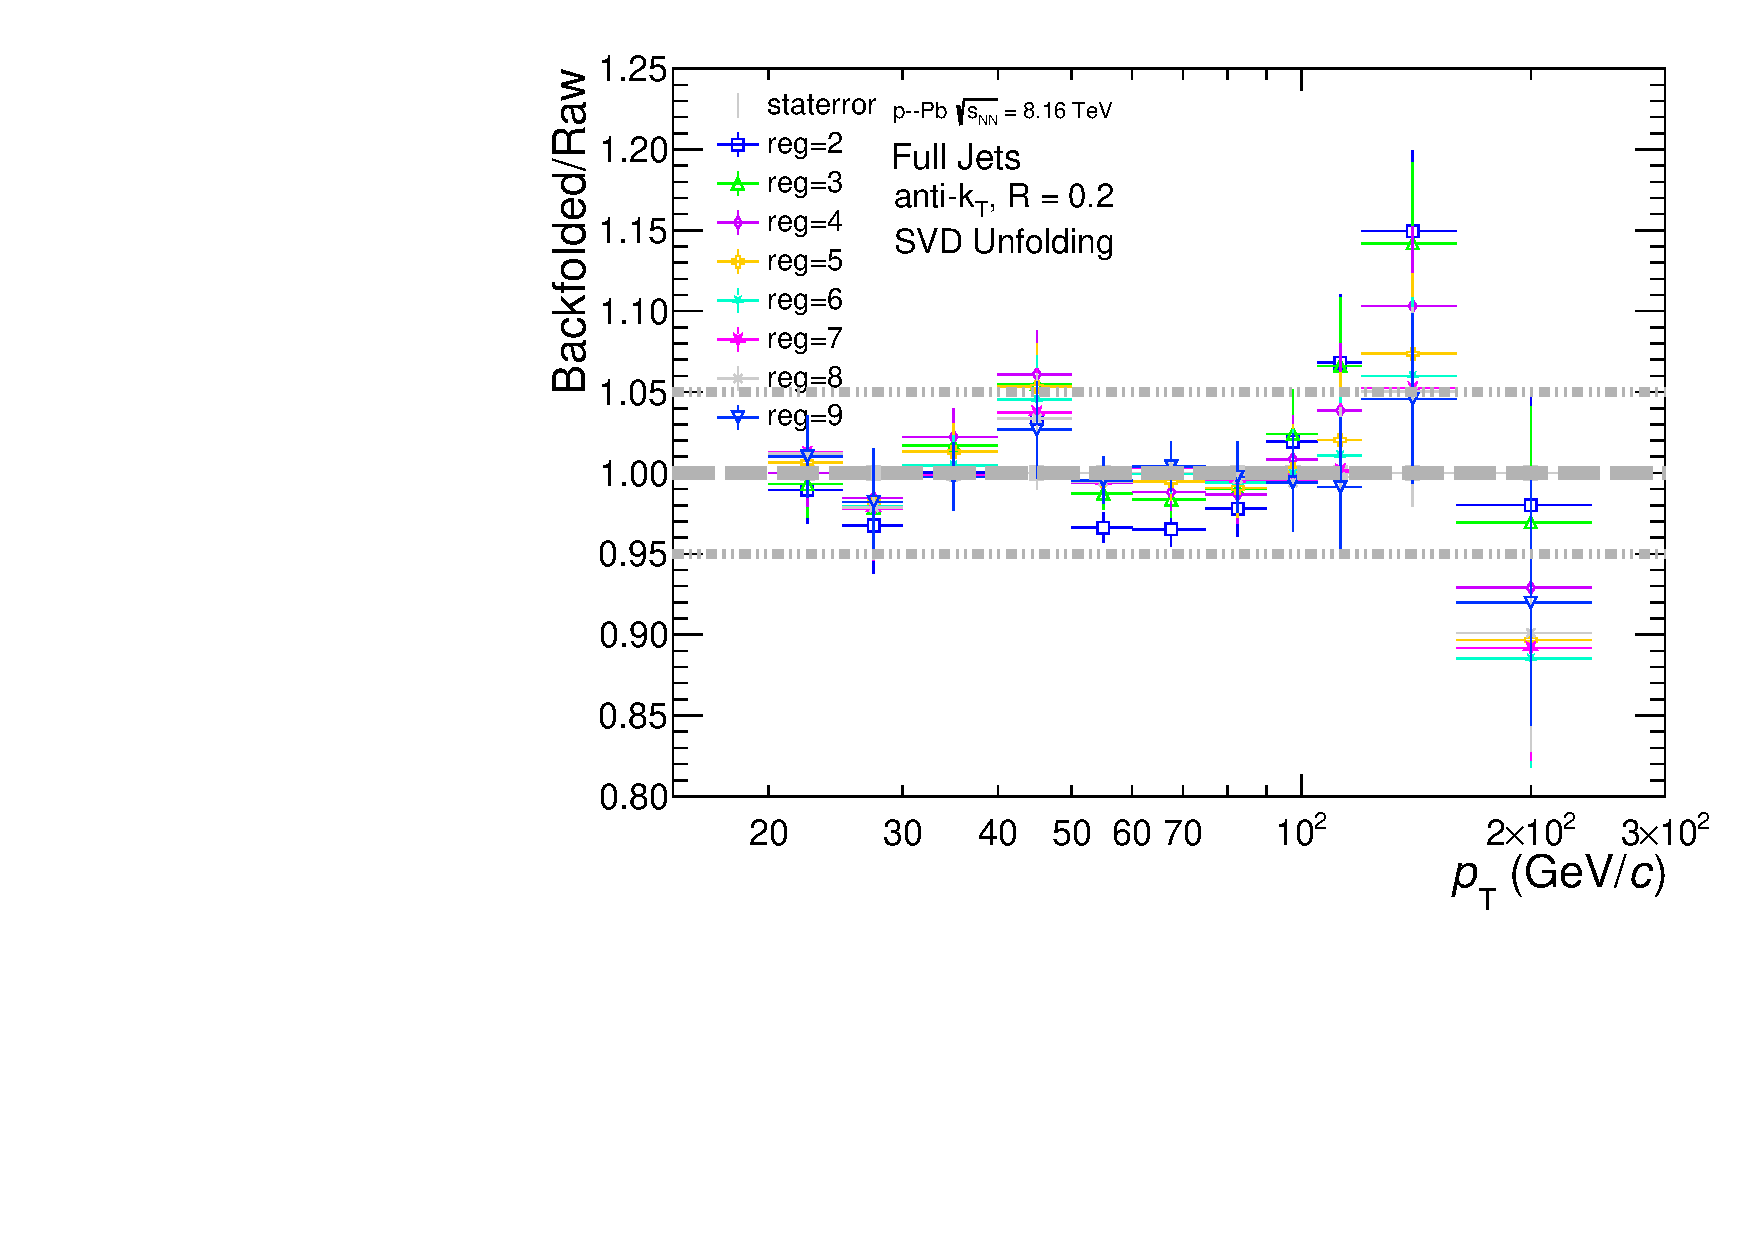
\includegraphics[width=0.49\textwidth]{figures/pPbFigures/UnfoldingComparisons/BackfoldedVsRaw/RatioFoldRawSvd_R02.pdf}
    \vfill\null
    \columnbreak
        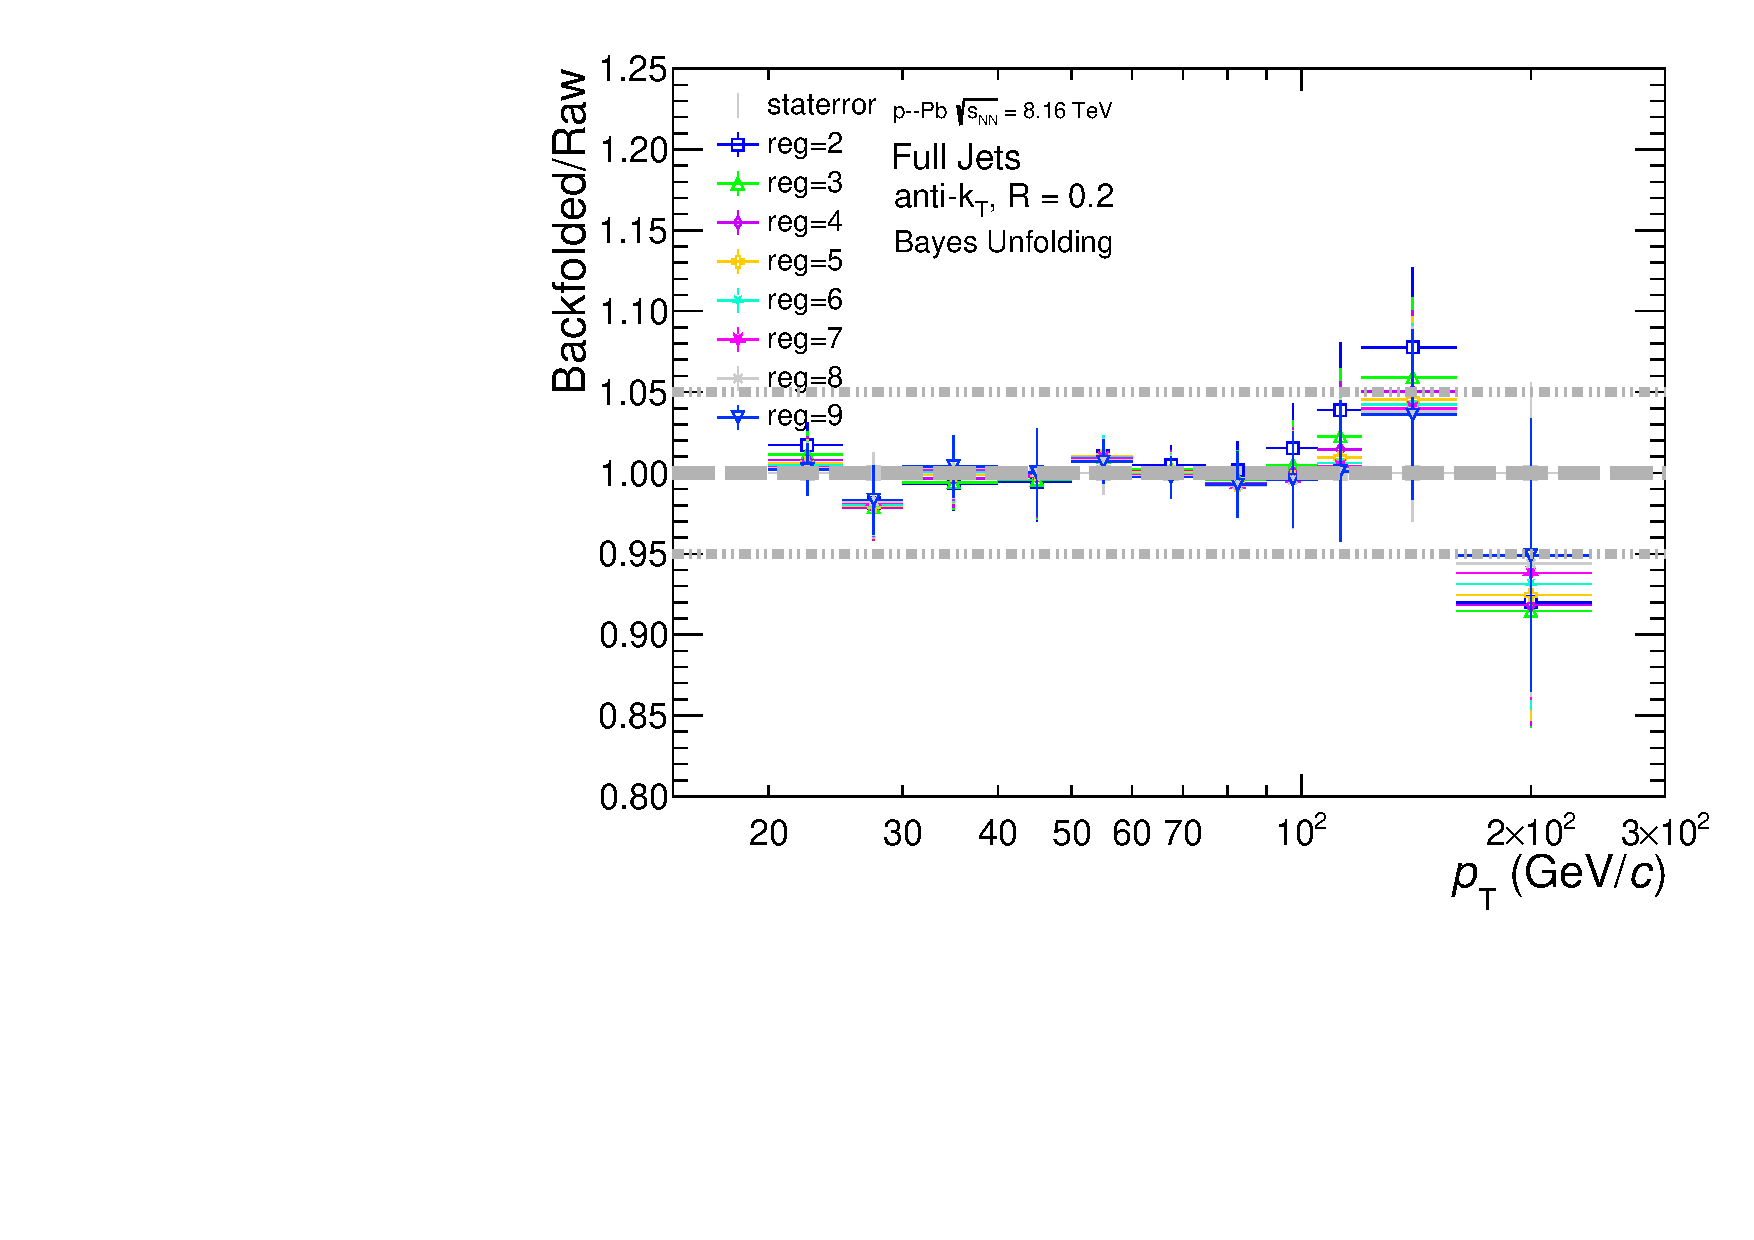
\includegraphics[width=0.49\textwidth]{figures/pPbFigures/UnfoldingComparisons/BackfoldedVsRaw/RatioFoldRawBayes_R02.pdf}
        \vfill\null
    \end{multicols}
    \caption{Backfolded spectrum for multiple iterations vs. the raw spectrum for R=0.2 in jets from \pPb collisions.}
    \label{fig:BackfoldedRawpPb}
\end{figure}



\begin{figure}[hbt!]
    \centering
    \begin{multicols}{2}
            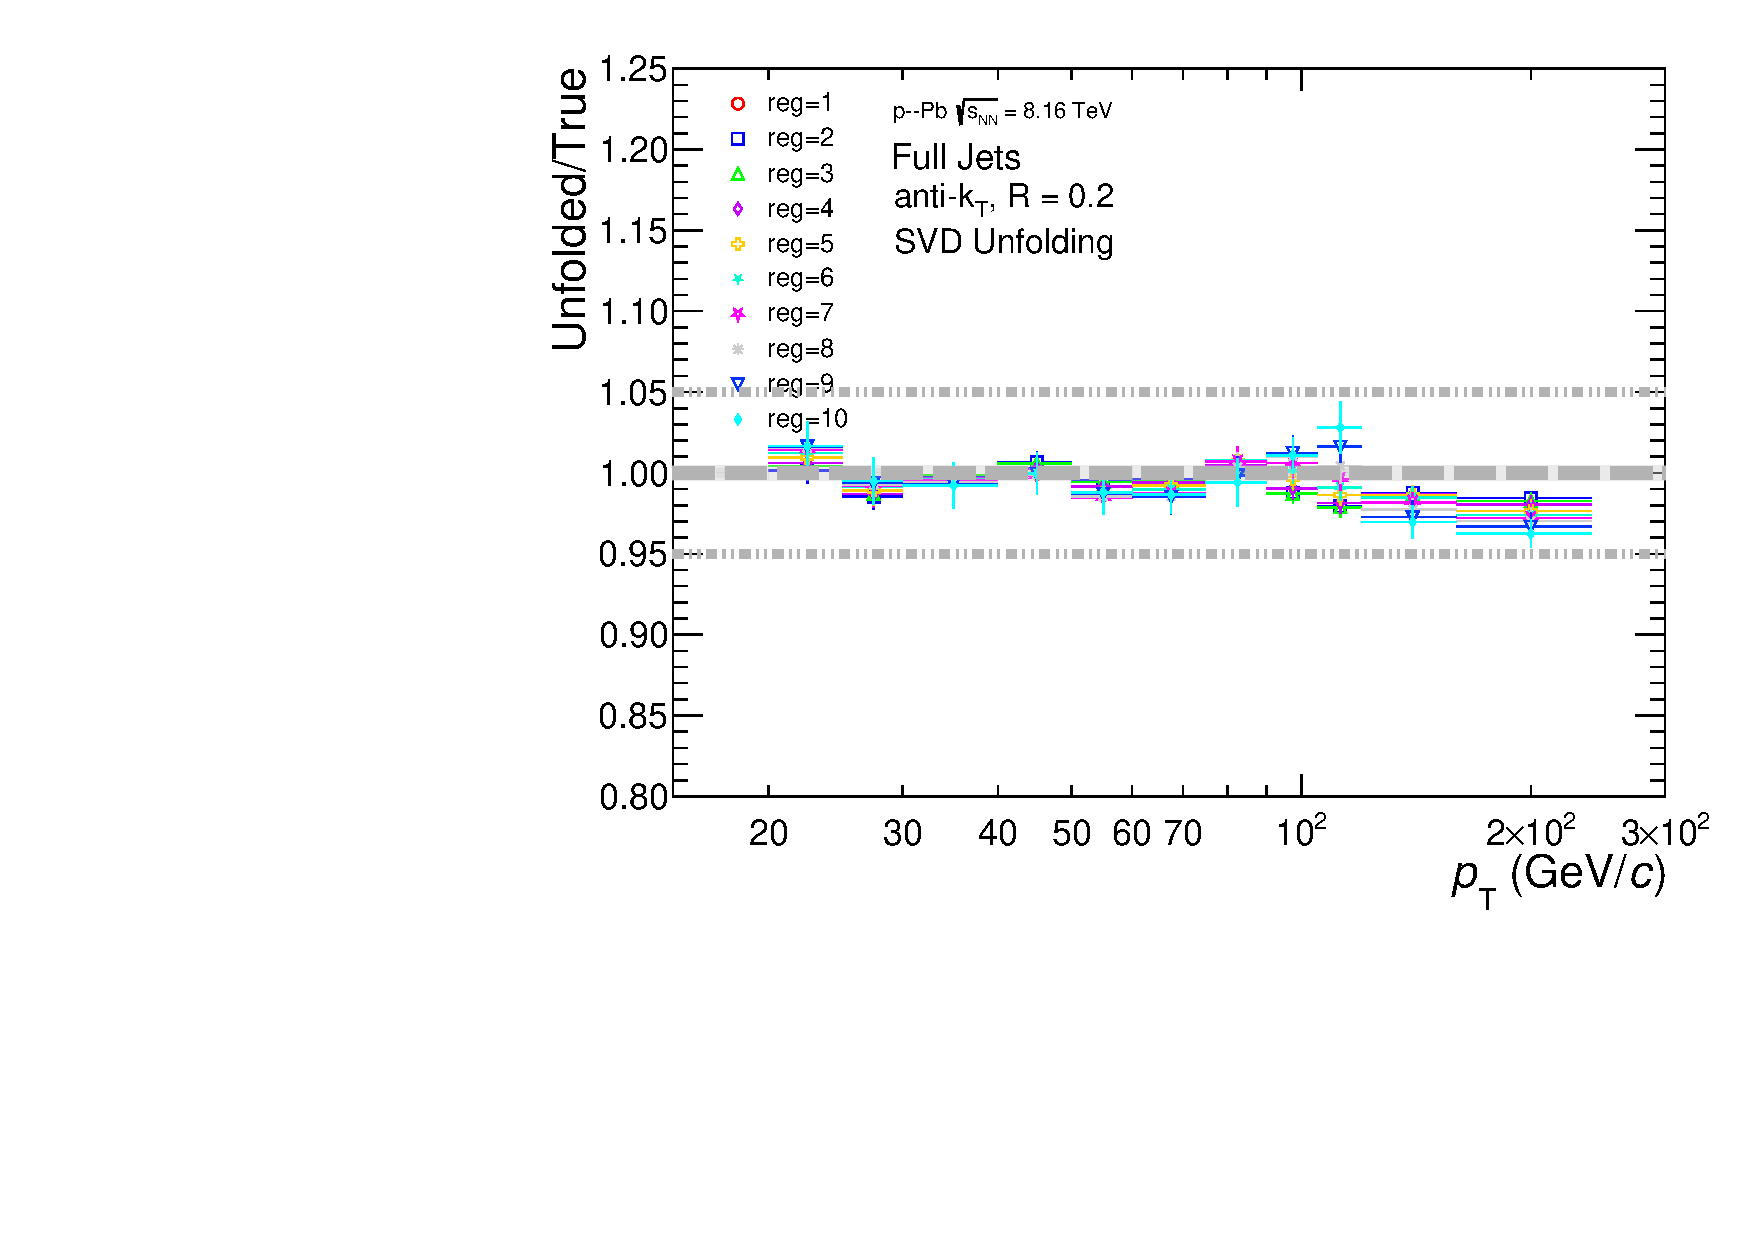
\includegraphics[width=0.49\textwidth]{figures/pPbFigures/UnfoldingComparisons/Closure/RatioClosure1DSvd_R02.pdf}
        \vfill\null
        \columnbreak
            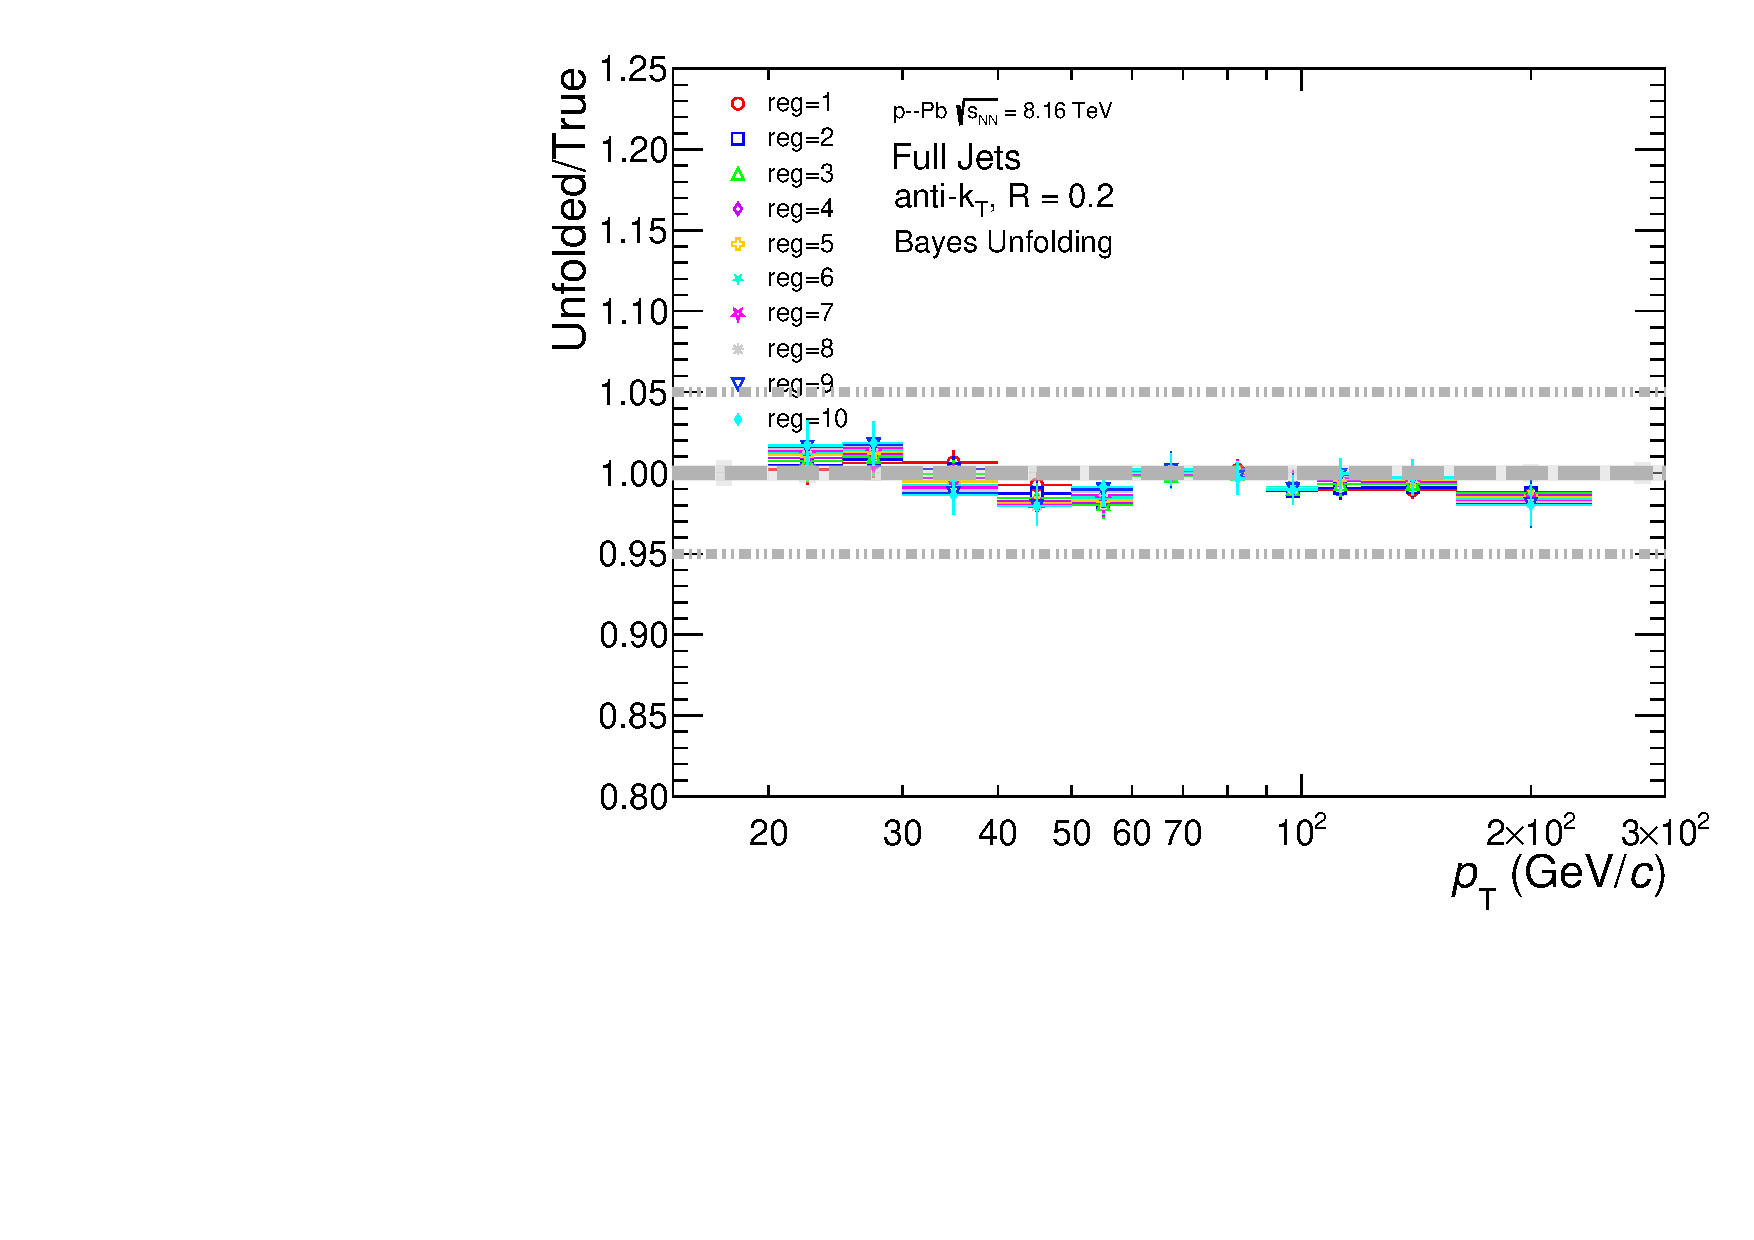
\includegraphics[width=0.49\textwidth]{figures/pPbFigures/UnfoldingComparisons/Closure/RatioClosure1DBayes_R02.pdf}
        \vfill\null
    \end{multicols}
    \caption{Closure test for the unfolding of jet resolution parameter R=0.2 in jets from \pPb collisions.}
    \label{fig:ClosurepPb}
\end{figure}


\begin{figure}[hbt!]
    \centering
    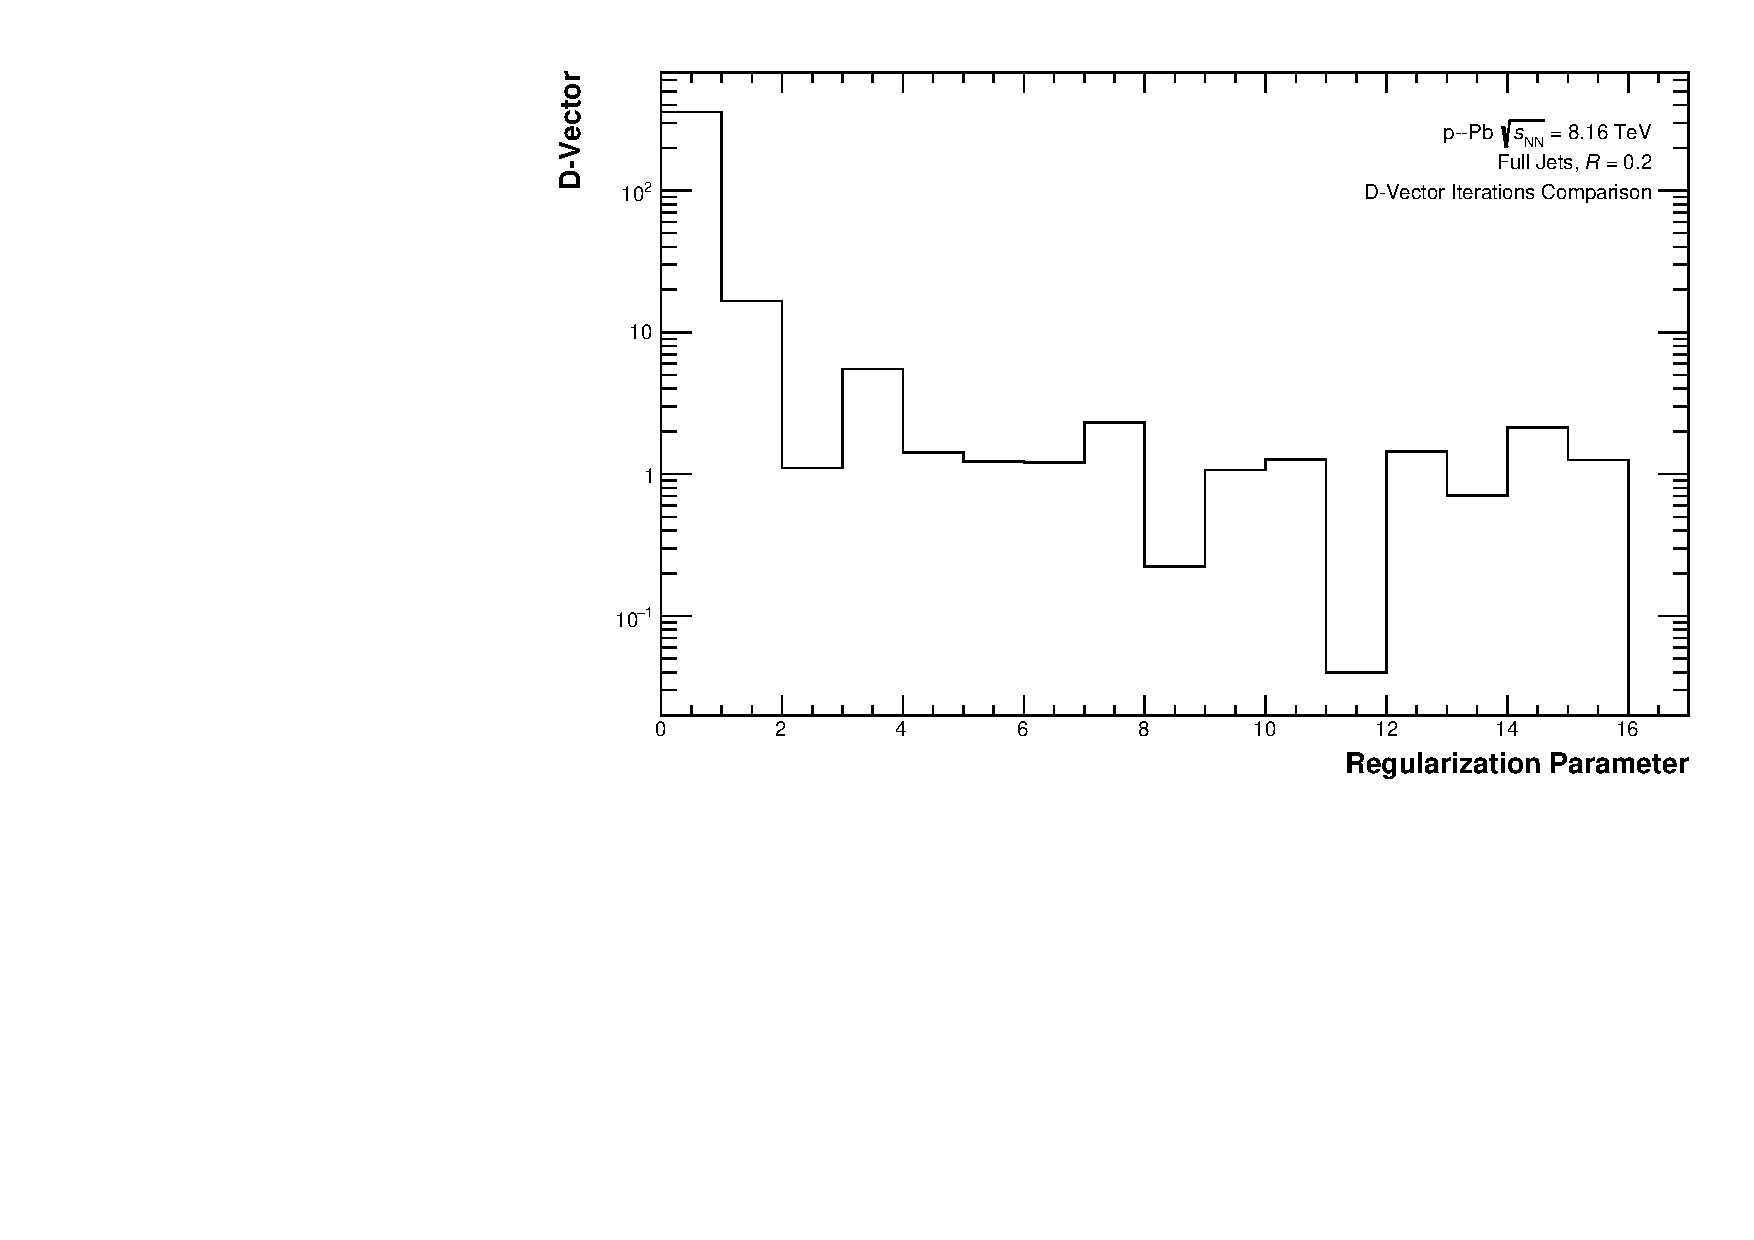
\includegraphics[width=15cm]{figures/pPbFigures/DVector/DVector_R02.pdf}
    \caption{D-Vector comparison for multiple regularizations of SVD unfolding of the jet spectrum for $R$ = 0.2 jets in \pPb collisions.}
    \label{fig:DVectorpPb}
\end{figure}
